%class, papersize a4/letter, size and parksip
\documentclass[letterpaper,11pt,bibliography=totoc,twoside=true,parskip=half]{scrartcl}
%less margins over title
%\usepackage[top=.3cm, bottom=2cm, left=2cm, right=2cm]{geometry}
%Input encoding - chose language
%\usepackage[ngerman]{babel} %alternative for writing German
\usepackage[T1]{fontenc}
\usepackage{lmodern}
\usepackage[utf8]{inputenc}
%
%TODO Set Author, title, and adjust date if neccesary
\newcommand{\AUTOR}{University of California, Irvine}
\newcommand{\TITEL}{CEE224A Transportation Data Analysis I}
\newcommand{\DATUM}{\today} %default date is today
\renewcommand{\DATUM}{Winter Quarter 2019} %change date if neccesary
\author{\AUTOR}
\title{\TITEL}
\date{\DATUM}
%
%settings for PDF
\usepackage[pdftitle={\TITEL},
pdfauthor={\AUTOR}]{hyperref}
%
%setting up headers
%only odd pages in onesides documents
\usepackage[headsepline,automark]{scrlayer-scrpage}
\clearpairofpagestyles
\automark[section]{section}
\automark*[subsection]{}
%\lehead{\pagemark}
%\rohead{\pagemark}
\lohead{\rightmark}
\rehead{\leftmark}
%
%\rofoot{\pagemark}
\ohead{\normalfont \thepage }

%%%%%%%%%%%%%%%%%%%%%%%%%%%%%%%%%%%%%%%%%%
%%Literature
\usepackage[backend=biber,style=apa,url=false,hyperref=false,isbn=false,doi=false,sorting=none]{biblatex}
\addbibresource{lit.bib}
%ignore note field
\AtEveryBibitem{%
	\clearfield{note}%
}
%%%%%%%%%%%%%%%%%%%%%%%%%%%%%%%%%%%%%%%%%%
%Optional Packages for coding, pictures etc.
%\usepackage{listings} %source code environment
%\lstset{
%	language=R,
%	breaklines=true,
%	  numbers=none, %where to put the line-numbers; possible values are (none, left, right)
%	  numbersep=5pt, % how far the line-numbers are from the code
%	  numberstyle=\tiny\color{gray}, % the style that is used for the line-numbers
%	  }
%%
\usepackage{graphicx} %Graphic Packages
\usepackage{tikz,pgf} %Draw Graphic Packages
%
\usepackage{amsmath}	%Mathematic packagees
\usepackage{amsfonts}
\usepackage{amssymb}
%
%Boxes
\usepackage[framemethod=TikZ]{mdframed}
\usepackage{amsthm}
%
%Numbers like 1st etc
\usepackage[super]{nth}
%
%diagobox for tables
\usepackage{diagbox}
%
%licensing
\usepackage{csquotes}
\usepackage[
type={CC},
modifier={by-sa},
version={4.0},
]{doclicense}
%
%set space for roman toc number
\usepackage{tocloft}
\setlength{\cftpartnumwidth}{3.5cm}
%better numbered lists
\usepackage{enumerate}
%%%%%%%%%%%%%%%%%%%%%%%%%%%%%%
%%figure count by section
%\usepackage{chngcntr}
%\counterwithin{figure}{section}
%
%
\newcommand{\myparagraph}[1]{\paragraph{#1}\mbox{}\\}
%figure credits
\newcommand{\credits}[1]{\flushright{\textsf{\tiny #1}}}
%%%%%%%%%%%%%%%%%%%%%%%%%%%%%%
%example renaned
\newcounter{exmp}[section] \setcounter{exmp}{0}
\renewcommand{\theexmp}{\Roman{section}.\arabic{exmp}}
\newenvironment{exmp}[2][]{%
	\refstepcounter{exmp}%
	\ifstrempty{#1}%
	{\mdfsetup{%
			frametitle={%
				\tikz[baseline=(current bounding box.east),outer sep=0pt]
				\node[anchor=east,rectangle,fill=cyan!30]
				{\strut Example~\theexmp};}}
	}%
	{\mdfsetup{%
			frametitle={%
				\tikz[baseline=(current bounding box.east),outer sep=0pt]
				\node[anchor=east,rectangle,fill=cyan!30]
				{\strut Example~\theexmp:~#1};}}%
	}%
	\mdfsetup{innertopmargin=10pt,linecolor=cyan!30,backgroundcolor=cyan!5,%
		linewidth=2pt,topline=true,%
		frametitleaboveskip=\dimexpr-\ht\strutbox\relax
	}
	\begin{mdframed}[]\relax%
		\label{#2}}{\end{mdframed}}
%%%%%%%%%%%%%%%%%%%%%%%%%%%%%%
\newcounter{defi}[section]\setcounter{defi}{0}
\renewcommand{\thedefi}{\Roman{section}.\arabic{defi}}
\newenvironment{defi}[2][]{%
	\refstepcounter{defi}%
	\ifstrempty{#1}%
	{\mdfsetup{%
			frametitle={%
				\tikz[baseline=(current bounding box.east),outer sep=0pt]
				\node[anchor=east,rectangle,fill=violet!30]
				{\strut Definition~\thedefi};}}
	}%
	{\mdfsetup{%
			frametitle={%
				\tikz[baseline=(current bounding box.east),outer sep=0pt]
				\node[anchor=east,rectangle,fill=violet!30]
				{\strut Definition~\thedefi:~#1};}}%
	}%
	\mdfsetup{innertopmargin=10pt,linecolor=violet!30,backgroundcolor=violet!5,%
		linewidth=2pt,topline=true,%
		frametitleaboveskip=\dimexpr-\ht\strutbox\relax
	}
	\begin{mdframed}[]\relax%
		\label{#2}}{\end{mdframed}}
%figures
\newcounter{fig}[section]\setcounter{fig}{0}
\renewcommand{\thefig}{\Roman{section}.\arabic{fig}}
\newenvironment{fig}[3][]{%
	\begin{figure}[#3]
	\refstepcounter{fig}%
	\ifstrempty{#1}%
	{\mdfsetup{%
			frametitle={%
				\tikz[baseline=(current bounding box.east),outer sep=0pt]
				\node[anchor=east,rectangle,fill=lime!20]
				{\strut Figure~\thefig};}}
	}%
	{\mdfsetup{%
			frametitle={%
				\tikz[baseline=(current bounding box.east),outer sep=0pt]
				\node[anchor=east,rectangle,fill=lime!20]
				{\strut Figure~\thefig:~#1};}}%
	}%
	\mdfsetup{innertopmargin=10pt,linecolor=lime!20,%
		linewidth=2pt,topline=true,%
		frametitleaboveskip=\dimexpr-\ht\strutbox\relax
	}
	\begin{mdframed}[]\relax%
		\label{#2}}{\end{mdframed}\end{figure}
	}
%%%%%%%%%%%%%%%%%%%%%%%%%%%%%%%%%%%%%%%%
%famous statisticans
\newcounter{famo}\setcounter{famo}{0}
\renewcommand{\thefamo}{\roman{famo}}
\newenvironment{famo}[2][]{%
	\refstepcounter{famo}%
	\ifstrempty{#1}%
	{\mdfsetup{%
			frametitle={%
				\tikz[baseline=(current bounding box.east),outer sep=0pt]
				\node[anchor=east,rectangle,fill=olive!30]
				{\strut Famous Statisticians~\thefamo};}}
	}%
	{\mdfsetup{%
			frametitle={%
				\tikz[baseline=(current bounding box.east),outer sep=0pt]
				\node[anchor=east,rectangle,fill=olive!30]
				{\strut Famous Statisticians~\thefamo:~#1};}}%
	}%
	\mdfsetup{innertopmargin=10pt,linecolor=olive!30,backgroundcolor=olive!5,%
		linewidth=2pt,topline=true,%
		frametitleaboveskip=\dimexpr-\ht\strutbox\relax
	}
		\newpage\begin{mdframed}[]\relax%
		\label{#2}}{\end{mdframed}} % check pagebreaks
%%%%%%%%%%%%%%%%%%%%%%%%%%%%%
%Page Margins
\usepackage[%top=.3cm, bottom=2cm, left=2.2cm, right=2.2cm
]{geometry}
%
%Heading number schemata
\makeatletter% wegen @ in den \p@ (siehe De-TeX-FAQ)
\renewcommand*{\thesection}{\Roman{section}}
\renewcommand*{\thesubsection}{\Roman{section}.\arabic{subsection}}
%\renewcommand*{\p@subsection}{\thesection~}
\renewcommand*{\thesubsubsection}{\Roman{section}.\arabic{subsection}.\Alph{subsubsection}}
%\renewcommand*{\p@subsubsection}{\p@subsection\thesubsection~}
\makeatother% wegen \makeatletter (siehe De-TeX-FAQ)
%Change title font
\addtokomafont{disposition}{\rmfamily}
%Appendix
\usepackage[titletoc]{appendix}
%emph as bold
%\renewcommand{\emph}[1]{\color{Brown}{\textbf{#1}}}
%%%%%%%%%%%%%%%%%%%%%%%%%%%%%%%%%%%%%%%%%%%
%%Symbol list
%\usepackage[intoc]{nomencl}
%%\renewcommand{\nomname}{List of Symbols and Abbreviations}
%\newcommand*{\nom}[2]{#2 (#1)\nomenclature[A]{#1}{#2}}
%\newcommand*{\sym}[2]{#2 (#1)\nomenclature[S]{#1}{#2}}
%%\renewcommand\nomenclature[3][X]{\nomenclature[#1#3]{#2}{#3}}
%\renewcommand{\nomgroup}[1]{%
%	\ifstrequal{#1}{A}{\item[\sffamily{\textbf{Acronyms}}]}{%
%		\ifstrequal{#1}{S}{\vspace{20pt} \item[\sffamily{\textbf{Symbols}}]}{}}}%
%%%%%%%%%%%%%%%%%%%%%%%%%%%%%%%%%%%%%%%%%%%%
\begin{document}
\maketitle
\tableofcontents
\addsec{Preface}
This scriptum is based on the notes taken in the lecture \emph{CEE224A Transportation Data Analysis I} by Professor Jean-Daniel Saphores, held at the Institute of Transportation Studies at University of California in Irvine in the winter quarter 2019. This course is designed as an introduction to statistical and econometric tools for analyzing datasets for applications in the field of transportation science. It is a graduate level course with basic knowledge of probability and statistics as prerequisites. The lecture is on based on the literature recommended. The notes have been extended with further information, references and explanatory figures. Even though this notes have been gleaned with utmost care by  \href{mailto:jfrische@uci.edu}{Jens Frische}, it is highly unlikely that there are no mistakes in this script. If you are aware of one or want to extend the scope further, you can find all necessary \LaTeX\space source files here: \href{https://github.com/soaringhigh/NotesUciCee224}{\texttt{https://github.com/soaringhigh/NotesUciCee224}}\nocite{Washington.2011}\nocite{Angrist.2009}\nocite{Stock.2015}\nocite{Kennedy.2008}\nocite{Wooldridge.2016}\nocite{Train.2009}\nocite{Conover.1999}

\doclicenseThis

\printbibliography[title={Recommended Literature}]\
\addsec{Recommended Journals}
		Journal of Transport and Land Use.\\
		Transportation Research Part A-F.\\
		Transportation.\\
		Transport Review.
%TODO: better pictures for bias etc instead of self-drawn, pictures in famous statistican potraits
\section{Descriptive Statistics}
%%%%%%%%%%%%%%%%%%%%%%%%%%%%%
	Descriptive statistics give us tools to summarize and interpret data.
	\begin{defi}[Statistics]{defi:stat}
		Analyzing characteristics of a sample to interpret characteristics of the population. 
	\end{defi}
	\begin{defi}[Probability Theory]{defi:prob}
		Knowing characteristics of a population to find the probability for a sample.
	\end{defi}		
	Why is it important to know your sample? Because knowing the variability in the dataset allows to find abnormalities. Such abnormalities can either be invalid data records which need to be filtered out, or remarkable observations pointing towards unexpected subpopulations, which deserve to learn more about them.
\subsection{Point Estimates}
	\subsubsection{Central tendency}
		\begin{defi}[Arithmetic Mean]{defi:mean}
			Consider a sample $x_1,x_2,...,x_n$ with the size $n$ from a population of the size $N$.
			\begin{align*}
				\text{Sample mean: }\;\bar{X}&=\frac{\sum\limits_{i=1}^{n}x_i}{n}\\
				\text{Population mean: }\;\mu&=\frac{\sum\limits_{i=1}^{N}x_i}{N}		
			\end{align*}			
		\end{defi}
		The \emph{arithmetic mean} is very common because it is easy to calculate, but sensitive to extreme values which can easily influence the value in their direction. A remedy to this problem is the usage of the \emph{median}.
		\begin{defi}[Median]{defi:median}
		In an ordered sample ($x_1\leq x_2 \leq ... x_n$), the median is $x_{int \frac{1}{2}}$ such that half of the observations are larger and the other half are smaller values. It is identical with the \nth{50}-percentile.
		\end{defi}
		Another useful measure is the \emph{mode}. If the distribution of a sample data is symmetric and unimodal (thus, has one mode), then there is a unique mode which is equal to the mean and equal to the median.
		\begin{defi}[Mode]{defi:mode}
			The mode is the value that occurs the most frequently.
		\end{defi}
	\subsubsection{Central relative standing}
		Consider an ordered sample $x_1\leq x_2 \leq ... x_n$. We can characterize the concept of the median to calculate percentiles. For example, the \nth{10}-percentile is such that 10\% of the observations are smaller and and 90\% are larger. The goal is to get information about the distribution of the data.
	\subsubsection{Measures of variability}
		Measures of variability quantify the dispersion of the data (typically around the mean).
		\begin{defi}[Range]{defi:range}
			The range is the difference between the highest and lowest value.
			\begin{equation*}
				x_{max}-x_{min}
			\end{equation*}
		\end{defi}
		\begin{defi}[Interquartile Range]{defi:iqrange}
			The interquartile range is the difference between the \nth{3} and the \nth{1} quartile.
			\begin{equation*}
			x_{75}-x_{25}
			\end{equation*}
		\end{defi}
		\begin{defi}[Variance]{defi:variance}
			The variance is the average sum of the squares of deviations to the mean.
			\begin{align*}
				\text{Sample variance: }\;s^2&=\frac{\sum\limits_{i=1}^{n}(x_i-\bar{X})^2}{n-1}\\
				\text{Population variance: }\;\sigma^2&=\frac{\sum\limits_{i=1}^{N}(x_i-\mu)^2}{N}
			\end{align*}
		\end{defi}
		Empirical experience has shown that dividing by $n-1$ gives better results for the variance with small sample sizes. The expressions $\bar{X}$ and $s^2$ are \emph{estimators} for the population mean $\mu$ and variance $\sigma^2$.
		\begin{defi}[Estimator]{defi:estimator}
			An estimator is a rule which tells how to combine and conclude
			sample data to obtain estimate a population characteristic.
		\end{defi}
		\begin{defi}[Standard Deviation]{defi:standarddev}
			The standard deviation is the square root of the variance.
			\begin{align*}
			\text{Sample standard deviation: }\;s&=\sqrt{s^2}\\
			\text{Population standard deviation: }\;\sigma&=\sqrt{\sigma^2}
			\end{align*}
		\end{defi}
		\begin{defi}[Empirical Rule]{defi:emprule}
			The empirical or 68–95–99.7 rule states the approximated percentage of values that lie within a certain range of the mean for data that is normal distributed.
			\begin{align*}
				\Pr(\mu-1\sigma \le X \le \mu+1\sigma) &\approx 0.6827 =68\% \\
				\Pr(\mu-2\sigma \le X \le \mu+2\sigma) &\approx 0.9545 =95\%\\
				\Pr(\mu-3\sigma \le X \le \mu+3\sigma) &\approx 0.9973 =99.7\%
			\end{align*}
		\end{defi}	
		\begin{defi}[z-score]{defi:z}
			A sample $x_1,x_2,...,x_n$ has the normalizing z-scores $z_1,z_2,...,z_n$.
			\begin{equation*}
				z_i=\frac{x_i-\bar{X}}{s}
			\end{equation*}
		\end{defi}
		\begin{exmp}[Expected Value of Random Variables]{exmp:expected}
			Consider a  sample $x_1,x_2,...,x_n$ as a random variable coming from $x\Rightarrow E(x) =\mu ,\, var(x) =\sigma^2$.\\
			Then $z$ is also a random variable: $z\equiv\frac{x-\mu}{\sigma}$.
			\begin{align*}
				E(z)&=E(\frac{x-\mu}{\sigma})=\frac{1}{\sigma}\left(E(x)-\mu\right)=0\\
				var(z)&=var(\frac{x-\mu}{\sigma})-\frac{1}{\sigma}var(x-\mu).
			\end{align*}
			For the random variable $y$: $var(y)=E\left((y-E(y)^2)\right)$.
			\begin{align*}
				var(y+\alpha)&=E\left((y+\alpha)-E(y+\alpha))^2\right)\\
				&=E\left((y-E(y))^2\right)\\
				&=var(y)
			\end{align*}			
		\end{exmp}
		\begin{defi}[Chebyshev's Theorem]{defi:chebyshev}
			For any sample, the proportion of observations whose z-score has an absolute value $z\leq k\,\epsilon\,\mathbb{N}^+$ is no less (so greater or equal) than $1-\frac{1}{k^2}$.
		\end{defi}
		\begin{align*}
			k=1\;\longrightarrow\; 1-\frac{1}{k^2}=1-\frac{1}{1^2}=0\;&\longrightarrow\;\text{no statement. Empirical rule: }68\%\\
			k=2\;\longrightarrow\; 1-\frac{1}{k^2}=1-\frac{1}{2^2}=\frac{3}{4}\;&\longrightarrow\;\geq 75\%\text{. Empirical rule: }95\%\\
			k=3\;\longrightarrow\; 1-\frac{1}{k^2}=1-\frac{1}{3^2}=\frac{8}{9}\;&\longrightarrow\;\geq 88.9\%\text{. Empirical rule: }99.7\%\\
		\end{align*}
		Named after the Russian mathematician Pafnuty Chebyshev, the theorem allows to make a statement about how much values are within an certain range. This information is less specific than that coming from the empirical rule, but Chebyshev's theorem is applicable to \emph{any} sample, regardless of its distribution whereas the 68–95–99.7 rule strictly requires normal distributed data.
	\subsubsection{Measures of the shape of a distribution}
		\begin{defi}[Skewness]{defi:skewness}
			The skewness is a measure for the degree of asymmetry of a distribution.
			\begin{align*}
				\text{Population skewness: }\;\gamma_1&={E}\left[\left(\frac{X-\mu}{\sigma}\right)^3 \right]= \frac{\mu_3}{\sigma^3}= \frac{E\left[(X-\mu)^3\right]}{( E\left[ (X-\mu)^2 \right] )^{3/2}}\\
				\text{Sample skewness estimator: }\; g_1&={E}=\frac{\frac{1}{n}\sum\limits_{i=1}^n (x_i-\bar{X})^3}{\left(\frac{1}{n}\sum\limits_{i=1}^n (x_i-\bar{X})^2\right)^\frac{3}{2}}
			\end{align*}			
			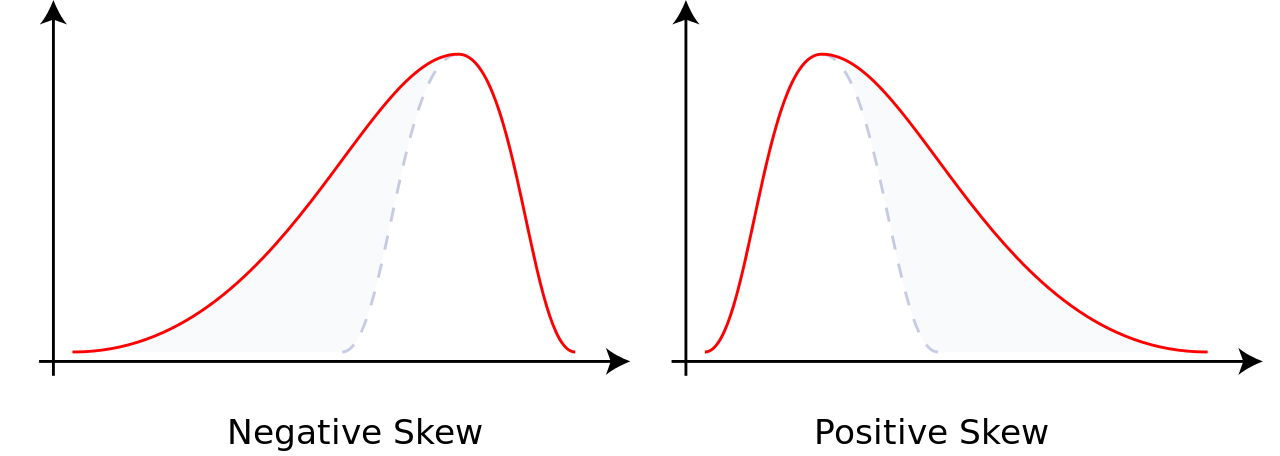
\includegraphics[width=\textwidth]{P01skew.png}	
			\credits{By Rodolfo Hermans (Godot) at Wikipedia Commons. CC BY-SA 3.0.}									
		\end{defi}
		For small sample sizes (but at least $x\geq 3$), the MATLAB-method delivers better estimates.
		\begin{equation*}
			G_1=\frac{\sqrt{n(n-1)}}{n-2}g_1
		\end{equation*}
		The skewness is the \nth{3} normalized moment when the distribution is seen as an area. The variance as shown in definition \ref{defi:variance} then is the \nth{2} central moment, whereas the mean shown in definition \ref{defi:mean} is the \nth{1} moment, i.e. the center of gravity.
		\begin{defi}[Kurtosis]{defi:kurt}
		The kurtosis (from the Greek word for \emph{curved}) is a measure about how heavy the tails of a distribution are compared to the center around the mean.
			\begin{align*}
			\text{Population kurtosis: }\;\kappa&=E\left(\left(\frac{x-\mu}{\sigma}\right)^4\right)\\
			\text{Sample kurtosis: }\; k_1&=\frac{\frac{1}{n}\sum\limits_{i=1}^n (x_i-\bar{x})^4}{\left(\frac{1}{n}\sum\limits_{i=1}^n (x_i-\bar{x})^2\right)^2}\\
			\text{Sample kurtosis estimator with bias correction: }\\
			k_0=\frac{n-1}{(n-2)(n-3)}\left((n-1)k_1-3(n-1)\right)&+3\\
			\text{The estimator requires: }\; n\geq 4,\qquad\lim\limits_{n\rightarrow\infty}\frac{(n-1)(n+1)}{(n-2)(n-3)}&=3
			\end{align*}					
			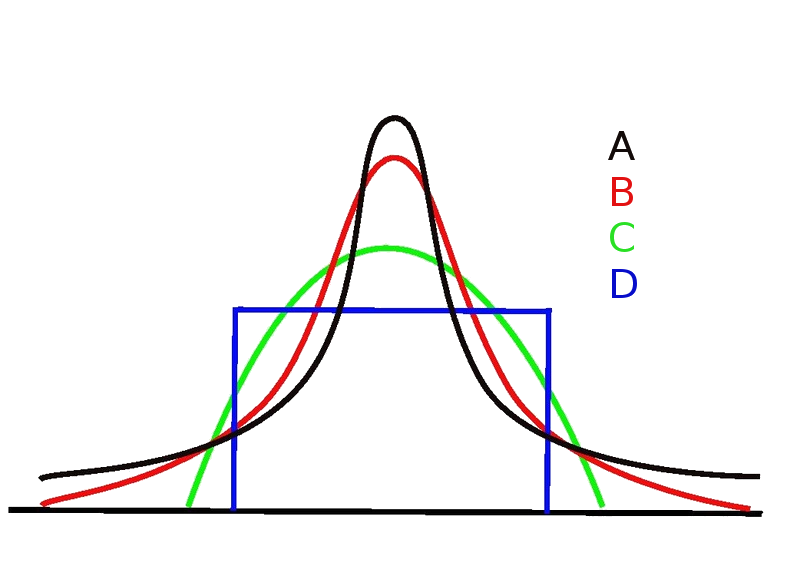
\includegraphics[width=\textwidth]{P00kurtosis.png}
			The graphic shows a normal distribution with different kurtosis, graph A has the highest.
			\credits{By Joxemai at Wikipedia Commons. CC BY-SA 3.0.}												
		\end{defi}
		The kurtosis gives us information on how prone to outliers a distribution is. Following the scheme of the skewness (\ref{defi:skewness}) as the \nth{3} moment, the kurtosis is the \nth{4} moment of a distribution. A normal distribution has  the kurtosis $\kappa=3$.
	\subsubsection{Measures of association}
		Often, we are interested in more than one variable in a time. The \emph{covariance} tells how two variables are related when one changes. The measure is not normalized and has an unit, so mostly informative is the sign. With a positive covariance, an increase in one value corresponds with a greater value for the other one, the covariance is positive. If the values change in different directions, the covariance is negative.
		\begin{defi}[Covariance]{defi:cov}
			Consider two random variables $x, y$.
			\begin{align*}
			\text{Sample covariance: }\;cov(x,y)_s&=\frac{\sum\limits_{i=1}^n(x_i-\bar{X})(y_i-\bar{y})}{n-1}\\
			\text{Population covariance: }\;cov(x,y)_p&=\frac{\sum\limits_{i=1}^N(x_i-\mu_x)(y_i-\mu_y)}{N}\\
			\mu_x&=E(x),\;\mu_y=E(y)
			\end{align*}					
		\end{defi}
		To address the problem that the covariance only indicated the direction in which to variables are related, it can be normalized to state the degree of linear association. This measure is called the \emph{correlation}.
		\begin{defi}[Correlation]{defi:cor}
			Consider two random variables $x, y$ with the covariance $cov(x,y)$. 
			\begin{align*}
			\text{Sample correlation: }\;r&=\frac{cov_{s}(x,y)}{s_x s_y}\\
			\text{Population correlation: }\;\rho&=\frac{cov_{p}(x,y)}{\sigma_x \sigma_y}\\
			|r|&\leq 1,\;|\rho|\leq 1
			\end{align*}
		\end{defi}		
		\begin{exmp}[Showing that the correlation is not greater than 1]{exmp:rho}
			Let $a_i=x_i-\bar{X}$ and $b_i=y_i-\bar{y}$. Let $f(z)=\sum (a_i z + b_i)^2 \geq 0$. Expand:
			\begin{align*}
				f(z)=z^2(a_1^2+a_2^2+\cdots+a_N^2)+z(2a_1 b_1+2a_2 b_2+\cdots+2a_N b_N)+(b_1^2+b_2^2+\cdots+b_N^2).
			\end{align*}
			Consider $f(z)=0$. There is no solution unless $a_i z + b_i = 0 \;\forall\; i, z$.		
			\begin{gather*}
				\alpha x^2+\beta x + \gamma = 0\\ \Delta=\beta^2-4\alpha\gamma\\
				\text{Cases }\;\begin{cases}
					\Delta>0, \qquad x^*=\frac{-\beta \pm \sqrt{\Delta}}{2\alpha}\\
					\Delta=0, \qquad x^*=\frac{-\beta}{2\alpha},\;\text{two equal square root solutions}\\
					\Delta>0, \qquad \text{no real solution}
				\end{cases}
			\end{gather*}	
			In this case,
			\begin{equation*}
				\Delta=4\left(\sum a_i b_i\right)^2-4\left(\sum a_i^2 \sum b_i^2\right)\leq 0.
			\end{equation*}
			This is necessarily since $f(z)\geq0$. Hence,
			\begin{align*}
				\left(\frac{\sum\limits_{i=1}^N(x_i-\mu_x)(y_i-\mu_y)}{N}\right)^2&\leq\frac{\sum\limits_{i=1}^N(x_i-\mu_x)^2}{N}\,\frac{\sum\limits_{i=1}^N(y_i-\mu_y)^2}{N}\\
				\left|\frac{\sum\limits_{i=1}^N(x_i-\mu_x)(y_i-\mu_y)}{N}\right|&\leq\sigma_x \sigma_y\\
				\left|\frac{\sum\limits_{i=1}^N(x_i-\mu_x)(y_i-\mu_y)}{N\sigma_x \sigma_y}\right|&\leq 1\\
				\Longrightarrow |\rho|&\leq 1
			\end{align*}
		\end{exmp}
\begin{famo}[John Graunt]{famo:graunt}
	\emph{John Graunt} (April 24, 1620 – April 18, 1674) was \emph{one of the first demographers}, though by profession he was a haberdasher (i.e., he sold small articles for sewing, such as buttons, ribbons, zips).
	
	He was born in London, the eldest of seven or eight children of Henry and Mary Graunt. His father was a draper who had moved to London from Hampshire. In February 1641, John Graunt married Mary Scott, with whom he had one son and three daughters.
	
	He worked in his father's shop until his father died in 1662, and became influential in the City. He served in various ward offices, becoming a common councilman about 1669–71, warden of the Drapers' Company in 1671 and a major in the trained band.
	
	His house was destroyed in the Great Fire of London and he encountered other financial problems leading eventually to bankruptcy. His daughter became a nun in a Belgian convent and Graunt decided to convert to Catholicism at a time when Catholics and Protestants were struggling for control of England and Europe, leading to prosecutions for recusancy. He died of jaundice and liver disease at the age of 53.
	
	With William Petty, \emph{he developed early human statistical and census methods that later provided a framework for modern demography}. He is credited with producing the first life table, giving probabilities of survival to each age. In addition, he is considered one of the first experts in epidemiology, since his famous book was concerned mostly with public health statistics.
	
	His book \enquote{Natural and Political Observations Made upon the Bills of Mortality} (1663) used analysis of the mortality rolls in early modern London as Charles II and other officials attempted to create a system to warn of the onset and spread of bubonic plague in the city. Though his system was not fully created, Graunt's work resulted in the first statistically based estimation of the population of London.
	
	He presented his work to the Royal Society and was subsequently elected a fellow in 1662 with the endorsement of the King. 
	\credits{Source: \url{https://en.wikipedia.org/wiki/John_Graunt}}
\end{famo}\pagebreak
\subsection{Methods for Displaying Data}
	Visualizing the data is useful for
	\begin{itemize}
		\item detecting influential observations,
		\item identifying outliers, and
		\item inspecting data and understanding its distributions. 
	\end{itemize}
	\subsubsection{Histograms}
		Histograms as in figure \ref{fig:hist} are used to display the frequency or density of different values. The values are classified in \emph{bins} representing a range of values the variable of interest can take.			
		\begin{fig}[Histogram]{fig:hist}{!htb}
			\centering
			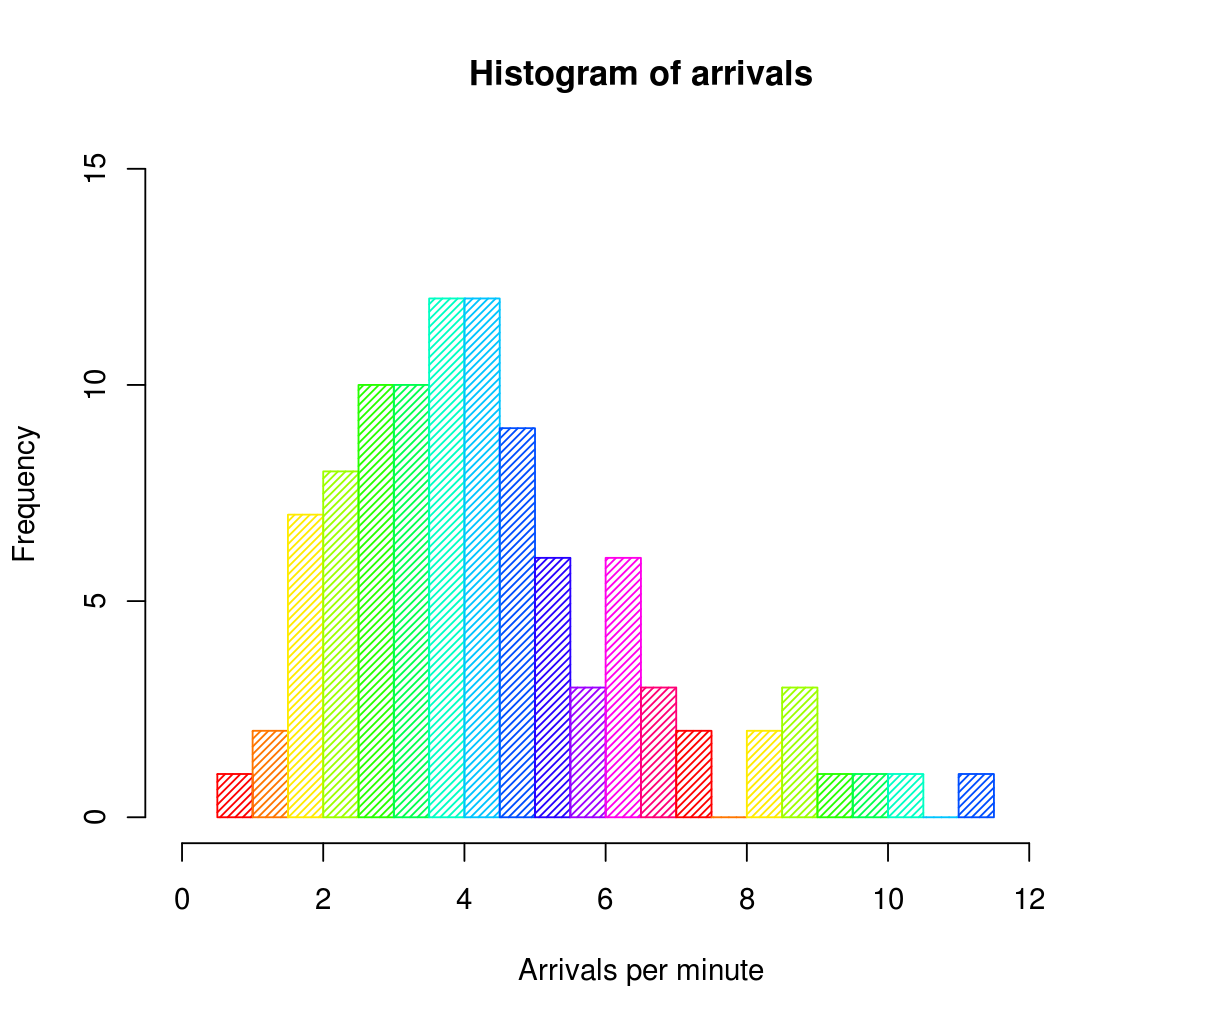
\includegraphics[width=0.95\textwidth,trim={0 1cm 0 5cm},clip]{P02hist.png}
			\credits{By Daniel Penfield at Wikipedia Commons. CC BY-SA 3.0.}
		\end{fig}
\begin{famo}[John Tukey]{famo:tukey}
		\emph{John Wilder Tukey} (June 16, 1915 – July 26, 2000) was an American mathematician.	Born in New Bedford, Massachusetts, he earned a B.A. in 1936 and M.Sc. in 1937, in chemistry, from Brown University, before moving to Princeton University where he received a Ph.D. in mathematics. 
	
	During World War II, he worked at the Fire Control Research Office and collaborated with Samuel Wilks and William Cochran. After the war, he returned to Princeton, where he divided his time between the university and AT\&T Bell Laboratories. \emph{He became a full professor at 35 and was founding chairman of the Princeton statistics department in 1965}. 
	
	He was awarded the \emph{National Medal of Science by President Nixon in 1973}, and the IEEE Medal of Honor in 1982 \enquote{For his contributions to the spectral analysis of random processes and the fast Fourier transform (FFT) algorithm}.

	He is known for developing the FFT algorithm, the box plot, the Tukey range test, the Tukey $\lambda$ distribution, the Tukey test of additivity, and the Teichmüller–Tukey lemma. 
	
	He also made many contributions and articulated the important distinction between exploratory data analysis and confirmatory data analysis. In particular, he believed that much statistical methodology placed too great an emphasis on the latter. A. D. Gordon offered the following summary of Tukey's principles for statistics: 
	\begin{itemize}
		\setlength{\itemsep}{0pt}
		\setlength{\parskip}{0pt} 		
		\item The usefulness and limitation of mathematical statistics, 
		\item \emph{the importance of having methods of statistical analysis that are robust to violations of the assumptions underlying their use},  
		\item the need to amass experience of the behavior of specific methods of analysis in order to provide guidance on their use,  
		\item the importance of \emph{allowing the possibility of data's influencing the choice of method by which they are analyzed}, 
		\item the need for statisticians to reject the role of 'guardian of proven truth', and to resist attempts to provide once-for-all solutions and tidy overunifications, 
		\item the iterative nature of data analysis, and 
		\item the importance of the increasing power, availability and cheapness of computers,
		\item with John von Neumann, he introduced the word \enquote{bit} short for \enquote{binary digit}. 
		\item Tukey's 1958 paper \enquote{The Teaching of Concrete Mathematics} contained the earliest known usage of the term \enquote{software}.
	\end{itemize}
	\credits{Source: \url{https://en.wikipedia.org/wiki/John_Tukey}}
\end{famo}				
	\subsubsection{Box plots}
		Box plots as in figure \ref{fig:boxplot} are another method to display the distribution of a dataset. They can either be shown horizontally or vertically. The box displays the \emph{interquartile range (IQR)} range in which 50\% of the data points are lying. The bar in the box is showing the \nth{2} quartile, the median. The lines extending the box, the so called whiskers or antennas, show the area of 1.5 IQR (in the most cases, but there are also other conventions for the meaning of the whiskers). Outliers are displayed as dots for single values outside of the whiskers.			
		\begin{fig}[Box plot]{fig:boxplot}{!htb}
			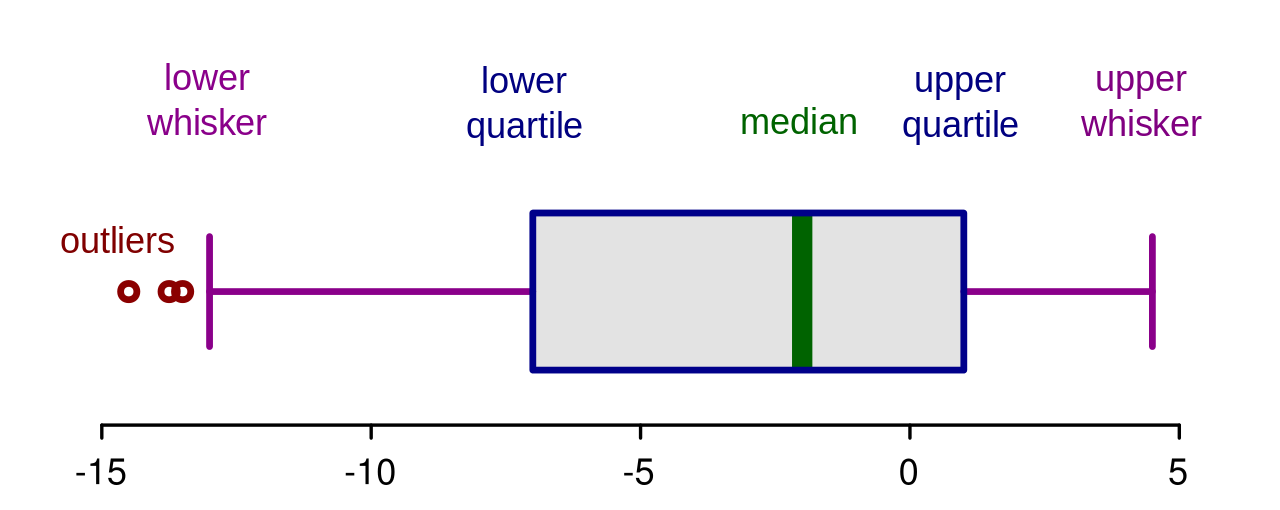
\includegraphics[width=\textwidth,trim={0.5cm .5cm 0.5cm 6cm},clip]{P03box.png}
			\credits{By Ruediger85 at Wikipedia Commons. CC BY-SA 3.0.}
		\end{fig}
	\subsubsection{Pie charts}
		Pie charts are a useful tool to display the shares of different categories. However, they only work out well for relative values and can have a lack of clarity if many small values are included.		
%		\begin{fig}[Pie chart]{fig:pie}{!h}
%			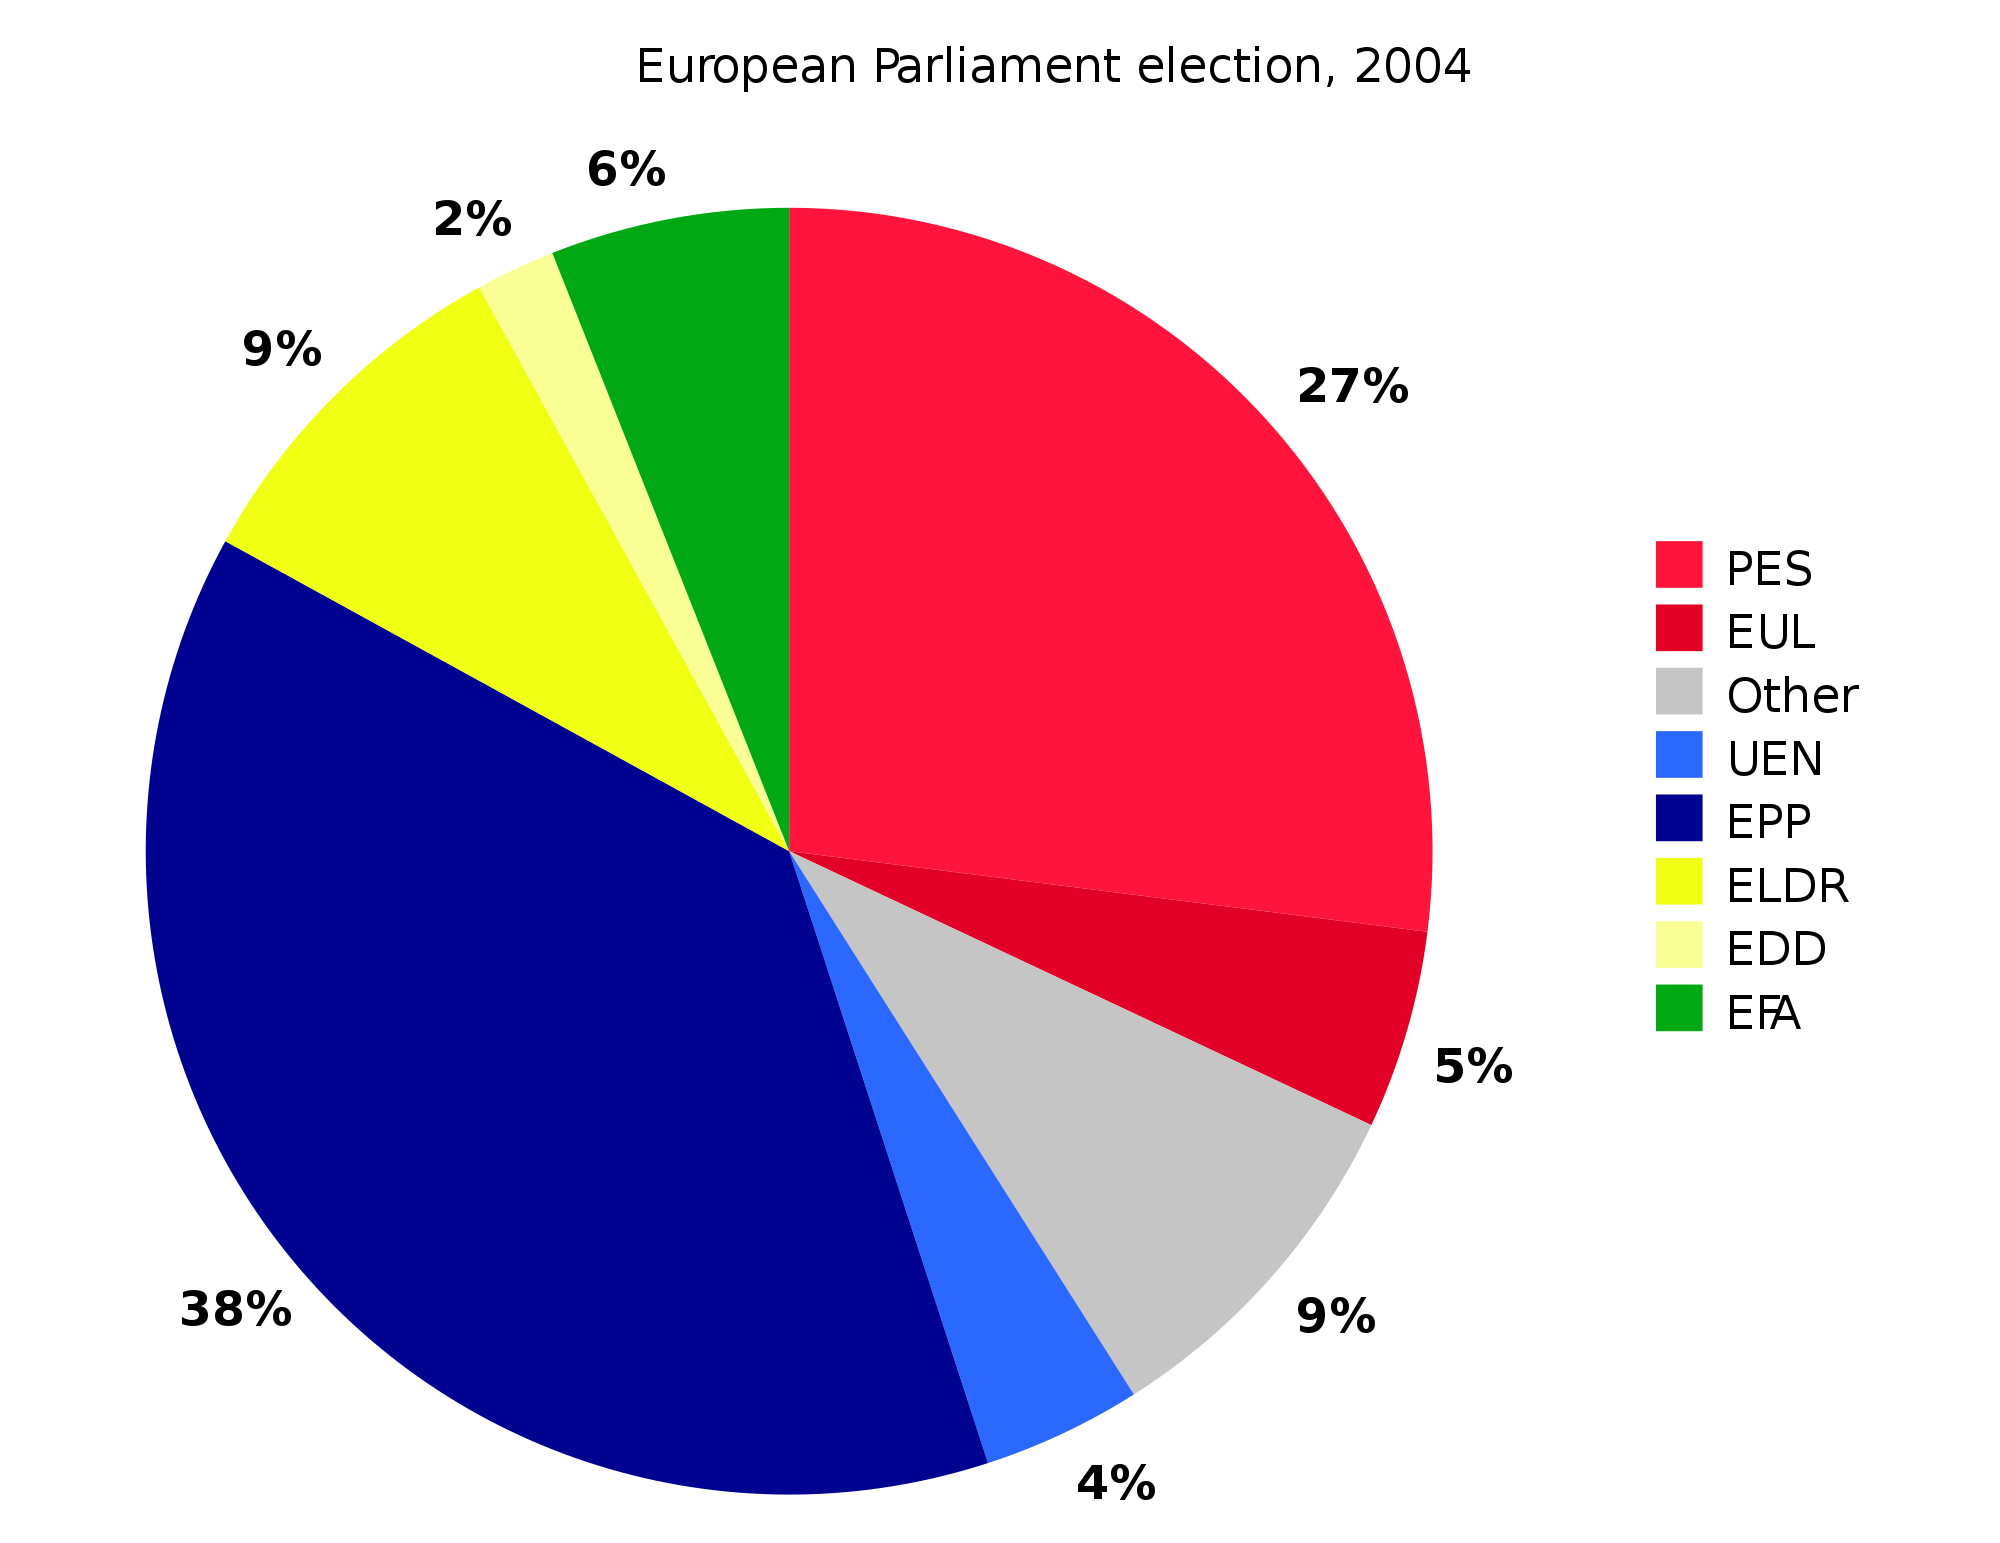
\includegraphics[width=\textwidth,trim={1cm .5cm 3cm 4cm},clip]{P04pie.png}
%			\credits{By Liftarn at Wikipedia Commons. Public Domain.}
%		\end{fig}
	\subsubsection{Scatter plots}
		Scatter plots as in \ref{fig:scatter} display datapoints in a Cartesian coordinate system. This can be done in one to three dimensions, but it is mostly common in two dimensions. Another variable can be displayed by adding color or symbol coding. Scatter plots are helpful to find clusters and get a general idea of how the distribution of the data looks like.				
		\begin{fig}[Scatter plot]{fig:scatter}{!htb}
			\centering{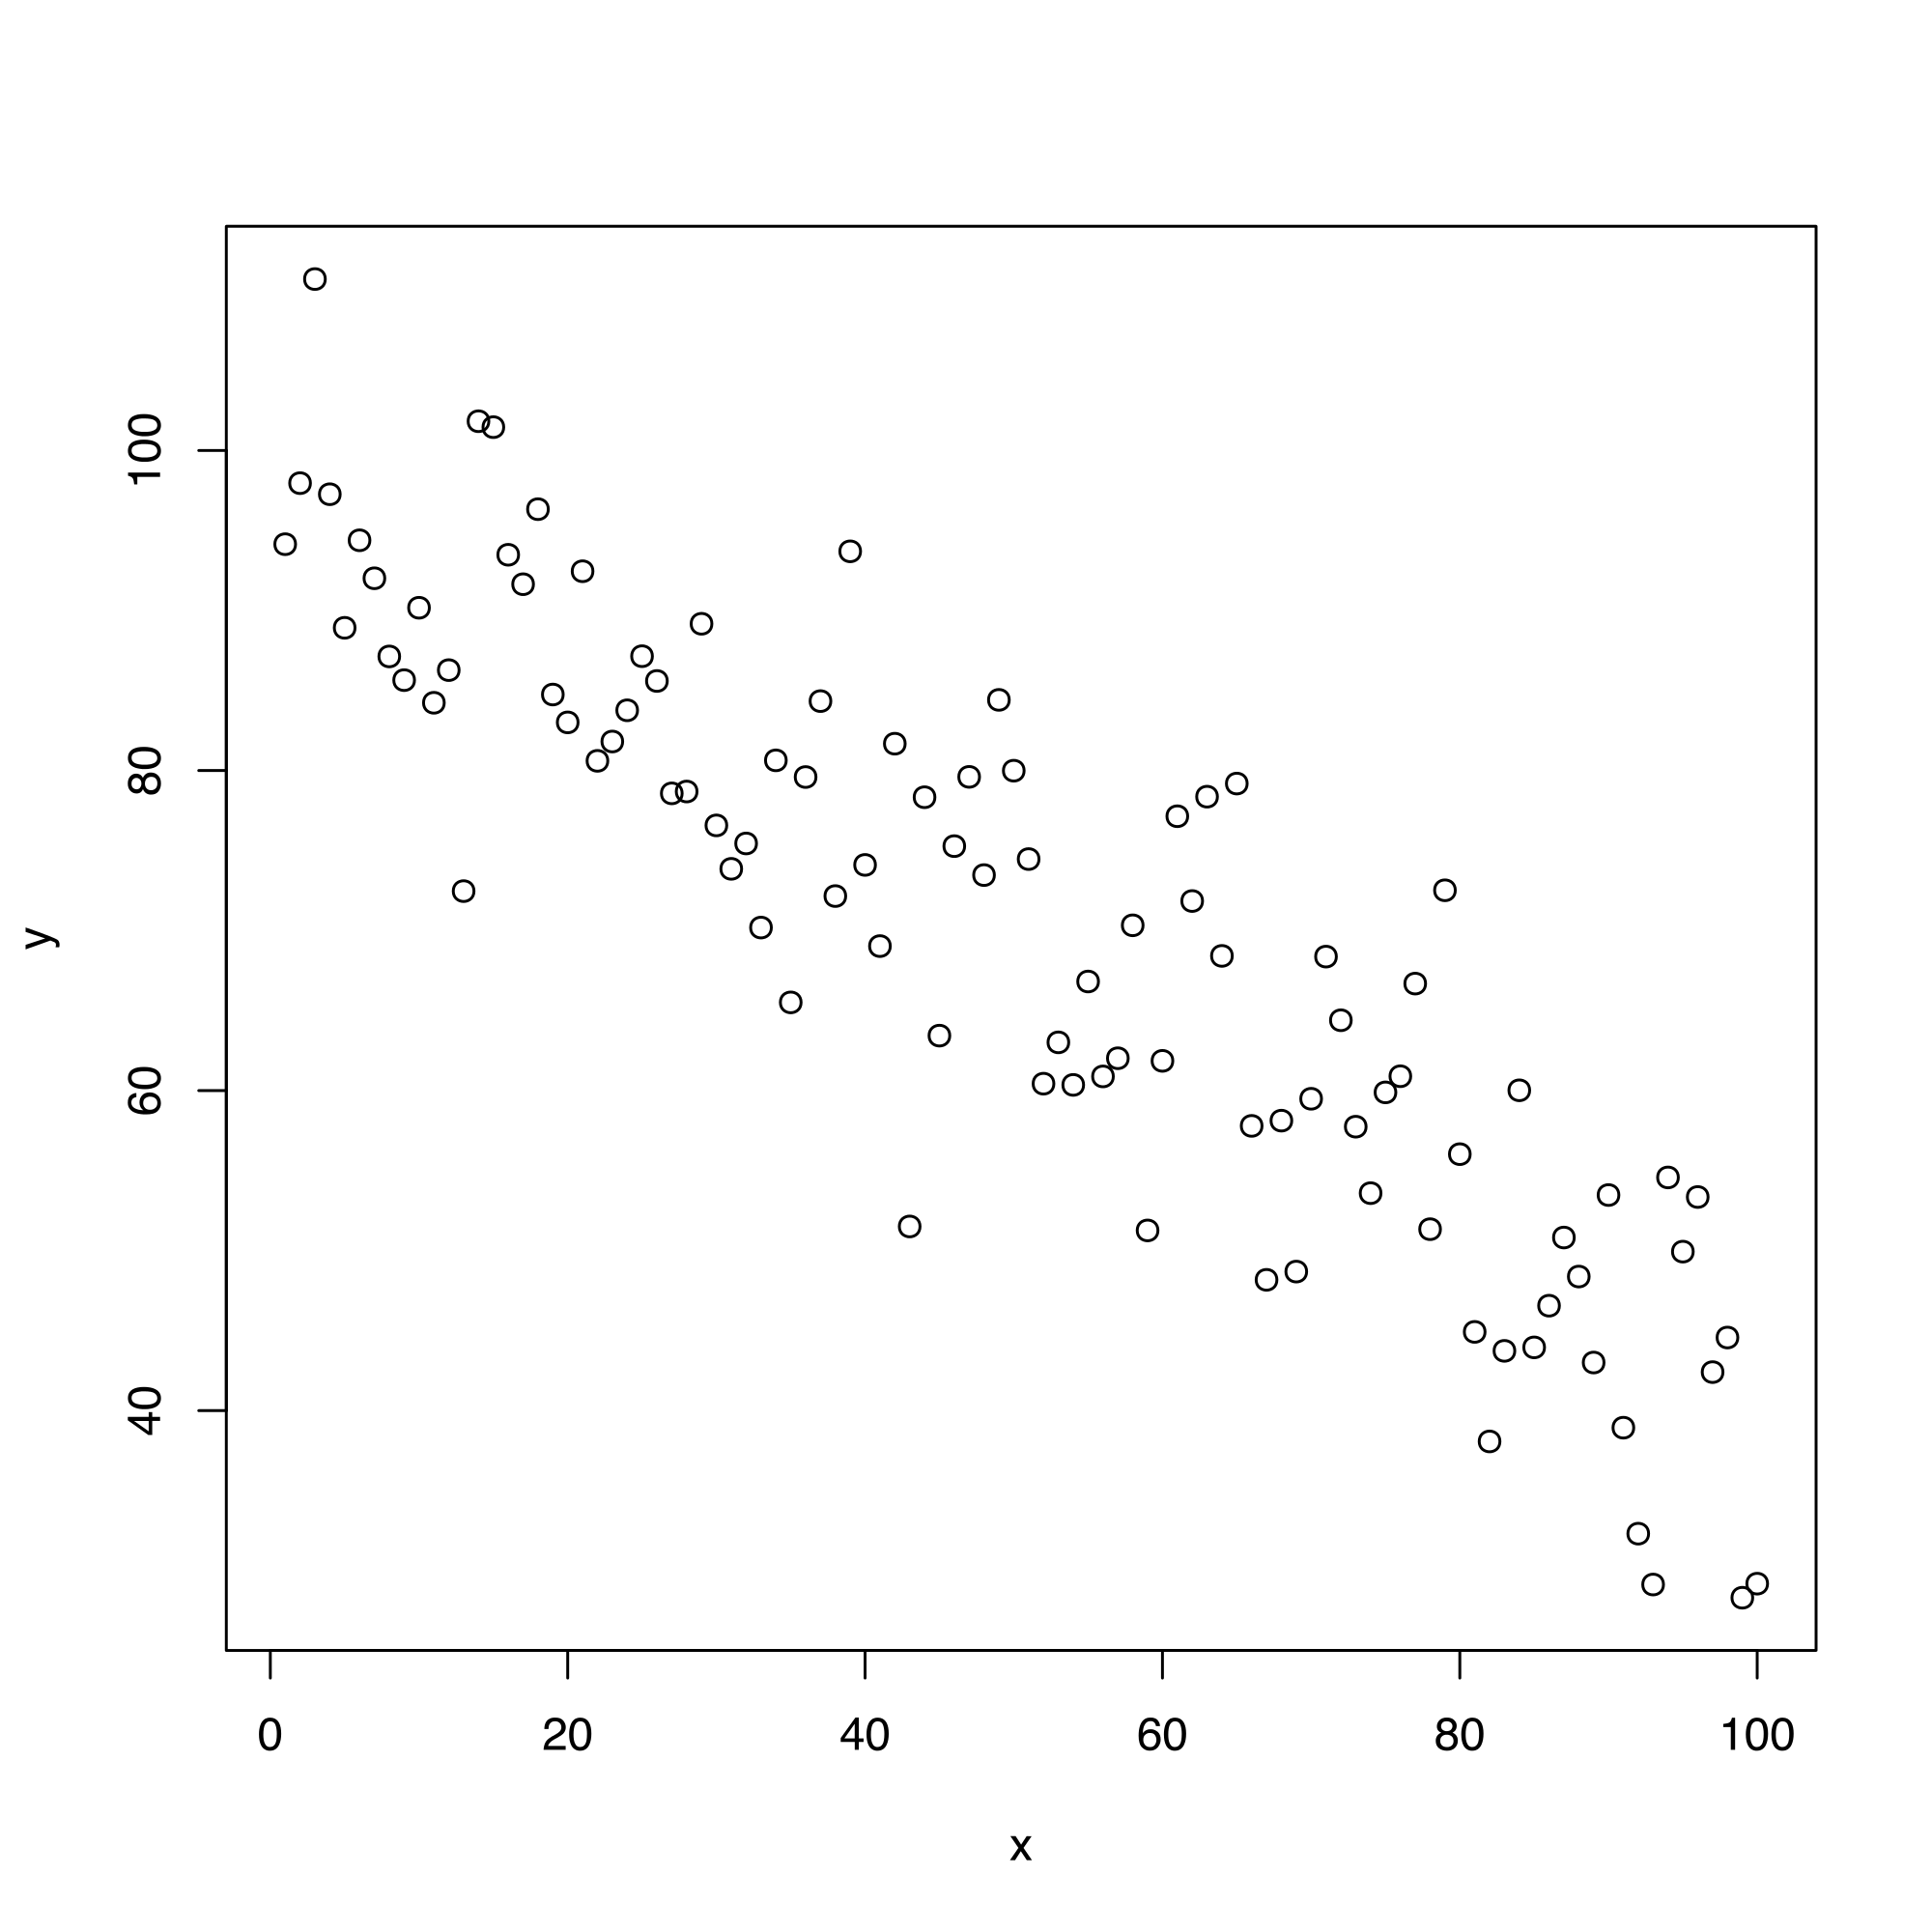
\includegraphics[trim={1cm 2cm 3cm 7cm},clip,width=0.7\textwidth]{P05scatter.png}}
			\credits{By Stiegenaufgang at Wikipedia Commons. CC BY-SA 3.0.}
		\end{fig}				
	\subsubsection{Radar charts}
		Radar charts, also known as spider plots, are shown in figure \ref{fig:radar}. These kind of plots are useful to display how multiple variables changes in different datasets.	This can be helpful to find clusters or outliers in a dataset.								
		\begin{fig}[Spider plot]{fig:radar}{!htb}
			\centering{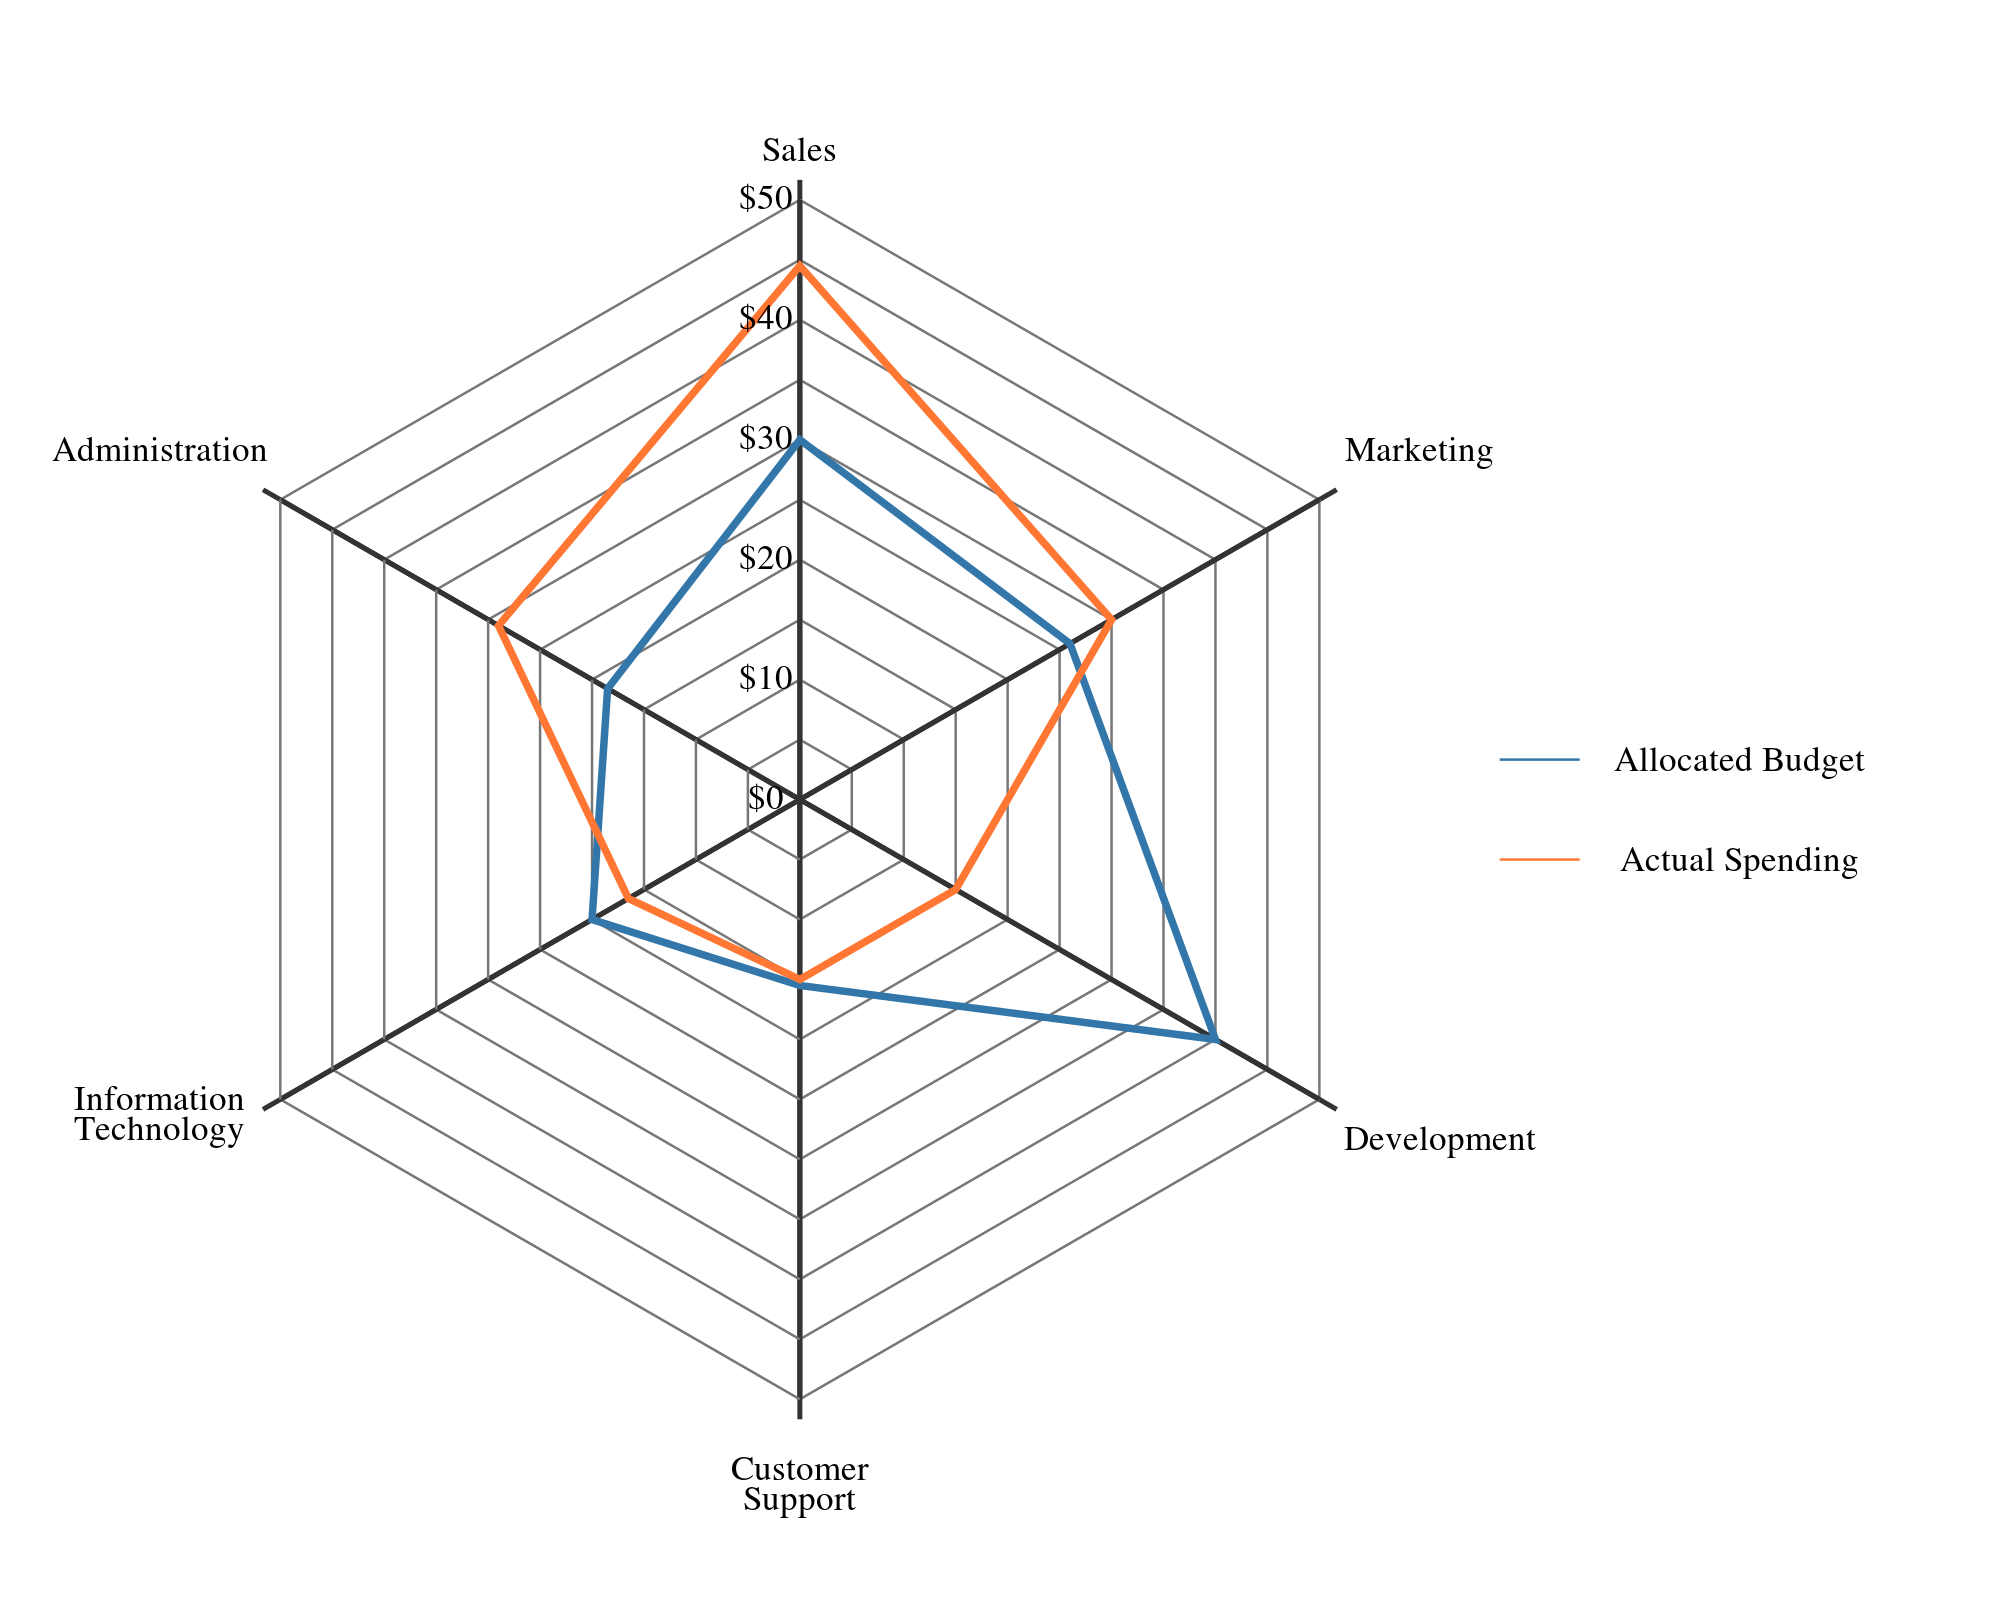
\includegraphics[width=0.7\textwidth,trim={3cm 4.5cm 4.5cm 5.5cm}]{P06radar.png}}
			\credits{Public Domain.}
		\end{fig}		
\subsection{Properties of Estimators}
	Estimators as described in definition \ref{defi:estimator} are important to make statements about the population from a sample. There are many ways to create estimates, and some deliver better results than others.There are some properties that are important for an estimator to be a good estimator.
	\subsubsection{Unbiasedness}
		An estimator is \emph{unbiased} if its expected value is the value of the population parameter of interest $\Theta$. In figure \ref{fig:bias}, the estimator $T_1$ is unbiased because $E(T_1)=\Theta$. The estimator $T_2$ has a bias which is the deviation of its expected value to the population parameter of interest.
		\begin{exmp}[Unbiased Estimator of the population mean]{exmp:bias}
			Consider a random sample
			\begin{equation*}
				\bar{x}=\frac{\sum\limits_{i=1}^n x_i}{n}
			\end{equation*}
			generated by $x_1,x_2,...,x_n$ where the $x_i$ have the same distribution $E(x_i)=\mu$.
			\begin{equation*}
			E\left(\bar{x}\right)=E\left(\frac{\sum\limits_{i=1}^n x_i}{n}\right)=\frac{1}{n} \sum\limits_{i=1}^n E\left(x_i\right)=\frac{1}{n} \sum\limits_{i=1}^n \mu=\frac{n\mu}{n}=\mu
			\end{equation*}
		\end{exmp}
		\begin{fig}[Unbiasedness of an Estimator]{fig:bias}{!htb}
			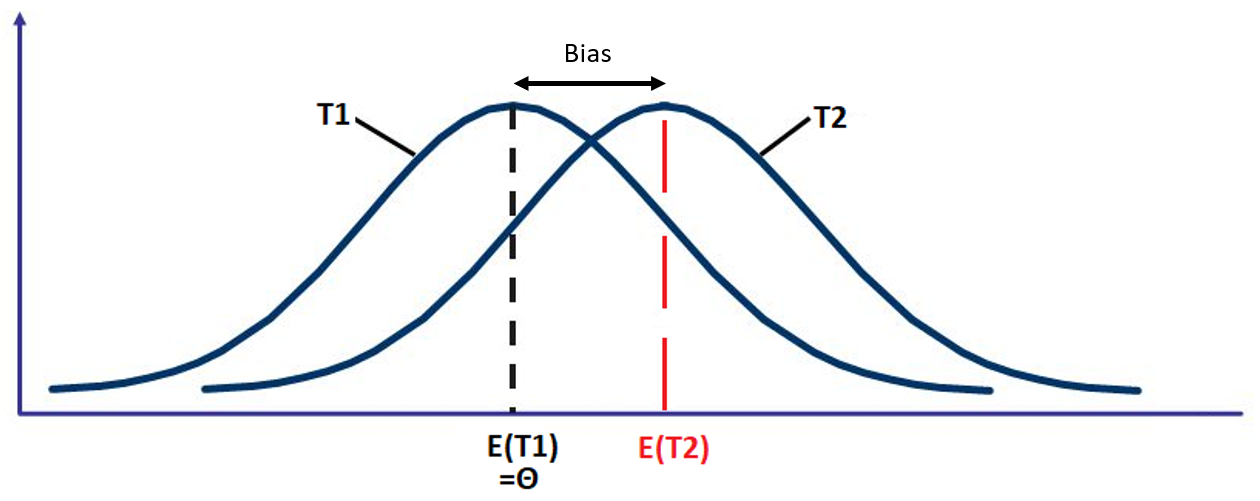
\includegraphics[width=\textwidth]{P07bias.png}
		\end{fig}
	\subsubsection{Efficiency}
		Consider two unbiased estimators $T_1,T_2$ of the same population parameter $\Theta$. $T_1$ is more \emph{efficient} than $T_2$ because if it has a smaller variance as shown in \ref{fig:efficiency}.
		\begin{fig}[Efficiency of an Estimator]{fig:efficiency}{!htb}
			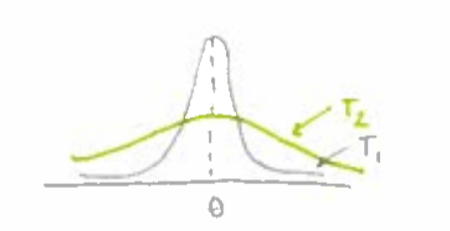
\includegraphics[width=\textwidth,trim={0cm 0cm 0cm .5cm},clip]{P08efficiency.png}
		\end{fig}		
	\subsubsection{Consistency}
		An estimator is \emph{consistent} if the probability that it generates estimates with a small error compared to the population parameter of interest increases to 1 as the sample size becomes infinitely large as shown in figure \ref{fig:consistency}.
		\begin{equation*}
			\forall\,\varepsilon > 0,\qquad \lim\limits_{n\rightarrow+\infty}P_s(|\hat{\Theta}_n-\Theta|>\varepsilon)=0
		\end{equation*}
		with $\hat{\Theta}_n$ as the value of an estimate for $\Theta$ when the sample size is $n$.
	\subsubsection{Sufficiency}
		An estimator is \emph{sufficient} if it contains all information in a sample about the population parameter of interest.
	\subsubsection{Trade-off between unbiasedness and efficiency}
		For an estimator, unbiasedness is desirable but not the only crucial factor. In figure \ref{fig:mse}, we need to decide whether $T_1$ or $T_2$ is the better estimator. This can be determined by calculating the \emph{mean squared error (MSE)}, and the estimator delivering the smallest MSE is the best.
		\begin{equation*}
			MSE(T_1)=var(T)+bias\left(E(T),\Theta\right)
		\end{equation*}
		\begin{fig}[Consistency of an Estimator]{fig:consistency}{!htb}
			\includegraphics[width=\textwidth,trim={0cm 0cm 0.5cm .5cm},clip]{P09Consistency.png}
		\end{fig}			
		\begin{fig}[Mean Square Error an Estimator]{fig:mse}{!htb}
			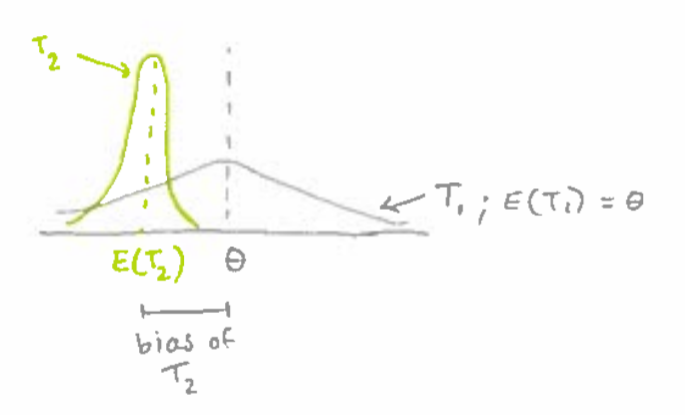
\includegraphics[width=\textwidth]{P10mse.png}
		\end{fig}			
	\subsubsection{Central Limit Theorem (CLT)}\label{sec:clt}
		Consider a sequence of random variables $x_1,x_2,...,x_n$ which are independent identically distributed (i.i.d.) such that $E(x_i)=\mu,\,var(x_i)=\sigma^2$. We are interested in the random variable
		\begin{equation*}
			s_n=\frac{\sum\limits_{i=1}^n x_i}{n}.
		\end{equation*}
		The CLT states that as $n\rightarrow+\infty$ $s_n$ becomes approximately normally distributed with mean $\mu$ and variance $\frac{\sigma^2}{n}$.
		\begin{equation*}
			\sqrt{n}(s_n-\mu)\xrightarrow{d}N(0,\sigma^2),\qquad \xrightarrow{d}\text{ indicates in distribution.}
		\end{equation*}
		Important information we get from this:
		\begin{itemize}
			\item The variance of $s_n$ decreases linearly with $n$, and
			\item $s_n$ is approximately normally distributed with mean $\mu$, so it is \emph{unbiased}.
		\end{itemize}

\section{Statistical Inference}
%%%%%%%%%%%%%%%%%%%%%%%%%%%%%%%%
	\emph{Statistical Inference} is about generating and interpreting confidence intervals and setting up and testing hypotheses. Examples for questions in the field of transportation:
	\begin{itemize}
		\item Do traffic calming measures reduce speed?
		\item Did the deregulation of the airline industry impact the safety of flying?
		\item Do changeable message signs (CMS) reduce the occurrence of secondary incidents?
	\end{itemize}
\subsection{Confidence Intervals (CI)}
	Unknown parameters of the population are not known with full certainty. Working with \emph{confidence intervals} allows to quantify the degree of uncertainty around these parameters.
	\subsubsection{CI for the population mean with known standard deviation}
		When $\sigma$ is known, we can set up a confidence interval for $\mu$ using the CCT (\ref{sec:clt}). If a sample is large enough, then approximately $\bar{x}\sim N(\mu,\frac{\sigma^2}{N})$. So, for approximately normal distributed data, for $\alpha\epsilon(0,1)$, a CI with confidence level $\alpha$ is $\left[\bar{x}-z_{\frac{\alpha}{2}}\frac{\sigma}{\sqrt{n}},\,\bar{x}+z_{\frac{\alpha}{2}}\frac{\sigma}{\sqrt{n}}\right]$ with $n$ as the sample size.
		\begin{fig}[CI for the population mean with known standard deviation]{fig:ci1}{h}
			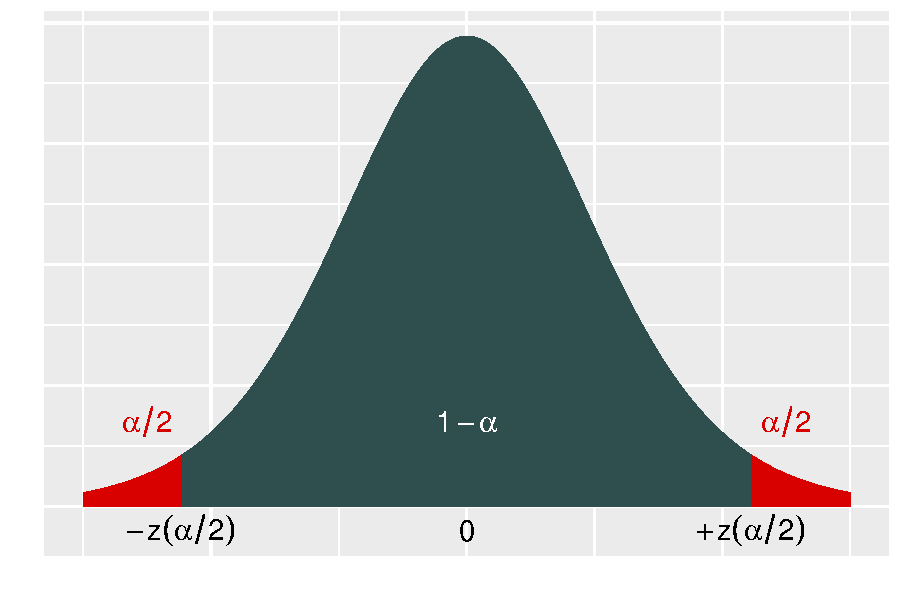
\includegraphics[width=\textwidth]{P11ci.pdf}	
			\credits{By ARAKI Satoru at Wikipedia Commons. CC BY-SA 4.0. Edited.}							
		\end{fig}
	\subsubsection{CI for the population mean with unknown standard deviation}	
		When $\sigma$ is unknown, the notation for the confidence interval changes because we will use the sample's standard error $s$ as an estimator for $\sigma$.
		\begin{equation*}
			CI(\alpha)=\left[\bar{x}-t_{\frac{\alpha}{2}}\frac{s}{\sqrt{n}},\,\bar{x}+t_{\frac{\alpha}{2}}\frac{s}{\sqrt{n}}\right]
		\end{equation*}
		\begin{fig}[CI for the population mean with unknown standard deviation]{fig:ci2}{h}
			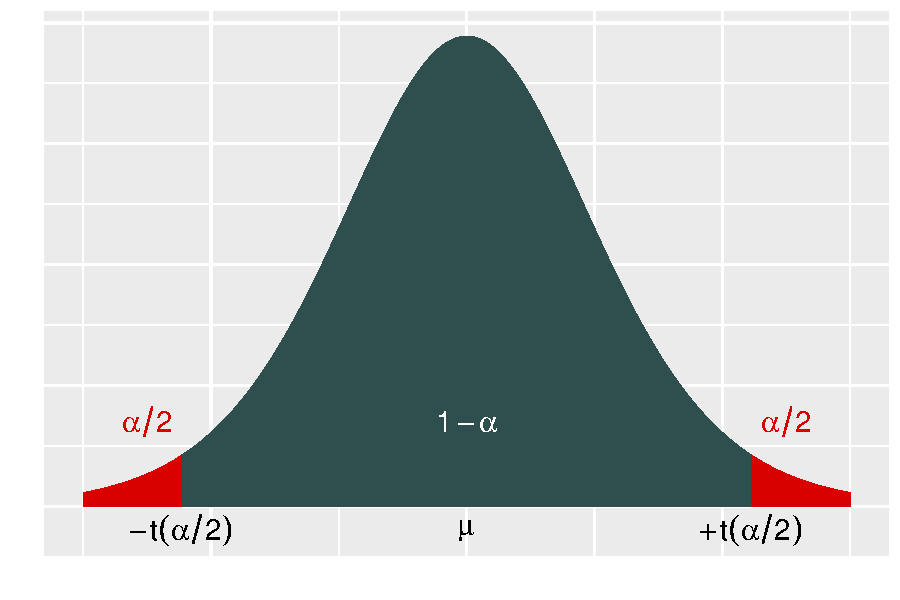
\includegraphics[width=\textwidth]{P12ci.pdf}
			\credits{By ARAKI Satoru at Wikipedia Commons. CC BY-SA 4.0. Edited.}			
		\end{fig}	
	\subsubsection{CI for a population proportion}	
		We can use a sample estimate $\hat{p}$ for a population proportion, e.g. to find out the true percentage of commuters who carpool.
		\begin{equation*}
			CI(\alpha)=\left[\hat{p}-z_{\frac{\alpha}{2}}\sqrt{\frac{\hat{p}(1-\hat{p})}{n}},\hat{p}+z_{\frac{\alpha}{2}}\sqrt{\frac{\hat{p}(1-\hat{p})}{n}}\right]
		\end{equation*}
		Valid if $n_p\geq 5 \bigwedge n(1-p)\geq 5$. Based on the assumption that approx. $\hat{p}\sim N\left(p,\frac{p(1-p)}{n})\right)$.
	\subsubsection{CI for the variance of a population}	
		The test for variances can be used for example to find out whether high speed differences are linked to accidents occurring. Given $\alpha\epsilon(0,1),\,\alpha(1-\alpha)\%$ CI for $\sigma^2$ is:
		\begin{equation*}	
			CI(\alpha)=\left[\frac{(n-1)s^2}{\chi^2_{\frac{\alpha}{2},n}},\frac{(n-1)s^2}{\chi^2_{1-\frac{\alpha}{2},n}}\right]
		\end{equation*}
		\begin{fig}[CI for the variance of a population]{fig:chisq}{h}
			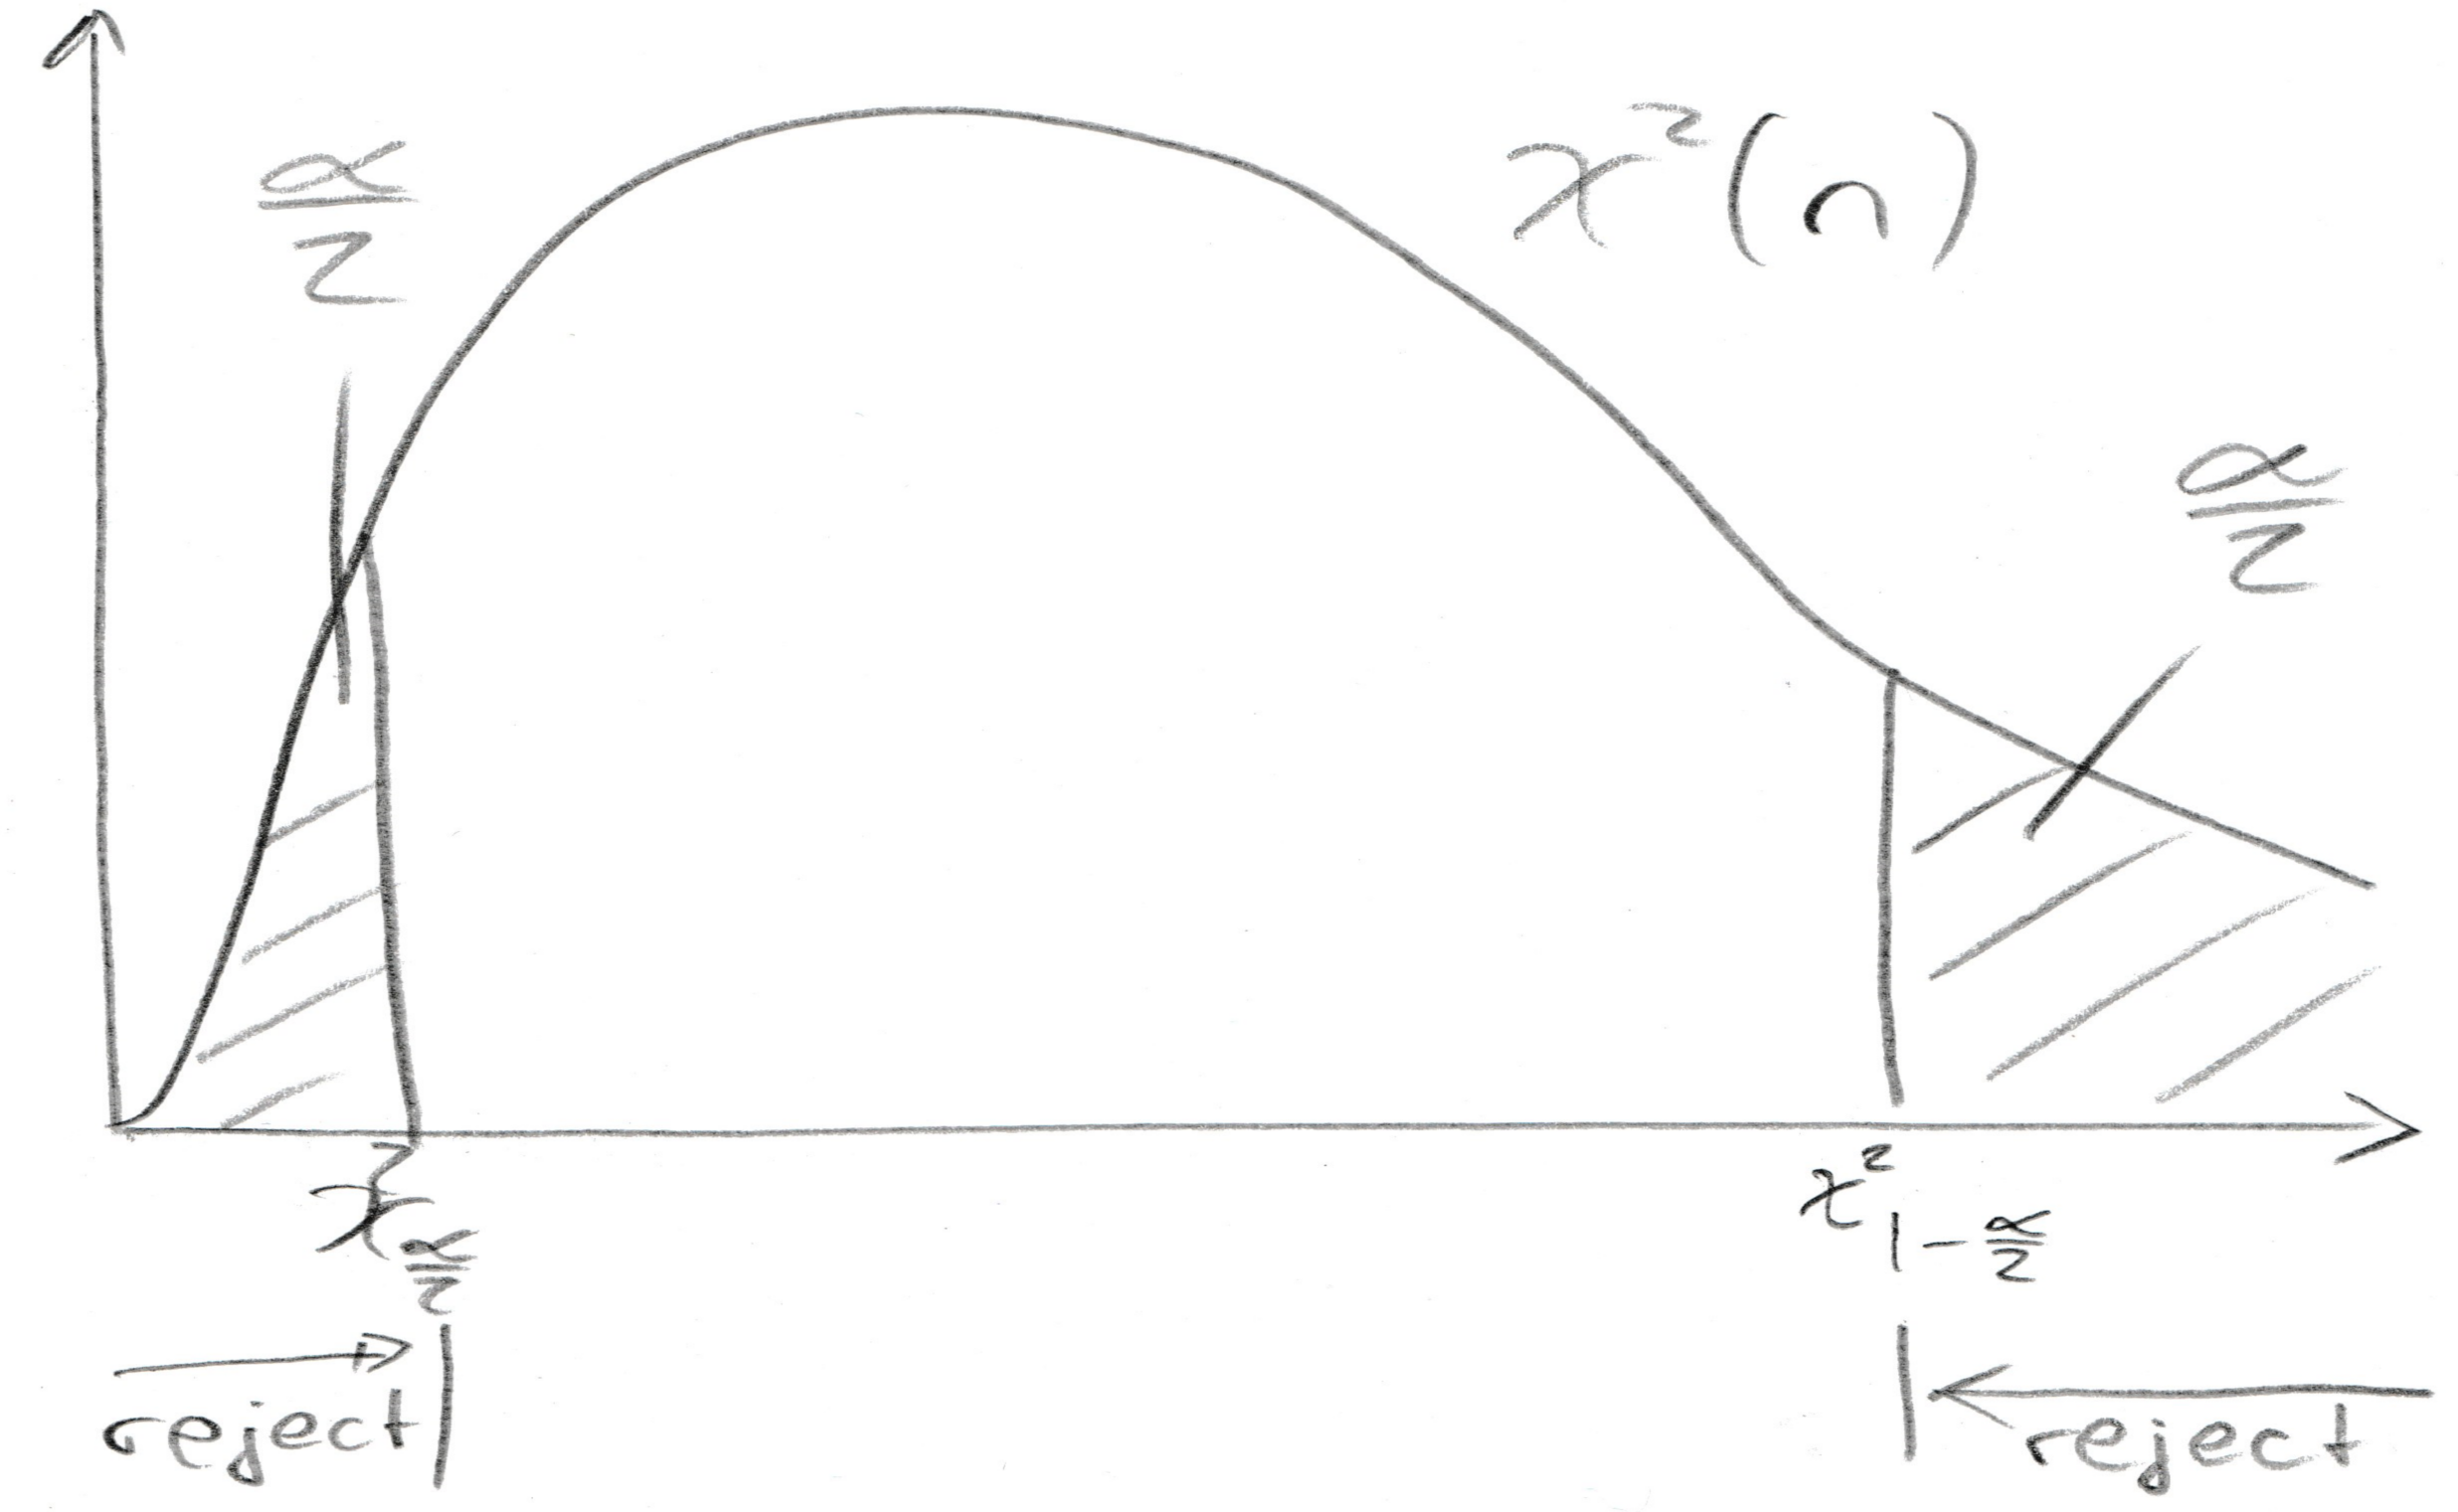
\includegraphics[width=\textwidth]{P14chisq.png}
		\end{fig}			

\subsection{Hypothesis Testing}
	With \emph{hypothesis testing}, we can assess if the value for a parameter we got from an estimator differs from a set value by chance because it is truly different, so it is not related to the actual value of interest. The case of no relation existing is called \emph{null hypothesis}. Hypothesis testing always follows the same framework of the following three steps: 
	\begin{enumerate}
		\item Formulate a null hypothesis $H_0$ and an alternative hypothesis $H_1$ or $H_a$.
		\item Pick a test statistic (a function based on the sample data) which helps to decide between $H_0$ and $H_1$, and gives a distribution if $H_0$.
		\item Calculate the test statistic, pick a probability $\alpha$ of being wrong if $H_0$ is true, \enquote{a burden of proof}. State and apply a decision rule (i.e. a rejection region). Conclude the results clearly.
	\end{enumerate}
	Depending of the question the test is carried out for, $H_0$ can be described with an $=,\,\leq,$ or $\geq$ sign. $H_1$ is the negated version of $H_0$, so not less or equal which means greater than. The mentioned distribution of the test statistic usually will be Normal ($N$), $F(p,q)$ or Chi-Squared ($\chi^2(n)$). The results can either indicate that we have to \emph{reject} $H_0$, or if we cannot confirm that the null hypothesis is wrong, we \emph{fail to reject it}.
	\begin{defi}[Errors in hypothesis testing]{defi:hyperror}
		There are two types of errors which occur when conducting hypothesis testing.
		\centering{
			\begin{tabular}{p{0.2\linewidth}|p{0.35\linewidth}|p{0.35\linewidth}}
				actual truth $\rightarrow$ test result $\downarrow$ & $H_0$ is true & $H_0$ is false\\\hline
				reject $H_0$ & Type I error. Control error size by choosing $\alpha$. & OK\\\hline
				fail to reject $H_0$ & OK & Type II error. $P\sim(E_{II})=\beta$.
			\end{tabular}
		}
	\end{defi}
	\begin{exmp}[Hypothesis statements]{exmp:hypstate}
		We want to asses whether increasing the landing fees at John-Wayne Airport (SNA) has an impact on the number of monthly flights as SNA?
		\begin{enumerate}
			\item $N=\#$flights at SNA. Current $\#$flights is $N_0$.
				\begin{equation*}
					H_0:\;N=N_0\qquad vs. \qquad H_1:\;N\neq N_0
				\end{equation*}
			\item Will a 10\% increase in landing fees show in a decrease in $\#$flights?
				\begin{equation*}
				H_0:\;N\geq N_0\qquad vs. \qquad H_1:\;N<N_0
				\end{equation*}
		\end{enumerate}
	\end{exmp}
	\subsubsection{Interference about a single population}
		We assume that the samples we have come from approximately normal distributed populations. The results are robust against \emph{small} deviations from this assumption in reality.
		\myparagraph{Test a population mean with unknown variance}
			\begin{enumerate}
				\item State $H_0$ and $H_1$ context specific.
				\item Pick the test statistic $T^*=\frac{\bar{x}-\mu_0}{s/\sqrt{n}}$. If $H_0$ is true, $T^*\sim t(n-1)$.
				\item Calculate $T^*$. Pick the confidence level (and probability for a type I error) $\alpha$. Common values for $\alpha$ are 0.5\%, 1\%, 5\%, or 10\%.
			\end{enumerate}
			The idea is to reject $H_0$ if the observation is highly unlikely to be based on this hypothesis.
			\begin{exmp}[One- and two-tailed hypothesis tests]{exmp:tails}
				One-tailed: $H_0:\;\mu=\mu_0\; vs. \; H_1:\;\mu\neq\mu_0$\hfill Two-tailed: $H_0:\;\mu\geq\mu_0\; vs. \; H_1:\;\mu<\mu_0$
				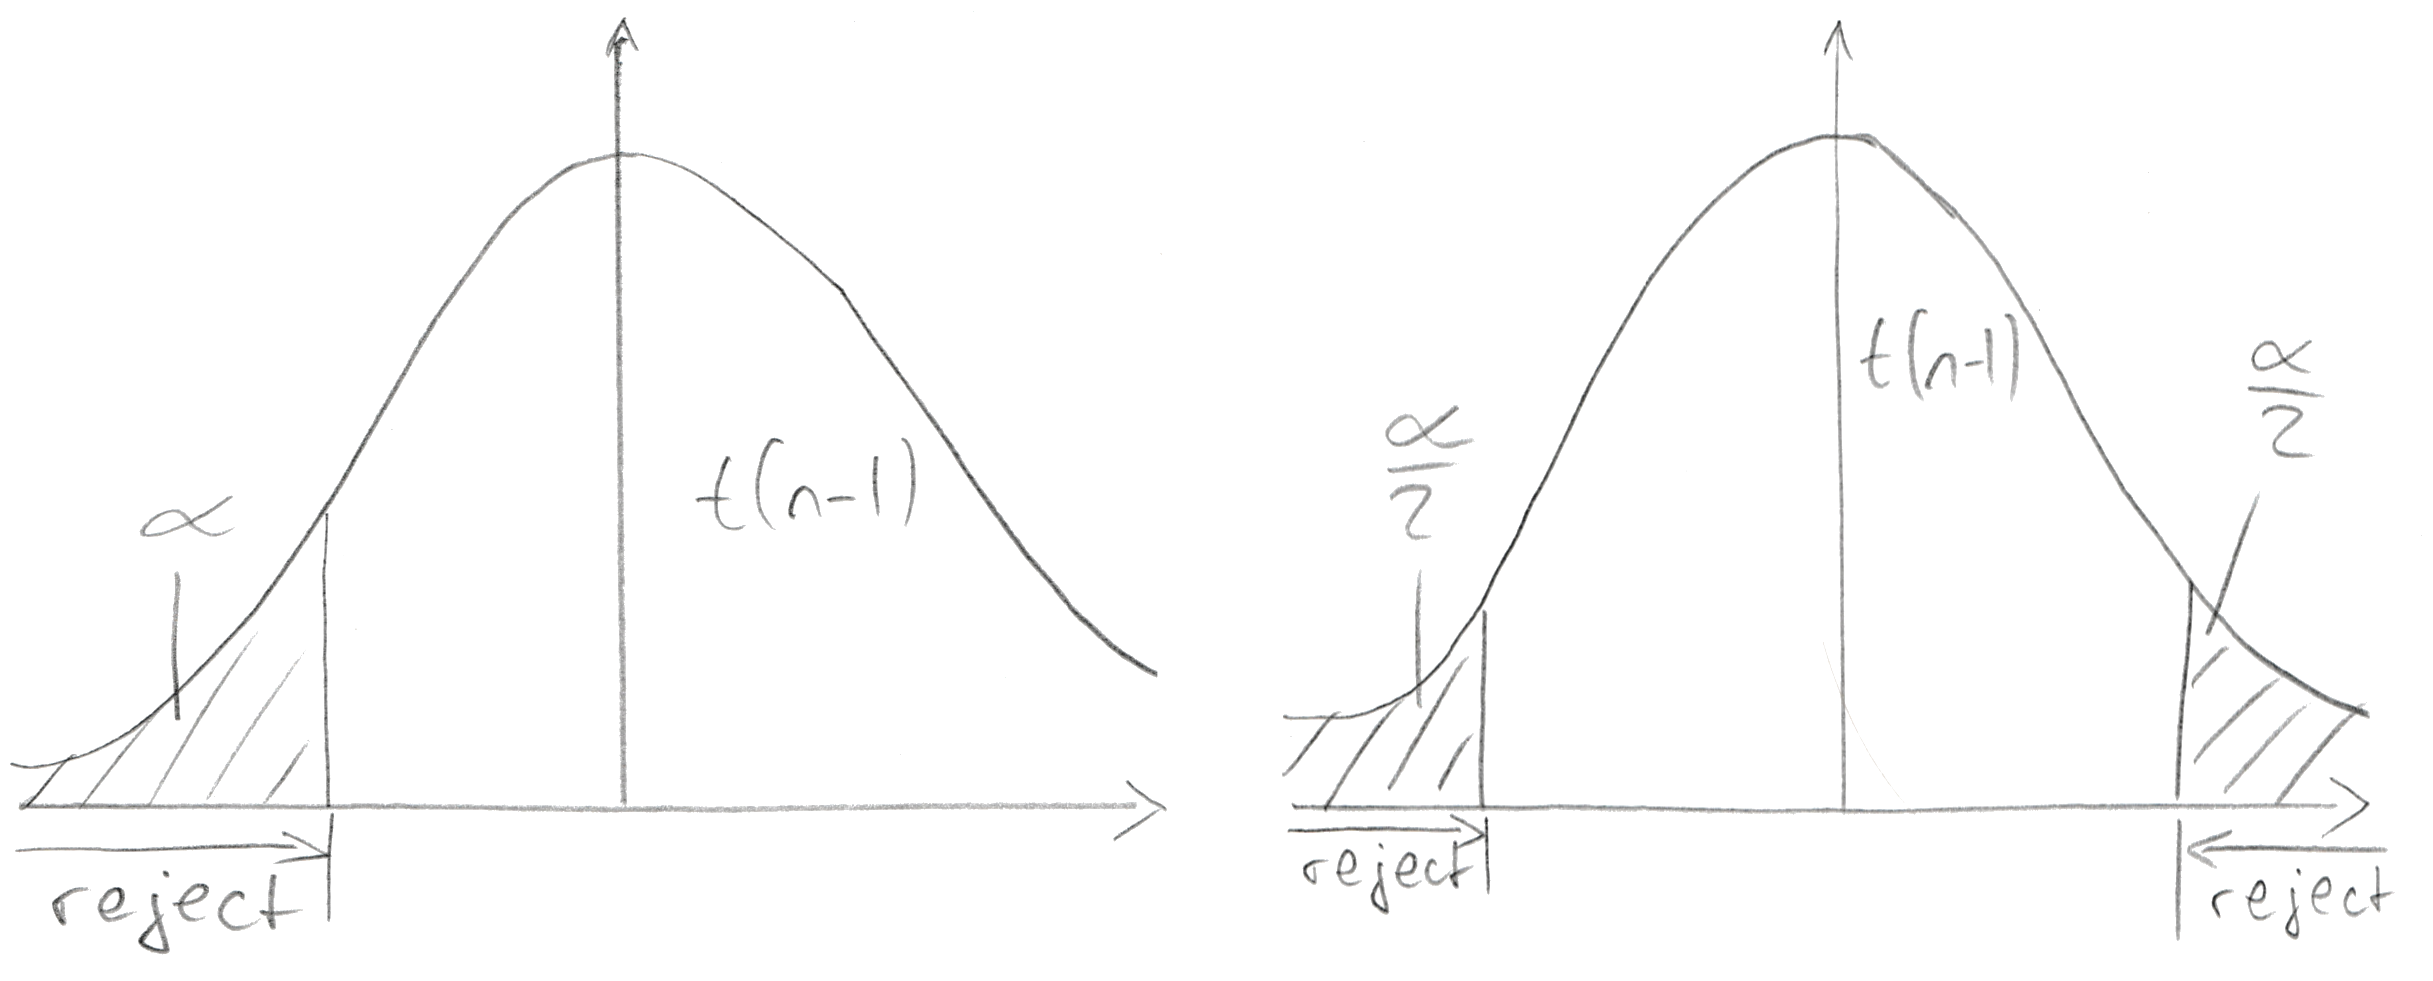
\includegraphics[width=\textwidth]{P15-16-tails.png}
			\end{exmp}
		\myparagraph{Test a population variance}	
			The same 3-step-framework is used. For testing a null hypothesis of $\sigma_0^2$ from a sample size $n$, the test statistic is
			\begin{equation*}
				\chi^2=\frac{(n-1)s^2}{\sigma^2_0}.
			\end{equation*}
			If $H_0$ is true, $\chi^2\sim\chi^2(n-1)$.
			\begin{exmp}[Hypothesis testing for variance]{exmp:vartest}
				Testing if the variance of vehicle speeds on the I-405 on weekday afternoons equal to $10 MPH^2$? We have a random sample with $n=100$ from which we calculate $s^2=9 MPH^2$.
				\begin{enumerate}
					\item $H_0:\;\sigma^2=\sigma^2_0=10 MPH^2 \qquad vs. \qquad H_1\sigma^2\neq 10 MPH^2$
					\item $\chi^2=\frac{(n-1)s^2}{\sigma_0^2},\; \chi^2\sim\chi^2(n-1)$
					\item $\alpha=5\%=0.05,\; \chi^2=\frac{99\cdot9}{10}=89.1$ This value is within the confidence interval of $\left[73.36,128.42\right]$. Therefore, we fail to reject the null hypothesis.
				\end{enumerate}
			\end{exmp}
		\myparagraph{Test a population proportion}	
			We use the same framework to test if a population has a certain proportion $p$. The following $z$ test statistic is used:
			\begin{equation*}
				Z^*=\frac{\hat{p}-p_0}{\sqrt{\frac{\hat{p}(1-\hat{p})}{n}}}\text{. If $H_0$ is true, }z\sim N(0,1)
			\end{equation*}		
			with $\hat{p}$ as a random variable that gives us the sample proportion, $p_0$ as the proportion specified in $H_0$ and sample size $n$.
	\subsubsection{Comparison of two populations}
		\myparagraph{Compare two means from independent samples}	
			Assume that the CLT (\ref{sec:clt}) applies. Using the same framework, we test for the sample means as estimators of the population mean.
			\begin{equation*}
				Z^*=\frac{\bar{x_1}-\bar{x_2}-(\mu_{01}-\mu_{01})}{\sqrt{\frac{s_1^2}{n_1}+\frac{s_2^2}{n_2}}}
			\end{equation*}
			\begin{exmp}[Hypothesis testing average on-time flights]{exmp:meantest}
				We test if \emph{1: Lufthansa} or \emph{2: Air France} is more on time in average. Therefore, we test for $H_0$ of Lufthansa being more on time.
				\begin{equation*}
					H_0:\;\mu_{10}-\mu_{20}\leq 0\qquad vs. \qquad H_1:\;\mu_1-\mu_2>0
				\end{equation*}
			\end{exmp}
			If $H_0$ is true, for normal and small samples $n_1,n_2\leq 25$, $T\sim t_{dof}$ with $dof$ degrees of freedom (rounded to the next integer).
			\begin{equation*}
				dof=INT\left[\frac{\left(\frac{s_1^2}{n_1}+\frac{s_2^2}{n_2}\right)^2}{\frac{(s_1^2/n_1)^2}{n_1-1}+\frac{(s_2^2/n_2)^2}{n_2-1}}\right]
			\end{equation*}	
			If the populations have the same variances, the following test statistic can be used and compared to a t-distribution with $dof=n_1+n_2-2$.
			\begin{equation*}
				\frac{\bar{x_1}-\bar{x_2}-(\mu_{10}-\mu_{20})}{\sqrt{s^2\left(\frac{1}{n_1}+\frac{1}{n_2}\right)}}
			\end{equation*}
		\myparagraph{Compare two means from paired observations}	
			For two paired datasets of the size $n_d$ and the difference parameters marked by $\bar{x_d},s_d$, we use the following test statistic:
			\begin{equation*}
				T^*=\frac{\bar{x_d}\mu_0}{s_d/\sqrt{n_d}}\text{. If $H_0$ is true, }T^*\sim t(n_d-1)
			\end{equation*}				
		\myparagraph{Evaluate the difference between two population proportions}	
			For large enough sample size, we can test differences as $H_0:\;p_1-p_2=,\leq,\geq p_{d0}$.
			\begin{equation*}
					Z^*=\frac{\hat{p}_1-\hat{p}_2-p_d}{\sqrt{\frac{\hat{p}_1(1-\hat{p}_2)}{n_1}+\frac{\hat{p}_1(1-\hat{p}_2)}{n_2}}}\text{. If $H_0$ is true, }Z^*\sim N(0,1)				
			\end{equation*}
		\myparagraph{Compare two population variances}
			They can be compared using the following f-test:	
			\begin{equation*}
				F^*=\frac{s_1^2}{s_2^2}\text{. If $H_0$ is true, }F^*\sim F(n_1-1,n_2-1)				
			\end{equation*}
		Further information on hypothesis testing can be found in \textcite{Conover.1999} and \textcite[p. 28ff.]{Washington.2011}.		
\begin{famo}[Karl Pearson]{famo:pearson}
		\emph{Karl Pearson} (March 1857 – 27 April 1936) was an English mathematician and biostatistician. He established the discipline of mathematical statistics, and contributed significantly to biometrics, meteorology. Pearson was a protégé and biographer of Sir Francis Galton, who coined the term \enquote{regression}.
	
	After a private education at University College School, he went to King's College, Cambridge in 1876 to study mathematics. He then traveled to Germany to study physics and metaphysics in Heidelberg. He attended lectures on Darwinism, but also Roman law, medieval and 16th century German literature, and Socialism in Berlin.
	
	After returning to London, he studied law until 1881 but never practiced. He then returned to mathematics, first at King's College, London in 1881 and then at University College, London in 1883. After his appointment to the professorship of Geometry at Gresham College, he met Walter Frank Raphael Weldon, a zoologist with whom he developed a fruitful collaboration. Weldon introduced him to Darwin's cousin Francis Galton. Pearson became Galton's protégé, and after Galton's death in 1911, he wrote his biography. He formed the Department of Applied Statistics, into which he incorporated the Biometric and Galton laboratories. In 1890, he married Maria Sharpe, and they had three children. 
	
	Unfortunately, Pearson was racist, anti‐Semitic, and a proponent of eugenics, i.e., a social philosophy advocating the improvement of human genetic traits through the promotion of higher rates of reproduction for people with desired traits, and reduced rates of reproduction and sterilization of people with less‐desired or undesired traits. 

	Pearson's work embraced wide applications and the development of mathematical statistics, with contributions to \emph{biology, epidemiology, anthropometry, medicine, psychology and social history}. In 1901, with Weldon and Galton, he founded the journal Biometrika that focuses on statistical theory. Pearson's thinking underpins many of the 'classical' methods which are in common use today. Some contributions are:
	\begin{itemize}
		\setlength{\itemsep}{0pt}
		\setlength{\parskip}{0pt} 		
		\item Correlation coefficient. He studied its relationship with  linear regression,
		\item method of moments: Pearson introduced the concept borrowed from physics,
		\item Pearson's system of continuous univariate probability distributions that came to form the basis of the now conventional continuous probability distributions,
		\item foundations of hypothesis testing and of the statistical decision theory,
		\item use of P-values and Pearson's chi-squared test,
		\item Principal component analysis. 
	\end{itemize}
	\credits{Source: \url{https://en.wikipedia.org/wiki/Karl_Pearson}}
\end{famo}			
\section{Linear Regression (LR)}
%%%%%%%%%%%%%%%%%%%%%%%%%%%%%%%%
Linear regression is widely used because it is a method which is easy to calculate. Also, linear models are easy to interpret and therefore chosen in many different contexts. However, it is important to remember the underlying assumptions when using LR.
\subsection{Assumptions}\label{sec:ass}
	\begin{exmp}[Linear and non-linear models]{exmp:lin}
		Which of the following models is linear?
		\begin{enumerate}
			\item $y=\alpha_0+\alpha_1 x_1^2+\alpha_2 x_2 + \alpha_3 x_3 + \epsilon$
			\item $y=\alpha x_1^\beta \mu x_2^\gamma$
			\item $y=\alpha_0+\alpha_1 x_1+\alpha_2 x_2 + \eta$
			\item $y=\alpha+\frac{tan\left(\beta x_1 + \gamma x_2^2\right)}{1+2 x_1^3} + \epsilon$
		\end{enumerate}
		Solution:
		\begin{enumerate}
			\item Is linear because all parameters $\alpha$ are linear, the regressors $x$ can be transformed. $\epsilon$ is an error term.
			\item Is non-linear, but can be transformed to a linear model by an easy logarithmic (ln) transformation.
			\item Is linear.
			\item Is non-linear because the parameters are in non-linear form which cannot easily be transformed to a linear function.
		\end{enumerate}		
	\end{exmp}
	\subsubsection{Linearity in the unknown parameters (A1)}\label{sec:ass1}
		The unknown parameters linking the dependent variable $y$ with the known explanatory variables or regressors $x$ have to be linear.  
		\begin{equation*}
			\overbrace{y}^{\hbox{dependent}}_{n\times 1}=\overbrace{x}^{\hbox{regressor}}_{n\times k}\times\overbrace{\beta}^{\hbox{parameter}}_{k\times 1}+\overbrace{\epsilon}^{\hbox{error}}_{n\times 1}
		\end{equation*}
		Where $n=[1,2,...,n]$ is the sample size and $\beta=[0,1,...,k-1]$ are the number parameters we are looking for.
		\begin{align*}
			\begin{cases}
				y_1&=\beta_0+\beta_1 x_{11}+\beta_2 x_{12}+\cdots+\beta_{k-1} x_{1k-1}+\epsilon_1\\
				&\vdots\\
				y_n&=\beta_0+\beta_1 x_{n1}+\beta_2 x_{n2}+\cdots+\beta_{k-1} x_{nk-1}+\epsilon_n
			\end{cases}			
		\end{align*}
	\subsubsection{Unbiasedness of the error term (A2)}		
		The error term consists of random errors and variables that have been excluded in an act of simplifying. However, the error term shall not have any systematic bias but be independently and identically distributed (i.i.d.) for all $\epsilon_i\sim(0,\sigma^2)$ with mean 0 (unbiased) and an unknown variance. This implies that $E(\epsilon_i)=0$.	
	\subsubsection{Homoscedasticity of the error term (A3)}		
		The distribution has the variance $var(\epsilon_i)=\sigma^2 $.	This variance is the same for all observations.
	\subsubsection{Independence of the error term (A4)}	
		The errors of different observations are not related: $cov(\epsilon_i,\epsilon_j)=0\;\forall\;i\neq j$.
	\subsubsection{Exogeneity of the regressors (A5)}
		The values of the explanatory variables or regressors are determined solely by influences \emph{outside} of the environment depicted by the model. This means, $y$ shall not have any direct influence on the value of any $x$.
		\begin{equation*}
			\forall\;(i,j)\varepsilon\left\{0,...,k-1\right\}\times\left\{1,...,n\right\},\quad cov(x_i,\epsilon_j)=0
		\end{equation*}
	\subsubsection{Normal distribution of error terms (A6)}\label{sec:ass6}
		For the purpose of testing the model, we also require the error terms $\epsilon_i$ to be approximately normal distributed.
		\begin{equation*}
			\forall\;(i)\varepsilon\left\{1,...,n\right\},\quad \epsilon_i\sim N(0,\sigma^2)
		\end{equation*}																	
	
	From these assumption we can conclude:
	\begin{equation*}
		y_i\sim N\left((x)_i\beta,\sigma^2\right)
	\end{equation*}
	with $(x)_i$ as the $i^{th}$ row (dimension $1\times k$) of the regressors $x$ and $\beta$ with  dimension $k\times 1$. This means, we assume all $x_{ij}$ are known.
\subsection{Estimation}
	To find estimates for the unknown $\beta$ and $\sigma^2$, we use the method of \emph{linear regression}. It helps to understand how the regressors $x$ affect the dependent variable $y$.	
	\subsubsection{Least Squares}\label{sec:ols}
		\begin{fig}[Ordinary least squares]{fig:ols}{h}
			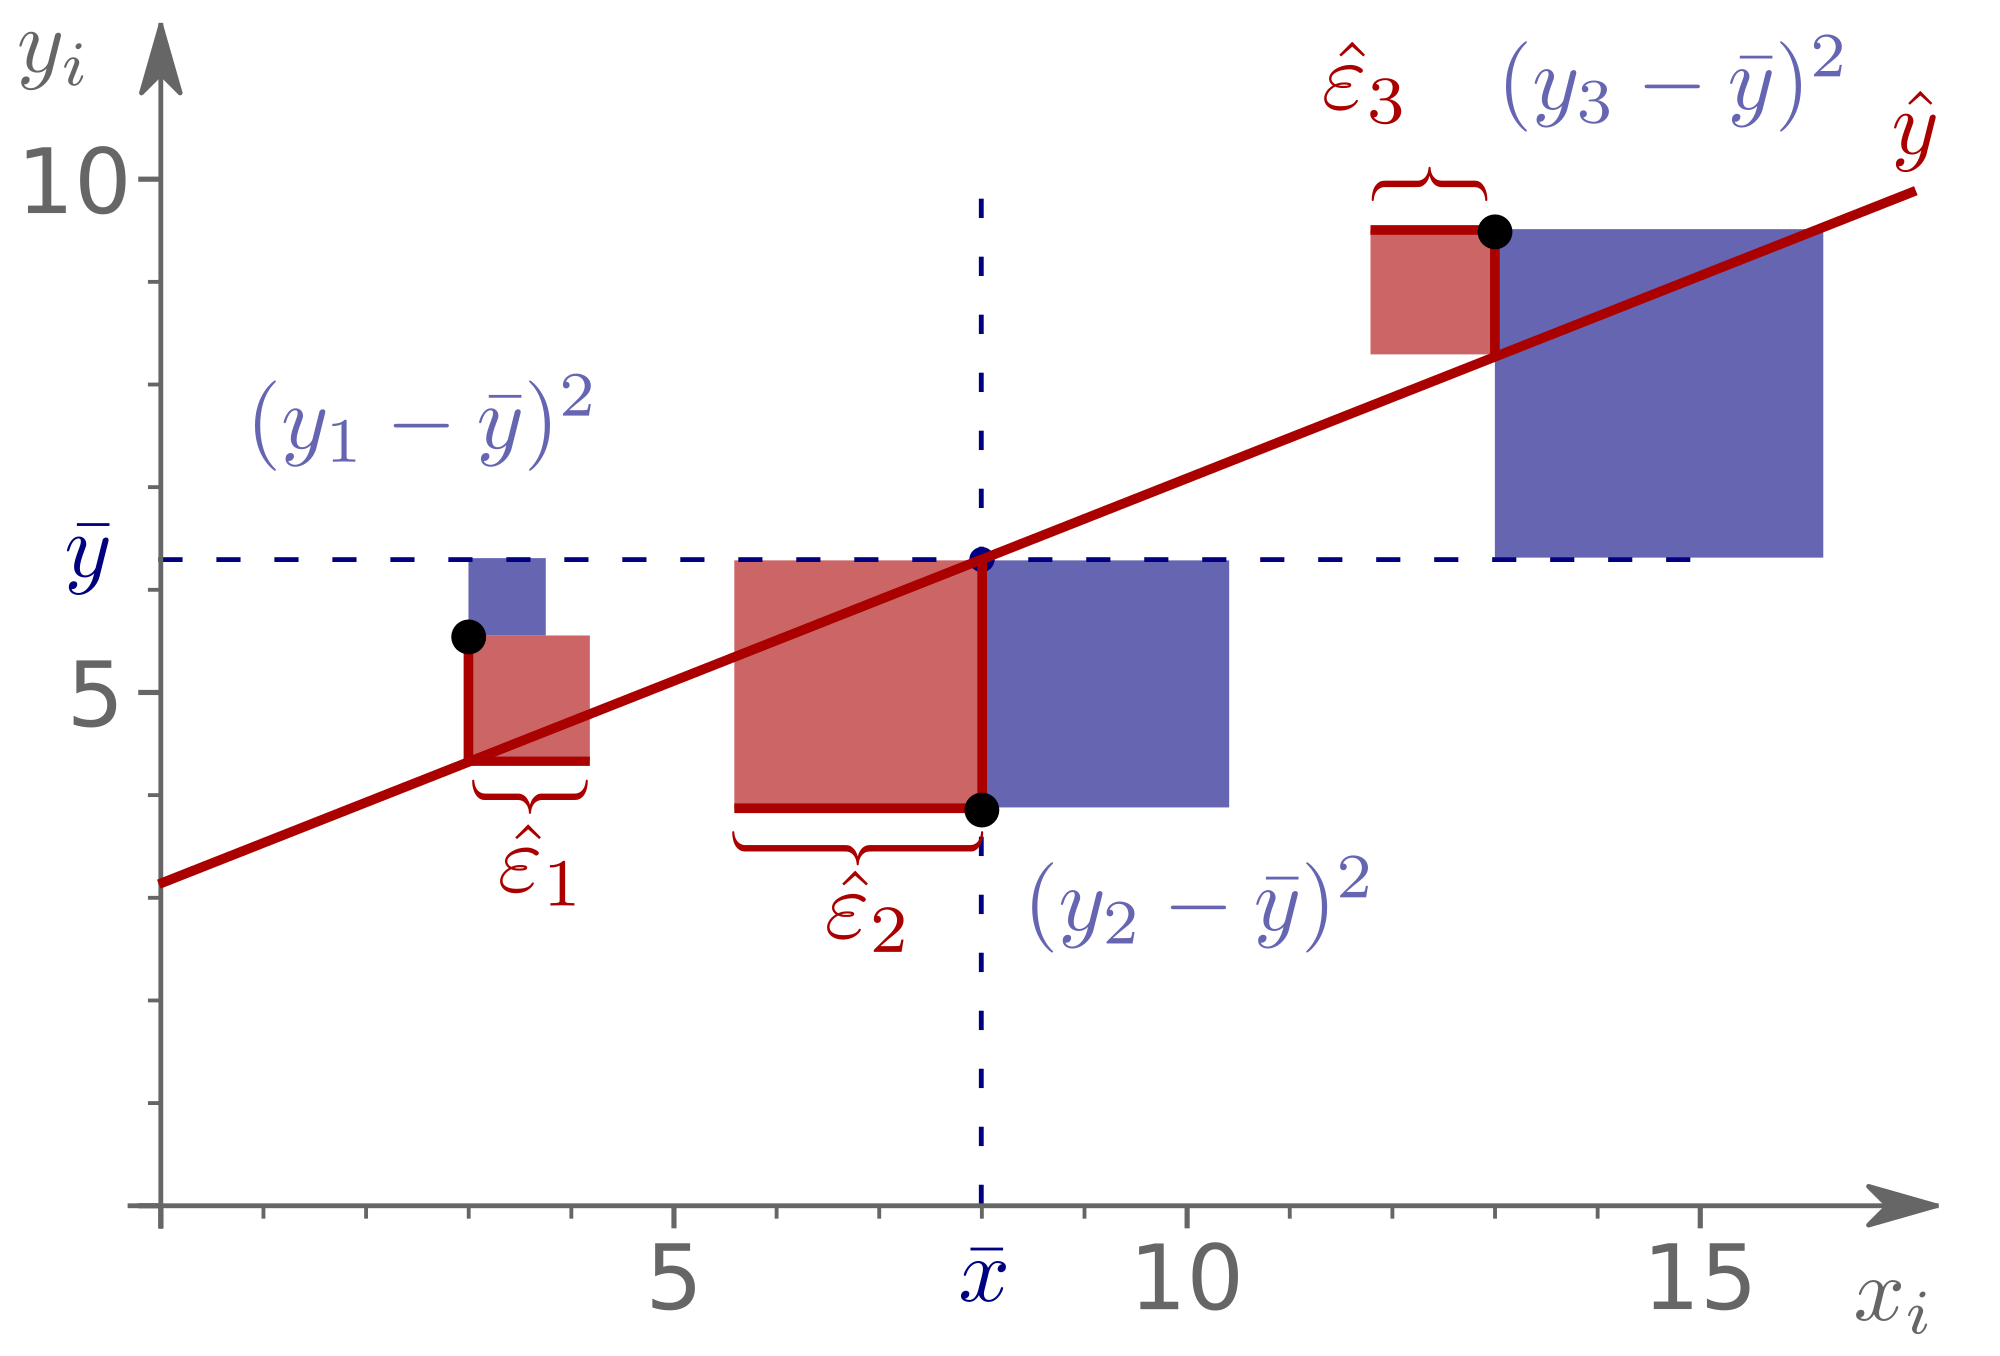
\includegraphics[width=\textwidth]{P17ols.png}	
			\credits{By Debenben at Wikipedia Commons. CC BY-SA 4.0.}											
		\end{fig}	
		The \emph{method of least squares}, also known as ordinary least squares (OLS), is one of the most common estimations used in linear regression. The method tries to draw the best fitting straight line into the datapoints $(x_n,y_n)$. By minimizing sum of the square of the distance between the line and each datapoint (the error or residuum), we will get the \emph{BLUE}, the best linear unbiased estimator.
		\begin{equation*}
			\min_{\beta_0,...,\beta_{k-1}} \sum\limits_{i=1}^n \left(y_i-\hat{y_i}\right)^2
		\end{equation*}
		This means, seeing this as a function $f(\beta_0,\beta_1,...\beta_{k-1})$ stating the sum of the squares of the differences between observed and estimated values, we are trying to minimize this function. With $\beta_0$ as a constant intercept, we can define $x_0\equiv 1$.
		\begin{equation*}
		\min_{\beta_0,...,\beta_{k-1}} f(\beta_0,\beta_1,...\beta_{k-1}) = \min_{\beta_0,...,\beta_{k-1}} \sum\limits_{i=1}^n \left(y_i-\hat{y_i}\right)^2 = \min_{\beta_0,...,\beta_{k-1}}  \sum\limits_{i=1}^n \left(y_i-\sum\limits_{j=0}^{k-1}\beta_j x_{ji} \right)^2
		\end{equation*}
		To find estimates of  $\beta_0,\beta_1,...\beta_{k-1}$ we find the derivative:
		\begin{equation*}
			\frac{\partial f(\cdot)}{\partial \beta_j}\quad\text{for }j\varepsilon\{0,1,...,k-1\}
		\end{equation*}
		\begin{align*}
				\frac{\partial f(\cdot)}{\partial \beta_0}&=\sum\limits_{i=1}^n -2\left(y_i-\sum\limits_{j=0}^{k-1}\beta_j x_{ji}\right)\qquad\text{(1)}\\
				&\vdots\\
				\frac{\partial f(\cdot)}{\partial \beta_j}&=\sum\limits_{i=1}^n -2\left(y_i-\sum\limits_{j=0}^{k-1}\beta_j x_{ji}\right)\qquad\text{(j)}\\				
		\end{align*}
		This means, $k$ equations for $k$ unknown $\beta$, so we can solve this. In matrix notation with $X$ as the matrix of explanatory observations, the solution will be (according to the method shown in appendix \ref{app:der}):
		\begin{equation*}
			\hat{\beta}=(X'X)^{-1}X'Y
		\end{equation*}
		From equation (1), we have
		\begin{equation*}
			 \sum\limits_{i=1}^n y_i-\sum\limits_{j=0}^{k-1}\beta_j   \sum\limits_{i=1}^n x_{ji}=0.
		\end{equation*}
		Dividing by $n$ gives us
		\begin{equation*}
			\underbrace{\frac{1}{n}\sum\limits_{i=1}^n y_{i}}_{=\bar{y}}-\sum\limits_{j=0}^{k-1}\beta_j \underbrace{\frac{1}{n}\sum\limits_{i=1}^n x_{ji}}_{=\bar{x}}=0
		\end{equation*}	
		\begin{equation*}
			\Longrightarrow \bar{y}=\sum\limits_{j=0}^{k-1}\hat{\beta_j}\bar{x_j}.
		\end{equation*}
		In other words, the regression line goes through the sample mean.
\subsubsection{Maximum Likelihood}
	The idea of this method is to \emph{maximize the likelihood} or chance of getting our sample when observing a population. This means to puck a parametric family and find the parameters that maximize the chance of observing the sample. Recall, assumptions A1-A6 (\ref{sec:ass}): $y_i\sim N\left((x)_i\beta,\sigma^2\right)$. Let $f(\cdot)$ designate the joint distribution of $\{y_1,y_2,...,y_n\}$.
	
	But we assumed that the error terms $\epsilon$ (and therefore $y_1,y_2,...,y_n$) are from a random sample and thus i.i.d. In consequence, the joint density of $y_1,y_2,...,y_n$ is equal to the products of the marginal densities of $y_1,y_2,...,y_n$.
	\begin{exmp}[Density of a normal distribution]{exmp:normdens}
		$W$ is normally distributed: $W\sim N(\mu,\sigma^2)$. Then, the density of $W$ is:
		\begin{equation*}
			f(w)=\frac{1}{\sqrt{2\pi\sigma^2}}\,exp\left[-\frac{1}{2}\left(\frac{w-\mu}{\sigma}\right)^2\right]
		\end{equation*}
	\end{exmp}
	In consequence, the joint density of $y_1,y_2,...,y_n$ is:
	\begin{equation*}
		f(y,x,\beta,\sigma^2)=\prod_{i=1}^{n}\frac{1}{\sqrt{2\pi\sigma^2}}\,exp\left[-\frac{1}{2}\left(\frac{y_i-\sum\limits_{j=0}^{k-1}\beta_j x_{ij}}{\sigma}\right)^2\right]
	\end{equation*}
	$f(\cdot)$ is a product of small values (all factors in the product are $\leq 1$). This makes exact calculations hard. Also, taking the derivative for maximizing the function is less convenient with a product function than with a sum. So before maximizing the function, we perform a logarithmic transformation. The log-likelihood function then is as follows:
	\begin{align*}
		\mathcal{L}(\beta,\sigma^2|y,x)&=ln\left(\prod_{i=1}^{n}\frac{1}{\sqrt{2\pi\sigma^2}}\,exp\left[-\frac{1}{2}\left(\frac{y_i-\sum\limits_{j=0}^{k-1}\beta_j x_{ij}}{\sigma}\right)^2\right]\right)\\
		&=-\frac{n}{2}ln(2\pi)-\frac{n}{2}ln(\sigma^2)-\frac{1}{2\sigma^2}\sum\limits_{i=1}^n\left(y_i-\sum\limits_{j=0}^{k-1}\beta_j x_{ij}\right)^2\\
		\frac{\partial\mathcal{L}}{\partial\sigma^2}&=0-\frac{n}{2}\frac{1}{\sigma^2}+\frac{1}{2\sigma^4}\sum\limits^n_{i=1}\left(y_i-\sum\limits_{j=0}^{k-1}\beta_j x_{ij}\right)^2\\
		\Longrightarrow \hat{\sigma}^2&=\frac{1}{n}\sum\limits_{i=1}^n(			\underbrace{y_i-\hat{y_i}}_{=\hat{\epsilon_i}})^2\\
		&=\frac{1}{n}\sum\limits_{i=1}^n \hat{\epsilon_i}=\frac{1}{n}\sum\limits_{i=1}^n \left(\hat{\epsilon_i}-E(\hat{\epsilon_i})\right)^2
	\end{align*}
	With $E(\hat{\epsilon_i})=0$. This expression is similar to calculating the variance as seen in definition \ref{defi:variance}. In this sense, we can see it as the variance of the error. Let us write $\mathcal{L}$ as follows:
	\begin{align*}
		\mathcal{L}&=-\frac{n}{2}ln(2\pi)-\frac{n}{2}ln(\sigma^2)-\frac{1}{2\sigma^2}\underbrace{(Y-X\beta)'}_{\hbox{row}}\underbrace{(Y-X\beta)}_{\hbox{column}}\\
		&=-\frac{n}{2}ln(2\pi)-\frac{n}{2}ln(\sigma^2)-\frac{1}{2\sigma^2}\sum\limits_{i=1}^n \left(y_i - \sum\limits_{j=0}^{k-1} \beta_j x_{ij} \right)^2\\
		\frac{\partial\mathcal{L}}{\partial\sigma^2}&=\frac{1}{n}\sum\limits_{i=1}^n \hat{\epsilon}_i,\qquad\text{Recall: }E(\epsilon_i)=0\\
		\frac{\partial\mathcal{L}}{\partial\beta}&=0+0-\frac{1}{2\sigma^2}\frac{\partial}{\partial\beta}\left[y'y-y'x\beta-\beta'x'y+\beta\right]\\
		&=-\frac{1}{2\sigma^2}\left[0-2x'y+2x'x\beta\right]\\
		\text{Recall: }G(\beta)&=\beta' M \beta,\quad \frac{\partial G}{\partial\beta}=M'\beta+M\beta\\
		(x'x)'&=x'x''=x'x\\
		\text{With symmetry }M&=M'\\
		M'\beta+M\beta&=2M\beta\\
		\frac{\partial\mathcal{L}}{\partial\beta}&=0\Longrightarrow\left[x'y=(x'x)\beta\right]\\
		\Longrightarrow\hat{\beta}&=(x'x)^{-1}x'y\\
		\text{Provided }rank(x'x)&=k\quad (x'x \text{ has an inverse})
	\end{align*}
\subsubsection{Properties of OLS \& ML estimators}
	\myparagraph{Expected value}
		\begin{align*}
			E(\hat{\beta})&=E\left((x'x)^{-1}x'y\right)=(x'x)^{-1}x'E(y)\\ %%x'xx is known and non-random (A5),y is N(x \beta, \sigma^2 I)
			%from a2: y=x\beta+\epsilon = x\beta
			\text{With }x\text{ as a known an non-random variable}
			E(\hat{\beta})&=(x'x)^{-1}x'x\beta=\beta\\
			E(\hat{\beta})&=\beta
		\end{align*}
		This means, $\hat{\beta}$ is an unbiased estimator.
	\myparagraph{Variance}
		\begin{align*}
			\hat{\beta}&=(x'x)^{-1}x'y=(x'x)^{-1}x'(X\beta+\epsilon)\\
			&=(x'x)^{-1}x'x\beta+(x'x)^{-1}x'\epsilon\\
			&=\beta+(x'x)^{-1}x'\epsilon\\
			\text{Recall: Let W be a random variance. Then: }\\
			var(W)&=E\left((W-E(W))^2\right)\\
			var(\hat{\beta})&=E\left((\hat{\beta}-\beta)(\hat{\beta}-\beta)'\right)\\
			&=E\left((x'x)^{-1}x'\epsilon\epsilon'x(x'x)^{-1}\right)\\
			&=(x'x)^{-1}x'E(\epsilon\epsilon')x(x'x)^{-1}\\
			&=(x'x)^{-1}x'\sigma^2 I_n x(x'x)^{-1}\\
			&=\sigma^2 (x'x)^{-1}x'x(x'x)^-1=\sigma^2(x'x)^{-1},\,(x'x)^{-1}x'x=I_k\\
			var(\hat{\beta})&=\sigma^2(x'x)^{-1}\\
			\widehat{var(\hat{\beta})}&=\hat{\sigma^2}(x'x)^{-1}\\
			\hat{\beta}&=\begin{pmatrix}
				\hat{\beta}_0\\
				\hat{\beta}_1\\
				\vdots\\
				\hat{\beta}_{k-1}
			\end{pmatrix}
		\end{align*}
		The standard error is the square root of the variance.
		\begin{gather*}
			SE(\hat{\beta}_j)=\sqrt{\hat{\sigma^2}(x'x)^{-1}_{jj}}\\
			var(\hat{\beta})=\begin{pmatrix}
				var(\hat{\beta}_0)&cov(\hat{\beta}_0,\hat{\beta}_1)&\cdots&cov(\hat{\beta}_0,\hat{\beta}_{k-1})\\
				cov(\hat{\beta}_1,\hat{\beta}_0)&var(\hat{\beta}_1)&\cdots&cov(\hat{\beta}_1,\hat{\beta}_{k-1})\\
				\vdots&\vdots&\ddots&\vdots\\
				cov(\hat{\beta}_{k-1},\hat{\beta}_0)&cov(\hat{\beta}_{k-1},\hat{\beta}_1)&\cdots&var(\hat{\beta}_{k-1})
			\end{pmatrix}
		\end{gather*}
	\myparagraph{Gauss-Markov theorem}
		Assume that A1-A5 (\ref{sec:ass1}) hold. Then, the ML-OLS estimators achieve minimum variance in the class of linear, unbiased estimators. So, they are most efficient.
		
		\emph{Proof:} Let $\tilde{\beta}$ be another linear, unbiased estimator. Without loss of generality, we write
		\begin{align*}
			\tilde{\beta}&=\hat{\beta}+Dy=\left[(x'x)^{-1}+D\right]y\\
			E(\tilde{\beta})&=\beta\quad(\tilde{\beta}\text{ is unbiased })\\
			E(\tilde{\beta})&=E\left(\left[(x'x)^{-1}x'+D\right]\left[x\beta+\epsilon\right]\right)\\
			&=\underbrace{(x'x)^{-1}x'x}_{I_k}\beta+Dx\beta+\left[(x'x)^{-1}x'+D\right]\underbrace{E(\epsilon)}_{=0\,(A2)}\\
			&=\beta+Dx\beta=(I+Dx)\beta=\beta\Longrightarrow Dx=0\\
			var(\tilde{\beta})&=var(Cy)=C var(y)C'=C\sigma^2 I_m C'\\
			&=\sigma^2 C C'\\
			&=\sigma^2 \left[(x'x)^{-1}x'+D\right]\left[(x'x)^{-1}x'+D'\right]\\
			&=\sigma^2 \left[(x'x)^{-1}\underbrace{x'x(x'x)^{-1}}_{I_k}+\underbrace{(x'x)^{-1}x'D'}_{=0}+D D' +\underbrace{Dx(x'x)^{-1}}_{=0}\right]\\
			&=\sigma^2(x'x)^{-1}+\sigma^2 D D'\\
			&=var(\hat{\beta})+\sigma^2 D D'
		\end{align*}
		$D D'$ is positive semi-definite, i.e. $\forall v,\,v' D D' v=(D'v)'(D'v)\geq 0$. Recall, this means that $norm(D'v)\geq 0$.	So, $var(\tilde{\beta})$ is larger than the variance $var(\hat{\beta})$. As a consequence, $\hat{\beta}$ is BLUE (\ref{sec:ols}). Linearity here means, in $y,\,\hat{\beta}=(x'x)^{-1}xy)$ with $x$ known.\begin{famo}[Carl Friedrich Gauß]{famo:gauss}
			\emph{Johann Carl Friedrich Gauß} (30 April 1777 – 23 February 1855) in Brunswick, in the Duchy of Brunswick-Wolfenbüttel (now part of Lower Saxony, Germany, as the son of poor working-class parents. \emph{Gauß was a child prodigy}. A contested story relates that, when he was eight, he figured out how to add up all the numbers from 1 to 100. 

Gauß' intellectual abilities attracted the attention of the Duke of Brunswick, who sent him to the Collegium Carolinum (1792 to 1795, and to the University of Göttingen (1795 to 1798). While there, Gauß independently rediscovered several important theorems. In 1796, he became the first to prove the quadratic reciprocity law, which allows mathematicians to \emph{determine the solvability of any quadratic equation}. He also conjectured the prime number theorem, which gives a good understanding of how prime numbers are distributed among integers. In his 1799 doctorate, Gauß proved \emph{that every nonconstant single-variable polynomial with complex coefficients has at least one complex root}.  Gauß also made important contributions to number theory in his 1801 book Disquisitiones Arithmeticae.

In 1831 Gauß developed a fruitful collaboration with physicist Wilhelm Weber, leading to new knowledge in magnetism and the \emph{discovery of Kirchhoff's electric circuit laws}. They constructed the first electromechanical telegraph in 1833, which connected the observatory with the institute for physics in Göttingen. In 1840, Gauß published his influential \enquote{Dioptrische Untersuchungen}, in which he gave the first systematic analysis on the formation of images under a paraxial approximation (\emph{Gaußian optics}).

Gauß' personal life was overshadowed by the early death of his first wife, Johanna Osthoff, in 1809, soon followed by the death of one child, which caused him to become depressed. When his second wife died in 1831 after a long illness, one of his daughters took over the household and cared for Gauß for the rest of his life. Gauß had six children, 3 with each wife. 
 
Gauß made major contributions to various areas of mathematics (including geometry and number theory) and physics (including magnetism and optics). The importance of his contributions is often compared to those of Newton. He also made some key contributions to statistics. The most important one is the development of \emph{least squares estimation recursive methods}, which he discusses in a book on planetary orbits. He also proposed some, which are used for time series analysis and were used to help calculate the trajectory of the Apollo spacecraft. He is also \emph{credited with developing the normal distribution} (also called the Gaussian distribution or bell curve), which is extremely useful in probability and statistics.
\credits{Sources: \url{https://en.wikipedia.org/wiki/Carl_Gauss}, \url{http://www.sciencedirect.com/science/article/pii/0315086078900496}}
		\end{famo}	
			
\subsubsection{Inference}
	Let us now also assume that A6 (\ref{sec:ass6}, normality of $\epsilon$) holds. Since $\hat{\beta}$ is a linear estimator (in $y$), and since $y\sim N(x\beta,\sigma^2 I_n)$ with i.i.d., then $\hat{\beta}$ as a linear combination of a independent normals is also normal distributed.
	\myparagraph{Hypothesis Testing}
		From the fact that $\hat{\beta}\sim N$,
		\begin{equation*}
			z^*=\frac{\hat{\beta}_l-\beta_{l0}}{\sigma(\hat{\beta}_l)}\sim N(0,1)
		\end{equation*}
		with $l\varepsilon\{0,1,...,k-1\}$, $\sigma(\hat{\beta}_l)$ as the standard error of $\hat{\beta}$ which is the square root of its variance. 
		
		In practice, we do not know $\sigma(\hat{\beta}_l)$. Because of that, we use
		\begin{equation*}
			T^*=\frac{\hat{\beta}_l-\beta_{l0}}{s(\hat{\beta}_l)}\text{. If $H_0$ is true, } t*\sim t(n-k)\text{ with } k=\#\text{ of }\beta\text{ in the model.}
		\end{equation*}
	\myparagraph{Confidence Interval}
			We have, given $\alpha\varepsilon(0,1)$,
			\begin{equation*}
				CI(1-\alpha)=\hat{\beta}_l\pm t_{\frac{\alpha}{2}}(n-k)\cdot s(\hat{\beta}_l)
			\end{equation*}
		\myparagraph{Joint test (f-test)}
			\emph{Step 1:}
			\begin{align*}
				H_0:\; &\beta_l=0\,\wedge\,\beta_{l+1}=0\,\wedge\,\cdots\wedge\,\beta_{k-1}=0\\
				H_1:\; &\text{not }H_0
			\end{align*}
			
			\emph{Step 2:}
			\begin{equation*}
				F^*=\frac{(SSE_R-SSE_F)/\#restrictions}{SSE_F/(n-k)}
			\end{equation*}
			with $\#restrictions=k-l$.
			If $H_0$ is true, $F^*\sim F(k-l,n-k)$.
			$SSE$ is the sum of the square errors $SSE=\sum\limits_{i=1}^n\hat{\epsilon_i^2}$.
			$R$ are parameters for the restricted model (obtained by imposing $H_0$) and $F$ of the full model with $k= \#$ of $\beta$.
			
			\begin{exmp}[Restricted linear model]{exmp:restr}
				$y_i=$ demand for bikesharing at location $i$.
				\begin{align*}
					F:\; y_i&=\beta_0+\beta_1 Inc_i +\beta_2 GenZ_i+\beta_3 GenY_i+\beta_4 GenX_i+\beta_5 Edu_i+\beta_6 Carpp_i +\epsilon_i\\
					R:\; y_i&=\beta_0+\beta_1 Inc_i +\beta_2 GenZ_i+\beta_3 GenY_i +\mu_i						
				\end{align*}
				Joint test: $H_0: \beta_4=0\,\wedge\,\beta_5=0\,\wedge\,\beta_6=0$					
			\end{exmp}
			
			\emph{Step 3:}
				\begin{enumerate}[	a.]
					\item Pick $\alpha=Pr(\text{Type I error})$,
					\item calculate $F^*_{calc}$,
					\item rejection region and locate $F^*_{calc}$, and
					\item conclude.
				\end{enumerate}
				\begin{exmp}[Testing for different values than zero]{exmp:othertests}
					Compare to the test for parameters to be zero in example \ref{exmp:restr}.
					\begin{align*}
						y_i&=\beta_0+\cdots+(1+\beta_6)Carpp_i+\epsilon_i\\
						R:\; y_i&=\beta_0+\cdots+\beta_3 GenY_i+Carpp_i+\mu_i
					\end{align*}
					Joint test: $H_0: \beta_4=0\,\wedge\,\beta_5=0\,\wedge\,\beta_6=0$
				\end{exmp}				
	\subsubsection{Goodness of Fit}
		\myparagraph{Square Errors}
			$R^2$ is the fraction of the variation of the dependent variable explained by the model. Consider $\{y_1,y_2,...,y_n\}$ as our dependent variable. One way to measure the variations of $y$ is
			\begin{equation*}
				SST=\sum\limits_{i=1}^n(y_i-\bar{y})^2
			\end{equation*}
			with $SST$ as the total sum of squares. One way to characterize how much a linear model \emph{explains} the variations of $y$ is:
			\begin{equation*}
				SSR=\sum\limits_{i=1}^n(\hat{y_i}-\bar{y})^2
			\end{equation*}
			\begin{equation*}
				R^2\equiv\frac{SSR}{SST}
			\end{equation*}
			We also can define
			\begin{equation*}
				SSE=\sum\limits_{i=1}^n \hat{\epsilon}^2_i
			\end{equation*}
			with $SSE$ as the square sum of errors and $SST=SSR+SSE$.
			\begin{align*}
				SST&=\sum\limits_{i=1}^n (y_i-\bar{y})^2=\sum\limits_{i=1}^n (y_i\hat{y}_i+\hat{y}_i-\bar{y})^2\\
				&=\sum\limits_{i=1}^n (y_i-\hat{y}_i)+2\sum\limits_{i=1}^n (y_i-\hat{y})(\hat{y}_i-\bar{y})+\sum\limits_{i=1}^n (\hat{y}_i-\bar{y})^2\\
				\sum\limits_{i=1}^n \hat{\epsilon}_i(\hat{y}_i-\bar{y})^2&=\hat{\epsilon}'\cdot(x\hat{\beta}-\bar{y}1)=\hat{\epsilon}' x\cdot \hat{\beta}-\bar{y}\hat{\epsilon}'1\\
				\hat{\epsilon}'x&=(y-\hat{y})'x=(y-x(x'x)^{-1}x'y)'x\\
				&=(y'-y'x(x'x)^{-1}x')x\\
				&=y'(x-x(x'x)^{-1}x'x)=y'(x-x)=0\\
				\hat{\epsilon}'1&=\sum\limits_{i=1}^n=\hat{\epsilon}_i=0
			\end{align*}
			because $E(\epsilon)=0$ which comes from $\frac{\partial \mathcal{L}}{\partial\beta_0}=0$.
			In consequence,
			\begin{align*}
				SST&=SSR+SSE\\
				R^2&=\frac{SSR}{SST}\\
				SSR,SST,SSE&\geq 1\\
				\Longrightarrow 0\leq R^2 &\leq 1
			\end{align*}
			Limitation of $R^2$ is that it will increase with the numbers of explanatory variables. It reflects the benefits of adding more variables, but not the cost of including them: the precision with which the $\beta$ are certain, their standard error. As a result, statisticians have introduced
			\begin{equation*}
				\bar{R^2}=1-\frac{SSE/(n-k)}{SSR(n-1)}=1-\frac{n-1}{n-k}\frac{SSE}{SST}=1-\frac{n-1}{n-k}(1-R^2)
			\end{equation*} 
			because
			\begin{equation*}
				\frac{SSE}{SST}=\frac{SSE+SSR-SSR}{SST}=\frac{SST-SSR}{SST}=1-\frac{SSR}{SST}=1-R^2.
			\end{equation*}
			We still have that $\bar{R^2} \leq 1$ but now $\bar{R^2}$ can be $\leq 0$. Higher values of $R^2$, close to 1, indicate a better fit.
		\myparagraph{Model F-test}
			\begin{equation*}
			y_i=\beta_0+\beta_1 x_{i1}+\beta_2 x_{i2}+\cdots+\beta_{k-1} x_{i\,k-1}+\epsilon_i
			\end{equation*}				
			Most statistical softwares perform \emph{model F-tests} by default. They test:
			\begin{equation*}
				H_0:\;\beta_1=0\,\wedge\,\beta_1=0\,\wedge\,\cdots\,\wedge\,\beta_{k-1}=0\quad H_1:\; not\,H_0
			\end{equation*}
			If $H_0$ is true, $F^*\sim F(k-1,n-k)$.
							
			This means, $H_1$ is at least one $\beta\neq 0$. This F-test tells us about the usefulness of the model as whole.
			\begin{equation*}
				F^*=\frac{(SSE_R-SSE_F)/(k-1)}{SSE_F/(n-k)}
			\end{equation*}
			In general, necessarily $SSE_R\geq SSE_F$ because the explanatory variables of the restricted model are in the full model as well. Let us relate $F^*$ to $R^2$.
			\begin{equation*}
				F^*=\frac{\frac{SSE_R-SSE_F}{SST}/(k-1)}{\frac{SSE_F}{SST}/(n-k)}=\frac{\left(1-R^2_R-(1-R^2_F)\right)/(k-1)}{(1-R^2_F)/(n-k)}=\frac{(R^2_F-R^2_R)/(k-1)}{(1-R_F^2)/(n-k)}
			\end{equation*}
			What is $R^2_R$?
			\begin{align*}
				SSR_R&=\sum\limits_{i=1}^n (\hat{y}_i-\bar{y})^2\\
				\text{here: }&=\sum\limits_{i=1}^n (\bar{y}-\bar{y})^2\\
				R^2_R&=0\\
				\Rightarrow F^*&= \frac{R^2_F / (k-1)}{(1-R^2_F)/(n-k)}
			\end{align*}
		\myparagraph{Information criteria}
			There are measures of relative fit of a model that take parsimony into account. They provide a trade-off between complexity and simplicity.
			\begin{enumerate}
				\item Akaike Information Criterion (AIC)
					\begin{equation*}
						AIC=-2 ln(\mathcal{L}^*)+2k
					\end{equation*}
					with $ln(\mathcal{L}^*)$ as the value of log-likelihood function at $\hat{\beta}$ and $k$ as the number of $\beta$. Smaller AIC values indicate a better model because unnecessary complexity results in a higher AIC. A significant difference in the quality of models usually results in a AIC difference greater than 3.
				\item Bayesian Information Criterion (BIC)
					Also known as \textit{Schwarz information criterion}, the BIC is similar to AIC, but favors more parsimonious models because sample size is taken into account.
					\begin{equation*}
						BIC=-2 ln(\mathcal{L}^*)+k\,ln(n)
					\end{equation*} 
			\end{enumerate}
			We only can compare models estimated on the same dataset, but one does not need to be a subset of the other.
	\subsubsection*{Interpretation}
		\begin{exmp}[Gas mileage of a car]{exmp:gasmileage}
			\begin{equation*}
				mpg_i = \beta_0 + \beta_1 EngSze_i + \beta_2 Weight_i + \beta_3 cw + \beta_4 MY16+ \beta_5 MY17 + \beta_6 MY18 + \beta_7 MY19
			\end{equation*}
			Where $EngSze, Weight, DragCoeff$ are continuous and $MY16,MY17,MY18,MY19$ are categorical and therefore binary variables: $=1$ if yes, $=0$ otherwise.
		\end{exmp}
		Multicollinearity: when one explanatory $x_1$ variable is almost a linear correlation of the other explanatory variables $x_2,...x_{k-1}$:
		\begin{equation*}
			x_1=\alpha_0+\alpha_2 x_2 + \cdot \alpha_{k-1} x_{k-1} +\mu \longrightarrow R^2
		\end{equation*}
		Then we can calculate the \emph{Variance Inflation Factor}:
		\begin{equation*}
			VIF_1=\frac{1}{1-R^2_1}
		\end{equation*}
		If $VIF\geq 10$, the choice of variables should be improved.
\subsection{Verification of assumptions}
	It is essential to check the assumptions (\ref{sec:ass}) we made when we built our linear model.
	\myparagraph{Linearity}
		Before estimating our model, plot $y$ vs each continuous variable . If the relationship is \emph{far} from being linear, transform the explanatory variable (ln, power,...). Afterwards, plot $\hat{\epsilon}$ versus $\hat{y}$. There should be no trends, so the graph should be random distributed after the transformation.
	\myparagraph{Unbiasedness}
		$E(\epsilon)=0$. No need to check this assumptions, it is ensured by the estimation.
	\myparagraph{Homoscedasticity}
		We can detect heteroscedasticity (the opposite) if we have patterns when plotting $\hat{\epsilon}$ versus $\hat{y}$, they should be randomly distributed. Besides the graphical evaluation, it can be assessed with statistical tests such as \emph{Park}, \emph{Goldfield-Quandt} or \emph{White}. The model can also be estimated with robust standard errors so it can handle moderate deviations from homoscedasticity. If there is heteroscedasticity, it is not per se an issue for the model, but it becomes a problem for testing $\beta$.
	\myparagraph{Uncorrelated errors}
		This assumption is typically violated for time series or spatial data.
		\begin{exmp}[Time series]{exmp:timeseries}
			Consider $\begin{cases}
				y_k=\beta_0+\beta_1 x_t +\epsilon_t\\
				\epsilon_t=\rho \epsilon_{t-1} + \mu_t
			\end{cases}$
			with $\mu_t \sim N(0,\sigma^2_\mu)$ as an i.i.d. and $|\rho|<1$.
			
			We have:
			\begin{align*}
				\epsilon_t&=\rho \epsilon_{t-1} + \mu_t\\
				\epsilon_{t-1}&=\rho \epsilon_{t-2} + \mu_{t-1}\\
				\vdots\\
				\epsilon_{t-n+1}&=\rho \epsilon_{t-n} + \mu_{t-n+1}					
			\end{align*}
			By substitution:
			\begin{align*}
				\epsilon_t&=\mu_t + \rho \mu_{t-1} + \cdots + \rho^{n+1}\epsilon_{t-n+1}\\
				\epsilon_t&=\mu_t + \rho \mu_{t-1}+\cdots\\
				var(\epsilon_t)&=\sigma^2+\rho^2 \sigma^2 + \rho^2 \sigma^2 + \cdots 
				&= \sigma^2 (1+\rho^2 + \rho^4 + \rho^6 + \cdots)\\
				&=\frac{\sigma^2}{1-\rho^2}
			\end{align*}
			We know for $X$ as a random variable:
			\begin{align*}
				var(X)&=\sigma^2,\;E(X)=\mu\\
				a>0,\;var(aX)&=E\left((ax-E(aX))^2\right)\\
				&=E\left((ax-E(aX))^2\right)\\
				&=a^2 E\left(E(X-E(X))^2\right)\\
				&=a^2\sigma^2
			\end{align*}
			Suppose it holds for $n-1$:
			\begin{align*}
				&-\alpha\overbrace{(1+\alpha+\cdots+\alpha^{n-1})}^{=S}\\
				&=(1-\alpha)S=1-\alpha^n\\
				S&=\frac{1-\alpha^n}{1-\alpha}
			\end{align*}
			Here, $\rho^2=\alpha$ since $|\rho |<1$.
			\begin{equation*}
				\lim\limits_{n\rightarrow + \infty} S_n=\frac{1}{1-\alpha}
			\end{equation*}
		\end{exmp}				
		Example \ref{exmp:timeseries} tells us that under serial conditions, the errors are \textit{off} so OLS (or ML) is no longer efficient (but still unbiased and consistent). To detect a serial correlation, we can use the \emph{Durbin-Watson statistic} (DW)
		\begin{equation*}
			d=\frac{\sum\limits_{t=2}^T (\hat{\epsilon}_t - \hat{\epsilon}_{t-1})^2}{\sum\limits_{t=1}^T \hat{\epsilon}_t^2}
		\end{equation*}
		with $T$ as the number of observations. It can be shown that $d\approxeq 2(1-p)$ where $p$ is the sample autocorrelation of errors. Moreover, $0\leq d \leq 4$:
		\begin{equation*}\text{If }
			\begin{cases}
				d \ll 2\text{, then we have positive serial correlation.}\\
				d \gg 2\text{, then we have negative serial correlation.}				
			\end{cases}
		\end{equation*}
		The difficulty is that the distribution of $d$ depends on the explanatory variables within the model, so the DW test is not always conclusive. To test for $t$ positive series correlation at level $\alpha$ which is the probability of a type I error:
		\begin{equation*}\text{If }
			\begin{cases}
			d < d_{L,\alpha}\text{, then reject $H_0$ of no series correlation}\\
			d > d_{U,\alpha}\text{, then fail to reject }H_0\\		
			d_{L,\alpha}\leq d \leq d_{U,\alpha}\text{, then cannot conlcude}
			\end{cases}
		\end{equation*}
		With $d_{L,\alpha}$ as the lower and $d_{U,\alpha}$ as the upper bound. Similar for testing negative serial correlation:
		\begin{equation*}\text{If }
			\begin{cases}
			(4-d) < d_{L,\alpha}\text{, then reject $H_0$ of no series correlation}\\
			(4-d) > d_{U,\alpha}\text{, then fail to reject }H_0\\		
			d_{L,\alpha}\leq (4-d) \leq d_{U,\alpha}\text{, then cannot conlcude}
			\end{cases}
		\end{equation*}
		In transportation, we often analyze data with spatial correlation. If we ignore spatial correlation, our estimators may be biased and inconsistent.	
		%book refrence: Spatial Econometrics
	\myparagraph{Exogeneity of regressors}
		When some explanatory variables are not exogenous, so determined outside of the model, the ML or OLS estimators are no longer consistent. Some reasons for this inconsistency are:
		\begin{enumerate}
			\item Omitted variable is substantially correlated with the model's explanatory variable.
			\item $y$ and one of the explanatory variable are jointly determined.
				\begin{equation*}
					\begin{cases}
					y_i=\beta_0+\beta_1 x_i + \epsilon_i\\
					x_i=\gamma_0+\gamma_1 y_i + \gamma_2 \zeta_i + \mu_i
					\end{cases}
				\end{equation*}
			\item Some variables are measured with substantial errors, so systematically and large.
			\item The relationship between the dependent variable and the regressors is changing over time (non-stationarity).
		\end{enumerate} 
	\myparagraph{Normality of errors}
		All $\beta$ are still unbiased and consistent but the testing will be off. There are some methods to detect non-normality of errors:
		\begin{enumerate}
			\item Draw a histogram of $\hat{\epsilon}=y-\hat{y}$. It should be the bell-shaped \emph{Gaussian curve}.
			\item Generate a Q–Q (quantile-quantile) plot. The Q-Q plot shows the quantiles of $\hat{\epsilon}$ versus the quantiles of a $N(0,1)$. The plot should be a straight line.
			\item Formal tests of normality, e.g. the \emph{Lilliefors test} for small samples ($n\leq 2000$) or \emph{Jarque-Bera} for samples of $n\geq 2000$.
		\end{enumerate}
		\begin{exmp}[Jarque-Bera test]{exmp:jbtest}
			\begin{equation*}
				JB^*=\frac{n}{6}\left(g^2+\frac{(k-3)^2}{4}\right)
			\end{equation*}
			With $n$ as the size, $g$ as the skewness, and $k$ as the kurtosis of the sample. Under $H_0,\;JB^*\sim \chi^2(2)$.
		\end{exmp}
\subsection{Regression diagnostics}
 \subsubsection{Unusual and influential observations}
		The idea is, that if a single (or a few) observations are different from the rest of the sample they can have a big impact on the $\beta$. The goal is to detect these observations and to analyze them.
		
		An \emph{outlier} is an observation with a large estimated error $|\hat{\epsilon}|$. An observation is \emph{influential} if removing it substantially changes one or more $\beta$. How to detect outliers?
		\begin{itemize}
			\item Graph $\hat{\epsilon}_i$ versus $y_i$
			\item Generate and examine studentized residuals
		\end{itemize}
		The studentized residuals for observation $i$ is $\frac{\hat{\epsilon}_i}{\hat{\sigma}\sqrt{1-h_{ii}}}$ where $h_{ii}$ is $H_{ii}$ with $\underbrace{H}_{n \times n}=x(x'x)^{-1}x'$. $H$ is a symmetric matrix:
		\begin{align*}
			H'&=x''(x'x)^{-1}x'=x(x'x)^{-1}x'=H\\
			H^2&=x(x'x)^{-1}\underbrace{x'x(x'x)^{-1}}_{=I_k}x'=H
		\end{align*}
		Because $H^i=H\;\forall\;i$, $H$ is idempotent.
		
		Experience shows that we need to examine observations for which $|\hat{\epsilon}|\geq 2$. Influential means the observation has \emph{leverage}, thus we look for measures of leverage.
		\begin{itemize}
			\item One measure of leverage is $h_{ii}$.\\
				Rule of thumb: if $|h_{ii}|>\frac{2k}{n}$ with $k$ number of observations and sample size $n$, examine observation $i$.
			\item Another common measure of leverage is the \emph{Cook's distance}.\\
				\begin{equation*}
					D_i=\frac{\hat{\epsilon}^2_i}{k\cdot MSE}\left[\frac{h_{ii}}{(1-h_{ii})^2}\right]\geq 0
				\end{equation*}
				Rule of thumb: if $D_i \geq \frac{4}{n}$, examine observation $i$.
			\item Another measure of influence:
				\begin{equation*}
					dffits_i=\frac{\hat{y}_i-\hat{y}_{i-(i)}}{\hat{\sigma}_{(i)}\sqrt{h_{ii}}}
				\end{equation*}
				with $\hat{y}_{(i)}$ as the estimated $y_i$ after removing observation $i$ and $\hat{\sigma}_{(i)}$ as the the standard deviation of $\epsilon$ after removing observation $i$.

				Rule of thumb: if $|dffits_i|\geq 2 \sqrt{\frac{k}{n}}$, examine observation $i$.
			\item Alternatively, we can examine how observation $i$ impact $\beta_j$ using
				\begin{equation*}
					dfbeta_{j,i}\equiv \frac{\hat{\beta}_j-\hat{\beta}_{j(i)}}{\hat{\sigma}_{(i)}\sqrt{(x'x)^{-1}_{jj}}}
				\end{equation*}
				with $i=1,...,n$ and $j=0,1,...,k-1$.
				Rule of thumb: if $|dfbeta_{j,i}|\geq \frac{2}{\sqrt{n}}$, examine observation $i$. A limitation of this measure is that we should look at $(k-1)\times n\;dfbeta$ which grows to a large amount of measure values.	Also, if we have more than one influential observation and they are clustered the estimate will not work well.	
		\end{itemize}
	\subsubsection{Multicollinearity}
		We have \emph{multicollinearity} if one explanatory variables can be approximated by a linear combination of other explanatory variables. Without loss of generality, we can then say i.e.
		\begin{equation*}
			x_i \approxeq \alpha_0 + \alpha_2 x_2 + \cdots \alpha_{k-1} x_{k-1}
		\end{equation*}
		In case the approximate is exact, there is perfect collinearity which means $(x'x)^{-1}$ would not exist. This often happens if you forgot to exclude a categorical variable as a baseline (for $k$ categories we need to have exact $k-1$ binary, categorical, \enquote{dummy} variables). If the relationship is only approximate, you have a numerical problem: $(x'x)^{-1}$ is not calculated precisely and the standard errors of $\beta$ are going to be inflated, it will look like the $\beta$ are not statistically different from 0.
		
		To detect multicollinearity, calculate \emph{before} estimating your model $VIF_j=\frac{1}{1-R^2_j}$ where $R_j^2$ is the \enquote{$R^2$} from regressing $x_j$ on the other explanatory variables.
		
		Rule of thumb: $\begin{cases}
		\text{if }VIF_j\geq 10\text{, there is a clear multicollinearity problem.}\\
		\text{if }5\leq VIF_j\leq 10\text{, there could be multicollinearity problem (gray area).}\\	
		\text{if }VIF_j\leq 5\text{, there is no multicollinearity problem.}\\						
		\end{cases}$
		
		Remedies:
		\begin{enumerate}
			\item If the problem is mild ($MAX VIF\varepsilon[5,10]$), do nothing but document the problem.
			\item If the problem is more severe, drop some $x_j$.
			\item Collect more data for the model.
			\item \emph{Mean center \& standardize} explanatory variables: $x_j\rightarrow \zeta_j=\frac{x_j-\bar{x_j}}{s_j}$.
			\item Use specialized estimators (e.g. ridge regression instead of OLS).
		\end{enumerate}
		With the Cook's Distance and knowing $MSE=\hat{\sigma}^2$:
		\begin{equation*}
			D_i=\frac{\hat{\epsilon}^2_i}{k \hat{\sigma}^2}\left[\frac{h_{ii}}{(1-h_{ii})^2}\right]
		\end{equation*}		
		Use percentiles of $F(k,n-k)$. Find the percentile corresponding to $D_i$.
		$$\begin{cases}
			\text{If this percentile is }\leq 20\%\,i\text{ is not influential.}\\
			\text{If this percentile is }\geq 50\%\,i\text{ is influential.}\\
		\end{cases}$$
		In between, we cannot make a statement.
\subsection{Box-Cox transformation}
	The \emph{Box-Cox transformation} (B-C) can change non-normally distributed data to more normally distributed data. It applies to data which is $>0$ because it is a power transformation. It can be used both for continuous explanatory and dependent variables or only for some of those.
	\begin{align*}
		y_i&=\beta_0+\sum\limits_{j=1}^{k-i} \beta_j x_{ij}+\epsilon_i\\
		\longrightarrow\, y_i^\lambda &=\tilde{\beta}_0+\sum\limits_{j=1}^{k-i} \tilde{\beta}_j x_{ij}^\theta+\epsilon_i
	\end{align*}
	But only in case $x_{ij}$ is continuous, otherwise leave the variable unchanged.
	$$\begin{cases}
		\text{If } \lambda=0 \text{, replace }y_i^\lambda \text{ with } ln(y_i)\\
		\text{If } \theta=0 \text{, replace }x_{ij}^\theta \text{ with } ln(x_{ij})\\
	\end{cases}$$
	\begin{defi}[Box-Cox transformation]{defi:boxcox}
		$$x_{ij}^*=\begin{cases}
			\frac{x_{ij}^\theta -1}{\theta}\text{ if }\theta\neq 0\\
			ln(x_{ij})\text{ if }\theta= 0\\
		\end{cases}$$
		$\lambda$ and $\theta$ can be obtained by maximum likelihood, so the product of marginal likelihoods for observing our sample is maximized.			
	\end{defi}
	See also the density of a normal distribution as shown in example \ref{exmp:normdens}.	
	$$\mathcal{L}(\beta,\sigma^2,\lambda,\theta|y,x)=\prod_{i=1}^{n} \frac{1}{\sqrt{2\pi\sigma^2}}exp\left[-\frac{1}{2}\left(\frac{y_i^\lambda-(\beta_0+\beta_1 x_{i1}^\theta+\cdots+\beta_{k-1} x_{ik-1}^\theta)}{\sigma}\right)^2\right]$$		
	\begin{exmp}[Continuity of Box-Cox]{exmp:boxcoxcont}
		Let $x>0$:
		\begin{gather*}
			\lim\limits_{\theta\rightarrow 0} \frac{x^\theta -1}{\theta} \approxeq \frac{1+\theta ln(x) -1}{\theta}=ln(x)\\
			x^\theta= e^{\theta ln(x)}
		\end{gather*}
		If $\theta$ is small, $e^{\theta ln(x)}\approxeq 1+\theta ln(x)$.
		With the expansion:
		\begin{gather*}
			e^\epsilon \approxeq 1+\epsilon\\
			e^\epsilon=\sum\limits_{n=0}^{+\infty} \frac{\epsilon^n}{n!}
		\end{gather*}
	\end{exmp}
\subsection{Tobit models}
	 We frequently encounter datasets where observations are clustered at the lower and/or at the upper bound. This could result for example from observations going beyond what is measured or correspond to a different behavior. We cannot ignore this feature and simply estimate a linear regression model because in this case its estimator would be biased and inconsistent. One solution to deal with this problem is the \emph{Tobit model}, named after James Tobin (1958).
	\begin{defi}[Tobit model]{defi:tobit}
		The version where the clustering of values is at lower bound 0:
		\begin{equation*}
			y_i=\begin{cases}
				y_i^* \text{ if }y_i^* \geq 0\\
				0 \text{ otherwise}\\
			\end{cases}
		\end{equation*}
		where
		\begin{equation*}
			y_i^*=\beta_0+\sum\limits_{j=1}^{k-1} \beta_j x_{ij} + u_i,\; u_i \overset{i.i.d.}{\sim}N(\sigma,\sigma^2).
		\end{equation*}
	\end{defi}
	$y_i^*$ is a latent variable that is observable (unobserved) only when $y_i \geq 0$. Model parameters can be obtained by maximum likelihood.
	\begin{equation*}
		\mathcal{L}=\prod_{i=1}^{n}\left[\frac{1}{\sigma}\varphi\left(\frac{y_i-x_i \beta}{\sigma}\right)\right]^{d_i} \left[1\Phi\left(\frac{x_i \beta}{\sigma}\right)\right]^{1-d_i} %Pr(y^* \leq 0) letzter faktor %todo
	\end{equation*}
	where
	\begin{align*}
		\varphi&\equiv\text{ the density of a standard normal distribution }\\
		\Phi&\equiv\text{ the cumulative for a standard normal distribution }\\
		\sigma&\equiv\text{ the standard deviation of } u_i\\
		d_i&=\begin{cases}
			1\text{ if } y_i>0\\
			0\text{ otherwise}
		\end{cases}	
	\end{align*}
	For this model,
	\begin{align*}
		E(Y)&=Pr(Y^* \geq 0)\cdot E\left[Y|Y\geq 0\right]+ Pr(Y^* < 0)\cdot E\left[Y|Y< 0\right]\\%todo uppercase is random var
		E(Y)&=\Phi\left(\frac{x_i \beta}{\sigma}\right)\left[x_i \beta + \sigma \frac{\varphi \left(\frac{x_i \beta}{\sigma}\right)}{\Phi \left(\frac{x_i \beta}{\sigma}\right)}\right]
	\end{align*}
	where $\frac{\varphi \left(\frac{x_i \beta}{\sigma}\right)}{\Phi \left(\frac{x_i \beta}{\sigma}\right)}$ is named \emph{Mill's ratio}. 
	
	This model can be generalized to lower bounds different from 0, upper boundaries, and both.
	\begin{equation*}
		y_i=\begin{cases}
			y_i^* \text{ if }y_L \leq y_i^* \leq y_U\\
			y_L \text{ if }y_i^* < y_L\\
			y_U \text{ if }y_i^* < y_U\\
		\end{cases}
	\end{equation*}
	For more details see \textcite{Wooldridge.2016}.
\section{Models for Discrete Dependent Variables}
%%%%%%%%%%%%%%%%%%%%%%%%%%%%%%%%
In transportation, there are many cases where the dependent variable of interest is \emph{not continuous}.

Examples:
\begin{enumerate}
	\item Binary: $\begin{cases}
			1 \text{ if you travel to a national park this weekend}\\
			0 \text{ otherwise}
		\end{cases}$
	\item Categorical: mode choice to LAX $\begin{cases}
			\text{ rideshare}\\
			\text{ train}\\
			\text{ shuttle}\\
			\text{ car}
		\end{cases}$
	\item Ranked data
	\item Count data
\end{enumerate}
\subsection{Models for binary outcomes}
	Typically, the values are 0 or 1.  The models shown here are non-linear. They explain the probability of observing either 0 or 1 as an outcome.
	\subsubsection{Statistical model}
		Three ways to introduce these models:
		\begin{enumerate}
			\item Latent variable
			\item Random utility
			\item Probability model
		\end{enumerate}
		\myparagraph{Latent variable approach}
			The latent variable approach (with latent in the meaning of \textit{unobserved}) gives us the probability to observe one outcome for the dependent variable $y$.. Let $y$ be a (0,1) binary variable. Let $x_1,x_2,...,x_{k-1}$ be independent variables we consider using to explain $y$. The key idea is to assume there exists a latent continuous variable $y^*$ which is related to the $x$ as follows:
			\begin{align*}
				y^*_i&=x_i \beta + \epsilon_i\\
				y_i&=\begin{cases}
					1\text{ if } y_i^*>0\\
					0\text{ otherwise}
				\end{cases}
			\end{align*}
			$y^*_i$ can be interpreted as the potential that the event of interest will occur. From our model we know
			\begin{align*}
				Pr(y_i=1|x_i)&=Pr(y_i^*>0|x_i)\\
				&=Pr(x_i \beta > 0 | x_i)=Pr(-\epsilon_i<x_i \beta | x_i)
				&=F(x_i \beta) \longrightarrow
			\end{align*}
			with $F(\cdot)$ as a cumulative distribution statement. Depending on the distributional assumption for $\epsilon_i$, we get different models.
			\begin{itemize}
				\item If $\epsilon_i  \overset{i.i.d.}{\sim}N(0,1)$, we obtain the binary probit model
					\begin{equation*}
						Pr(y_i=1|x_i)=\int\limits_{-\infty}^{x_i \beta} \frac{1}{\sqrt{2 \pi}} e^{-\frac{u^2}{2}} du
					\end{equation*}
				\item If $\epsilon_i  \overset{i.i.d.}{\sim}L(0,\frac{\pi^2}{3})$, we obtain the binary logit model
					\begin{equation*}
					Pr(y_i=1|x_i)=\frac{exp(x_i \beta)}{1+exp(x_i \beta)}
					\end{equation*}
					With $L(\cdot)$ as a logistic distribution. This term represents a \emph{proper} probability because it returns values in the interval $(0,1)$.
			\end{itemize}
			\begin{defi}[Odds function]{defi:oddsf}
				The \emph{odds function} is given by:
				\begin{equation*}
					\Omega(x_i)=\frac{Pr(y_i=1|x_i)}{Pr(y_i=0|x_i)}=\frac{Pr(y_i=1|x_i)}{1-Pr(y_i=1|x_i)}\quad \varepsilon(0,+\infty)
				\end{equation*}
				The odds function represents the ratio of the probability of the event happening (outcome 1) over the event not happening (outcome 0).
			\end{defi}
			For the logit model, the odds function becomes:
			\begin{align*}
				\Omega(x_i)&=\frac{\frac{exp(x_i \beta)}{1+exp(x_i \beta)}}{1-\frac{exp(x_i \beta)}{1+exp(x_i \beta)}}\\
				&=exp(x_i \beta)=e^{x_i \beta}\\
				\Rightarrow ln\left(\Omega(x_i)\right)&=x_i \beta		
			\end{align*}
	\subsubsection{Interpretation}\label{sec:binint}
		\myparagraph{Logit model}
			It is easier to interpret because we have an explicit expression for the model probabilities. As an example, consider the case with 3 explanatory variables:
			\begin{align*}
				\Omega(x_1,x_2,x_3)&=exp(x_0+\beta_1 x_1+\beta_2 x_2 + \beta_3 x_3)\\
				\Omega(x_1+1,x_2,x_3)&=exp(x_0+\beta_1 (x_1+1)+\beta_2 x_2 + \beta_3 x_3)\\
				&=exp(x_0+\beta_1 x_1+\beta_2 x_2 + \beta_3 x_3)\cdot exp(\beta_1)\\
				\Rightarrow exp(\beta_1)&=\frac{\Omega(x_1+1,x_2,x_3)}{\Omega(x_1,x_2,x_3)}
			\end{align*}
			So, for a unit change in $x_i$, the odds change by a factor $e^{\beta_i}$ holding all other variables constant. Note that with $p=Pr(y=1,x)$:
			\begin{align*}
				\Omega&=\frac{p}{1-p}\\
				\Rightarrow \Omega(1-p)&=p\\
				\Rightarrow \Omega&=p(1+\Omega)\\
				\Rightarrow p&=\frac{\Omega}{1+\Omega}			
			\end{align*}
			For the logit, another way to present results is to look at the percentage change in odds:
			\begin{equation*}
				\frac{\Omega(x_1+1,x_2,x_3)-\Omega(x_1,x_2,x_3)}{\Omega(x_1,x_2,x_3)}=(e^{\beta_1}-1)
			\end{equation*}
			\begin{exmp}[Probability of a event in a logit model]{exmp:problog}
				With the latent variable approach:
				\begin{align*}
					y_i&=\begin{cases}
						1 \text{ if } y_i^*\equiv x_i \beta + \epsilon_i \geq 0\\
						0 \text{ otherwise}\\
					\end{cases}\\
					\epsilon_i  &\overset{i.i.d.}{\sim}L(0,\frac{\pi^2}{3})\text{ logit model}\\
					\longrightarrow Pr(y_i=1|x_i)&=\frac{e^{x_i \beta}}{1+e^{x_i \beta}}
				\end{align*}
			\end{exmp}
		\myparagraph{More general interpretation}
			Plot predicted provabilities versus explanatory variables as seen in Figure \ref{fig:logit}. Fix the other explanatory variables and only plot the change over one $x_j$ (only works for the case of $x_j$ being continuous). In case $x_j$ is discrete, generate table of probabilities instead.
			\begin{fig}[Logistic model]{fig:logit}{h}
				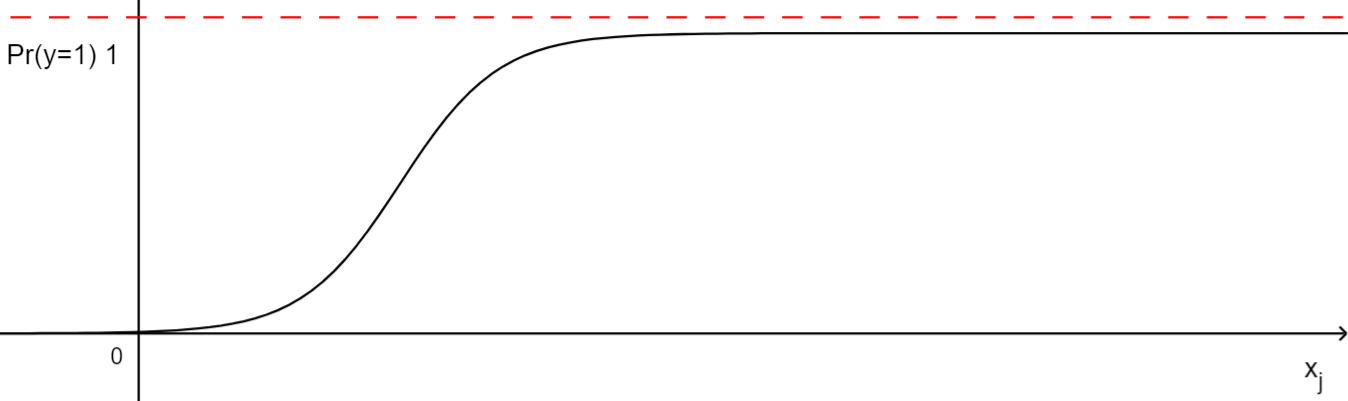
\includegraphics[width=\textwidth]{P18logit.png}	
			\end{fig}				
		\myparagraph{Marginal Changes}
			The third possibility is to report \emph{marginal changes} in probabilities across the sample
			\begin{equation*}
				\frac{\partial Pr(y_i=1|x_i)}{\partial x_{ij}}
			\end{equation*}
			with $x_{ij}$ as a continuous explanatory variable.
	\subsubsection{Measures of fit}\label{sec:mofit}
		A number of different measures of fit have been proposed.
		\begin{itemize}
			\item $Count\,R^2=\frac{\#\,of\,correct\,model\,predictions}{samplesize}$
			\item $McFadden's\,R^2:\,\rho^2=1-\frac{ln(\mathcal{L}^*_{full})}{ln(\mathcal{L}^*_{intercept})}$ where $\mathcal{L}^*_{intercept})$ is the model with no explanatory variables. A larger value indicates a better model.
			\item $McFadden's\,adjusted\,\hat{R}^2:\,\hat{\rho}^2=1-\frac{ln(\mathcal{L}^*_{full})-k}{ln(\mathcal{L}^*_{intercept})}$ with $k$ as the number of $\beta$ in the model (compare to $\bar{R}^2$ for linear regression).
		\end{itemize}
		 The idea of the measures is that if a model is not explaining much, $ln(\mathcal{L}^*_{full})$ is going to be close to $ln(\mathcal{L}^*_{intercept})$ and so McFadden's (adjusted) $R^2$ will be close to 0.
		 		
		 Model parameters are obtained by maximum likelihood. The likelihood function for a random sample is given by
		 \begin{align*}
		 	\mathcal{L}&=\prod_{i=1}^{n} Pr(y_i=1|x_i)^{y_i}\cdot (Pr(y_i=1|x_i))^{1-y_i}\\
		 	y_i&=\begin{cases}
			 	1\\0\\
		 	\end{cases}\\
		 	\text{For the logit: }Pr(y_i=1|x_i)&=\frac{e^{x_i \beta}}{1+e^{x_i \beta}}
		 \end{align*}
		 $\mathcal{L}$ is a product of probabilities $\mathcal{L} < 1$ so $ln(\mathcal{L})< 0$. Hence, $0>ln(\mathcal{L}^*_{full})>ln(\mathcal{L}^*_{intercept})$. In consequence,
		 \begin{equation*}
		 	\frac{ln(\mathcal{L}^*_{full})}{ln(\mathcal{L}^*_{intercept})}\leq 1\text{ so, }1-\frac{ln(\mathcal{L}^*_{full})}{ln(\mathcal{L}^*_{intercept})}\geq 0.
		 \end{equation*}
	\subsubsection{Hosmer-Lemeshow statistic}
		The \emph{Hosmer-Lemeshow statistic} is used to asses if the model is well-specified. The idea is to compare predicted probabilities with observed data. The steps are:
		\begin{enumerate}
			\item Fit the model.
			\item Compute predicted probabilities ($\hat{\pi}_i \equiv Pr(y_i=1|x_i)$).
			\item Sort the data by $\hat{\pi}_i$ from smallest to largest.
			\item Divide observations in $G$ groups ($G\approx 10$), so each group has $\approx \frac{10}{G}$ observations.
			\item Within each group, calculate the mean prediction $\bar{\pi}_g=\left(\sum\limits_{i\varepsilon g} \hat{\pi}_i \right) \frac{1}{n_g}$ with $n_g$ as the number of observations in group $g$.
			\begin{equation*}
				\bar{y}_g=\frac{1}{n_g} \sum\limits_{i\varepsilon g} y_i
			\end{equation*}
			\item Calculate the Hosmer-Lemeshow statistic $HL^*$:
			\begin{equation*}
				HL^*=\sum\limits^{G}_{g=1}\frac{(n_g \bar{y}_g - n_g \bar{\pi}_g)^2}{n_g \bar{\pi}_g (1-\bar{\pi}_g)}
			\end{equation*}
		\end{enumerate}
		If the model is well-specified, $HL^*\sim\chi^2(G-2)$. %todo threshold for decision if it is good or not
	\subsection{Models for nominal outcomes}
		An example for a nominal outcome is mode choice in transportation. This includes unordered variables with more than two outcomes.
		\subsubsection{General model}
			Models are described in more detail in \citetitle{Train.2009} by \textcite{Kennedy.2008}.
			
			Consider a decision maker who has different alternatives for a cause of action. We call this alternatives a \emph{choice set}. We assume that
			\begin{itemize}
				\item these alternatives are mutually exclusive,
				\item the choice set is exhaustive (it contains all alternatives of interest), and
				\item the number of alternatives (elements in the choice set) is finite.
			\end{itemize}
			In addition, it is assumed that the decision maker is going to pick the alternative that maximizes his utility, denoted by $U_{nj}$ where $n$ is an index for the decision maker and $j$ an index for the alternative.
			
			Hence, alternative $i$ is preferred if and only if $\forall\,j\varepsilon\{1,...,J\},\,U_{ni}\geq U_{nj}$ with $J$ number of alternatives.
			
			A researcher does not know the preferences of the decision makers. She observes some of their attributes (stored in vector $s_n$ for decision maker $n$) and some characteristics of each alternative (stored in vector $x_{nj}$). A function is specified that relates $s_n$ ad $x_{nj}$ to decision maker's $n$ utility:
			\begin{equation*}
				V_{nj}\equiv V(x_{nj},s_n)\text{ for }j\varepsilon\{1,...,J\},\,n\varepsilon\{1,...,N\}
			\end{equation*}
			The representative utility $V_{nj}$ is not equal to the actual utility $U_{nj}$ because of incomplete information, expressed by an error term:
			\begin{equation*}
				U_{nj}=V_{nj}+\epsilon_{nj}
			\end{equation*}
			Then, we can express the probability that person $n$ picks alternative $i$ as the probability its utility is higher:
			\begin{align*}
				P_{ni}&=Pr(U_{ni}\geq U_{nj},\forall j \varepsilon \{1,...,J\} )\\
				&=Pr(V_{ni}+\epsilon_{ni}\geq V_{nj}+\epsilon_{nj},\forall j \varepsilon \{1,...,J\} )\\
				&=Pr(\epsilon_{nj}-\epsilon_{ni}\leq V_{nj}-V_{ni},\forall j \varepsilon \{1,...,J\} )			
			\end{align*}
			This is a cumulative distribution statement. Depending on the choice of distribution for $\epsilon_{nj}$, we obtain a different model. In general, $P_{ni}$ is a $J-1$ dimensional integral (because it expresses a difference). Such integrals are usually computationally challenging, especially for cases with large $J>4$. The following assumptions simplify the calculation:
			\begin{equation}
				\epsilon_{nj} \overset{i.i.d.}{\sim} N(0,\sigma_{nj}^2)
			\end{equation}
			In that case:
			\begin{equation}
				\epsilon_{nj}-\epsilon_{ni} \sim N(0,\sigma_{nji}^2)
			\end{equation}
			Then,
			\begin{equation}
				\sigma^2_{nji}=var(\epsilon_{nj})-2cov(\epsilon_{nj}, \epsilon_{ni})+var(\epsilon_{ni})
			\end{equation}
			which leads to the multinomial probit model.
			
			Instead, we assume $\epsilon_{nj} \overset{i.i.d.}{\sim} EV(1)$, the Gumbel distribution.\\
			The CDF of a Gumbel $(\omega,\eta)$ is:
			\begin{equation*}
				F(\zeta)=e^{-e^{\eta(\zeta-\omega)}}
			\end{equation*}
			The corresponding PDF is:
			\begin{equation*}
				f(\zeta)=-\eta e^{-\eta(\zeta-\omega)} e^{-e^{\eta(\zeta-\omega)}}
			\end{equation*}
			Typically, we assume $\omega=0$ and $\eta=1$. For that assumptions, the variance of the Gumbel distribution becomes $\frac{\pi^2}{6}$. In that case, it can be shown that:
			\begin{equation*}
				P_{ni}=\frac{e^{+V_{ni}}}{\sum\limits^J_{j=1} e^{+V_{nj}}}
			\end{equation*}
			This result comes from the fact that the difference of two i.i.d. Gumbels is a logistic distribution. It is easy to check that $0<P_{ni}<1$ and $\sum\limits^J_{j=1} P_{ni}=1$.

			For convenience, $V_{nj}$ is assumed to be linear function of $s_n$ and $x_{nj}$:
			\begin{equation*}
				V_{nj}=\underbrace{y_{nj}}_{1xk} \underbrace{\beta_j}_{kx1}
			\end{equation*}
			
			Only the difference in utility is of matter. So, we can set the value of one alternative specific constant. The scale of utility is arbitrary, so we need to set the variance of the errors in our model.
		\subsubsection{Measures of fit}\label{sec:mofitMNL}
			The measures of fit are similar to the ones used for binary models (\ref{sec:mofit}). We need to know the expression of the likelihood function:
			\begin{align*}
				\mathcal{L}(\beta|y,x)&=\prod_{i=1}^{n} \prod_{j=1}^{J} P_{nj}^{\mathcal{G}(y_n=j)}\\
				\mathcal{G}(y_n=j)&=\begin{cases}
					1 \text{ if } y_n=j\\
					0 \text{ otherwise}
				\end{cases}
			\end{align*}
		\subsubsection{Interpretation}
			In general, we can use the same approaches as for binary models (\ref{sec:binint}).
			\myparagraph{Calculating predicted probabilities}
				\begin{equation*}
					P_{nm}=\hat{Pr}(y_n=m|x)=\frac{exp(x\hat{\beta}_{m|J})}{\sum\limits^J_{j=1}exp(x\hat{\beta}_{j|J})}
				\end{equation*}
				This equation is for the logit model with alternative $J$ as the baseline.
			\myparagraph{Special case of the multinomial logit model}
				\begin{equation*}
					Pr(y_i=m|x_i)=\frac{exp(x_i \beta_{m|J})}{\sum\limits^J_{j=1}exp(x_i \beta_{j|J})}
				\end{equation*}
				Let
				\begin{align*}
					\Omega_{m|J}(x_i)&=\frac{Pr(y_i=m|x_i)}{Pr(y_i=J|x_i)}\\
					&=x^{x_i \beta_{m|J}}
				\end{align*}
				Let $\Omega_{m|J}(x_i)$ be the odds that observations $i$ selects alternative $m$ given $J$ as the baseline. Let then $\Omega_{m|J}(x_i,x_{il}+1)$ be the odds obtained by adding 1 to the explanatory variable $l$. Then:
				\begin{equation*}
					\frac{\Omega_{m|J}(x_i,x_{il}+1)}{\Omega_{m|J}(x_i)}=e^{\beta_{m|J,l}}
				\end{equation*}
			\myparagraph{Back to the general case}	
				Select a \textit{profile}, so pick the explanatory variables to correspond to a \textit{typical decision-maker} with \textit{typical choices} and for continuous explanatory variables, plot the change of probability $P_{ni}$ over the explanatory variable $x_il$. For discrete explanatory variables, create a table to store the different values for probabilities for the $J$ alternatives when the discrete variables change by one unit.
				
				Also, the change in predicted probabilities can be calculated for predicted probabilities:
				\begin{equation*}
					\frac{\partial Pr(y_i=m|x_i)}{\partial x_{il}}
				\end{equation*}
		\subsubsection{Specification problems}\label{sec:specprob}	
			\myparagraph{Omitted variables}
				If a \textit{relevant} explanatory variable is omitted, multinomial parameter estimates are inconsistent if
				\begin{enumerate}
					\item the omitted variable is correlated with included explanatory variable, or
					\item the omitted variable is correlated across alternative outcomes or has a different variance for different outcomes.
				\end{enumerate} 
			\myparagraph{The errors are not i.i.d.}
				In this case, the parameter estimators will be inconsistent.
			\myparagraph{Parameters are not quite stationary}
				In this case, the parameter estimators will be inconsistent as well (similar to the issues when estimating a linear model for measures which alter over time instead of observations constant for the model).
			\myparagraph{Only for multinomial logit: Independence of irrelevant alternatives (IIA)}
				This is specific problems for multinomial logit models (MNL) and does not apply to other models.
				
				Recall that for $(m,n)\varepsilon\{1,...,J\}^2$:
				\begin{align*}
					Pr(y=m)&=\frac{e^{x\beta_{m|J}}}{\sum\limits^J_{j=1}e^{x\beta_{m|J}}}\\
					Pr(y=n)&=\frac{e^{x\beta_{n|J}}}{\sum\limits^J_{j=1}e^{x\beta_{n|J}}}\\					
					\frac{Pr(y=m)}{Pr(y=n)}&=\frac{e^{x\beta_{m|J}}}{e^{x\beta_{n|J}}}
				\end{align*}
				This ratio does \emph{not depend} on the characteristics of alternatives other than $m$ and $n$. Adding or deleting alternatives should not affect such ratios.
				
				This property (which applies only to MN logit models) is called \emph{independence of irrelevant alternatives (IIA)} and should be tested.
				
				For the test, estimated coefficients from a full model are compared to those of a restricted model (where restricted means that at least one alternative has been removed).
				
				There are two common tests:
				\begin{enumerate}
					\item \emph{Hausmann-McFadden (1984)}\\
					Step 1: Fit the full model with $J$ alternatives $\hat{\beta}_F$\\
					Step 2: Fit a restricted model by eliminating one or more alternatives $\hat{\beta}_R$\\
					Step 3: Let $\hat{\beta}^*_F$ be the subset of $\hat{\beta}_F$ corresponding to $\hat{\beta}_R$\\
					Step 4: Calculate test statistic $HM=(\hat{\beta}_R-\hat{\beta}_F^*)'\left[\widehat{var}(\hat{\beta}_R)-\widehat{var}(\hat{\beta}_F^*)\right]^{-1}(\hat{\beta}_R-\hat{\beta}_F^*)$. If IIA holds, $HM\sim \chi^2(dim(\hat{\beta}_R))$.			
					\item \emph{Small-Hsiao (1985)}\\
					The test randomizes the sample, so repeating the test will lead to different results.
				\end{enumerate}
				Neither of the tests is very reliable.
		\subsubsection{Extensions and testing of coefficients}
			\begin{itemize}
				\item One coeffcient: t-test
				\item x-cofficients: F-test or likelihood test
			\end{itemize}
			Same as before, a number of extensions have been proposed for models for nominal outcomes, built around the logistic distribution but do not require the IIA to hold, for example \emph{nested logit} or \emph{cross-nested logit} (see \textcite{Train.2009}).
	\subsection{Models for ordered outcomes}	
		In many transportation applications, we obtain ordered data. For example:
		\begin{enumerate}
			\item Quantitative ratings or rankings (scale 1 to 5)
			\item Ordered opinions or reviews
			\item Categorical frequency data (e.g. crash w/ fatalities, crash w/ injuries, w/o injuries)
		\end{enumerate}		
		If ordering of the is not taken into account (so it is taken as categorical), the estimator will lose efficiency. Linear regression would be inconsistent because the distance is not meaningful. However, just the fact that the values of a variable can be ordered \emph{does not imply that an ordinal model is appropriate}. For example, answering \enquote{don't know} does not equate \enquote{neutral}, which means the outcomes are not fully ordered.
		
		\subsubsection{Statistical model}
			We rely on a latent-variable approach (McKelvey \& Zavoina, 1975). Consider a dependent variable $y$ that can take $J$ different values $\{1,2,...,J\}$.
			
			The model is then
			\begin{align*}
				y_i&=m\varepsilon\{1,...,J\}\text{ if and only if }\tau_{m-1}\leq y_i^*<\tau_m\text{ (Measurement model)}\\
				\text{with }\tau_0&=-\infty\,\wedge\,\tau_J=+\infty\\
				\text{where }y^*_i&=x_i \beta+\epsilon_i,\,i\varepsilon\{1,...,n\}\text{ (Structural model)}
			\end{align*}
			with the sample size $n$ and $\tau$ as the $J-1$ cutpoints or thresholds to estimate.
			\begin{exmp}[Model for questionnaire results]{exmp:questionnaire}
				We are analyzing a question with 4 outcomes:
				\textit{Strongly disagree (SD), disagree (D), agree (A), strongly agree (SA)}
				\begin{align*}
					y_i&=\begin{cases}
						1=SD\text{ if }\tau_0\equiv -\infty \leq y_i^* < \tau_1\\
						2=D\text{ if }\tau_1 \leq y_i^* < \tau_2\\
						3=D\text{ if }\tau_2 \leq y_i^* < \tau_3\\
						4=D\text{ if }\tau_3 \leq y_i^* < \tau_4\\
					\end{cases}\\
					y_i^*&=x_i \beta + \epsilon_i
				\end{align*}
			\end{exmp}
			\begin{align*}
				Pr(y_i=m|x)&=Pr(\tau_{m-1}\leq y_i^* < \tau_m | x_i)\\
				&=Pr(\tau_{m-1}\leq x_i\beta+\epsilon_i < \tau_m | x_i)\\
				&=Pr(\tau_{m-1}- x_i\beta \leq \epsilon_i < \tau_m -x_i \beta| x_i)\\	
				&=F(\tau_m-x_i\beta)-F(\tau_{m-1}-x_i \beta)
			\end{align*}
			Where $F$ is the CDF of $\epsilon_i$. Depending on the choice for distribution we of $\epsilon_i$, we obtain a different model. 	
			%TODO picture, probit model March 6
			We can estimate $\beta$ and $\tau=(\tau_1,...\tau_{J-1})$ using maximum likelihood. The likelihood function is:
			\begin{align*}
				\mathcal{L}(\beta,\tau|y,x)&=\prod_{i=1}^{n} \prod_{j=1}^{J} \left[F(\tau_j -x_i \beta)-F(T_{j-1}-x_i \beta)\right]^{\delta_{ij}}\\
				\text{where }\delta_{ij}&=\begin{cases}
					1\text{ if }y_i=1\\
					0\text{ otherwise}\\
				\end{cases}
			\end{align*}
			As usual, we need to take the log before maximizing this expression.
			
			For the ordered logit model, we have:
			\begin{equation*}
				Pr(y=m|x_i)=\frac{e^{\tau_m - x_i \beta}}{1+e^{\tau_m - x_i \beta}}-\frac{e^{\tau_{m-1} - x_i \beta}}{1+e^{\tau_{m-1} - x_i \beta}}
			\end{equation*}
		\subsubsection{Interpretation}
			Because ordered models are not linear, their interpretation is more complex and requires more than only one approach.
			\myparagraph{Predict probabilities for different profiles}
				Calculate $\widehat{Pr}(y_i=j|x_i),\,j\varepsilon\{1,...,J\}$ for selected values of x.
			\myparagraph{Visualize predicted probabilities}	
				The predicted probabilities of continuous explanatory variables are graphed as a function.
				%TODO picture March 6
			\myparagraph{Create table of predicted probabilities}
				The predicted probabilities of binary explanatory variables are can be showed in tables.
			\myparagraph{Marginal change in probabilities}
				For continuous variables, you can calculate marginal changes
				\begin{equation*}
					\frac{\partial Pr(y_i=m|x_i)}{\partial x_{il}}
				\end{equation*}	
				where $m\varepsilon\{1,...,J\}$ and $x_{il}$ as the $l$-th explanatory variable (assumed to be continuous) for person $i$.
			\myparagraph{Odds ratio for ordered logit model (OLM)}
				\begin{align*}
					Pr(y_i=m|x_i)&=\frac{e^{\tau_m-x_i\beta}}{1+e^{\tau_m-x_i\beta}}-\frac{e^{\tau_{m-1}-x_i\beta}}{1+e^{\tau_{m-1}-x_i\beta}}\\
					Pr(y_i\leq m|x_i)&=\frac{e^{\tau_m-x_i\beta}}{1+e^{\tau_m-x_i\beta}}-\frac{e^{\tau_{m-1}-x_i\beta}}{1+e^{\tau_{m-1}-x_i\beta}}\\
					&+\frac{e^{\tau_{m-1}-x_i\beta}}{1+e^{\tau_{m-1}-x_i\beta}}-\frac{e^{\tau_{m-2}-x_i\beta}}{1+e^{\tau_{m-2}-x_i\beta}}\\
					\vdots\\
					&+\frac{e^{\tau_{1}-x_i\beta}}{1+e^{\tau_{1}-x_i\beta}}-\frac{e^{\tau_{0}-x_i\beta}}{1+e^{\tau_{0}-x_i\beta}}\\
					\Longrightarrow Pr(y_i\leq m|x_i)&=	Pr(y_i= m|x_i)+Pr(y_i= m-1|x_i)+\cdots+Pr(y_i=1|x_i)\\
					\Longrightarrow Pr(y_i\leq m|x_i)&=\frac{e^{\tau_m-x_i\beta}}{1+e^{\tau_m-x_i\beta}}\\
					Pr(y_i> m|x_i)&=1-\frac{e^{\tau_m-x_i\beta}}{1+e^{\tau_m-x_i\beta}}=\frac{1}{1+e^{\tau_m-x_i\beta}}\\
					\frac{Pr(y_i\leq m|x_i)}{Pr(y_i> m|x_i)}&=e^{\tau_m-x_i\beta}\equiv \Omega_{\leq m / > m}(x_i)\\
					\frac{\Omega_{\leq m / > m}(x_i,x_{il}+1)}{\Omega_{\leq m / > m}(x_i)}&=\frac{e^{\tau_m-\left(\beta_l x_{i1}+\cdots\beta_1 (x_{il}+1) \right)+\cdots+\beta_k x_{ik}}}{e^{\tau_m-\left(\beta_l x_{i1}+\cdots\beta_1 x_{il} \right)+\cdots+\beta_k x_{ik}}}=e^{-\beta_l}
				\end{align*}	
				This states that for a unit increase in $x_{il}$, the odds that an outcome is $\leq m \varepsilon\{1,..,J\}$ change by a factor $e^{-\beta_l}$ holding all other variables constant.
		\subsubsection{Measures of fit}\label{sec:mofitOrd}
			The measures of fit for models with ordered outcomes are similar to the measures of fit for binary and multinominal logit models (\ref{sec:mofit} and \ref{sec:mofitMNL}).
			\begin{itemize}
				\item $Count\,R^2$ as the ratio of the number of correctly predicted outcomes by the number of observed units.
				\item $'s\,R^2$
				\item $McFadden's\,adjusted\,R^2$
			\end{itemize}			
		\subsubsection{Hypothesis testing}
			\myparagraph{Individual coefficients}
				Three steps for hypothesis testing:%todo ref to chapter
				\begin{enumerate}
					\item 	$H_0:\;\beta_l=\beta_{l0}\; vs. \;H_1:\;<\,\neq,\,>$
					\item	Use $z^*=\frac{\hat{\beta}_l-\beta_{l0}}{\hat{\sigma}_{\hat{\beta}_l}}$\\%todo
							If the model is well specified, $z^*\sim N(0,1)$ (standard normal).
					\item	Conclude the results.
				\end{enumerate}
			\myparagraph{Multiple coefficients}
				%todo picture Mar11
		\subsubsection{Specification Problems}
			The problems of multinominal models (\ref{sec:specprob}) apply here as well, but for models with ordered outcomes there is one additional issue.
			\myparagraph{Parallel regression assumption}
				Recall that for $m\varepsilon\{1,...,J\}$:
				\begin{align*}
					Pr(y=m|x)&=F(\tau_m-x\beta)-F(\tau_{m-1}-x\beta)\\
					\tau_{0}=-\infty\;&\wedge\;\tau_{J}=+\infty
				\end{align*}
				As a result, $Pr(y\leq m|x)=F(\tau_m-x\beta)$. For example, in the case of $J=4$ we have the probabilities as shown in GRAPHIC %TODO figure march 13
				
				\begin{equation*}
					Pr(y\leq m|x)=F\left(\right.\tau_m \underbrace{x\beta}_{-\text{independent of }m\left. \right)}
				\end{equation*}
				We have the same $\beta$ for each probability. This allows models for ordered outcomes to be more efficient than normal, categorical models with different parameters $\beta$ for different categories, which are the more general form:
				\begin{equation*}
					Pr(y\leq m|x)=F(\tau_m-\underbrace{x\beta_m}_{\text{dependent of }m})
				\end{equation*}		
				It is however a good idea to test if the assumption is correct that the $\beta$ in the statements $Pr(y\leq m|x)=F(\tau_m-x\beta_m)$ are equal, so a joint test along the more general model to asses whether it can be simplified to a model for ordered outcomes. There are different test available for this, most common is the \textit{Brant test} (1990).%todo check other named tests for formatting / emph etc
				
				Usually, it worths checking this assumption if then a model for ordered data can be used. These are attractive for ordered data because they are much more concise than just categorical models (by factor $J$).
	\subsection{Models for count data}		
		Count data is very common in transportation, some example include
		\begin{itemize}
			\item the number of (\#) vehicles waiting at a toll plaza,
			\item \# of trucks waiting at a warehouse,
			\item \# of accidents on a given road segment during a given time period, or
			\item \# of cars owned by households in a census tract.
		\end{itemize}
		Linear regression is not appropriate for this kind of question. Instead, some common count models are used. As for other discrete data models, count data models predict the probability of observing different outcomes.
		
		\myparagraph{Poisson model}
			The \emph{Poisson model} is one of the most common discrete count models. It is named after French mathematician Siméon Denis Poisson (1781-1840).
			\subsubsection{Statistical model}
				Let $N_i$ be a random variable that generates count data. Then,
				\begin{equation*}
					Pr(N_i=n)=\frac{e^{-\lambda_i}\lambda_i^n}{n!}
				\end{equation*}
				with $\lambda_i=e^{x_i\beta}$ as the arrival rate and $n\varepsilon\mathbb{N}$.
				This relation comes from the exponential expansion.
				\begin{equation*}
					e^{-\lambda}=1+\frac{(-\lambda)^1}{1!}+\frac{(-\lambda)^2}{2!}+\cdots\Rightarrow e^x=\sum\limits_{n=0}^{+\infty} \frac{x^n}{n!}
				\end{equation*}%todo maybe as expmp
				Clearly, $Pr(N_i=n)\geq 0$. Let us show that $\sum\limits_{n=0}^{+\infty} Pr(N_i=n)=1$.
				\begin{align*}
					\sum\limits_{n=0}^{+\infty} Pr(N_i=n)&=	\sum\limits_{n=0}^{+\infty} e^{-\lambda_i} \frac{\lambda_i^n}{n!}=e^{-\lambda_i} \sum\limits_{n=0}^{+\infty} \frac{\lambda_i^n}{n!}\\
					&= e^{-\lambda_i} e^{+\lambda_i} = e^0 = 1
				\end{align*}
				So, $Pr(N_i=n)$ is a proper probability.
				%todo exmp m be discrete expected value pic mar 13
				\begin{align*}
					E(N)&=	\sum\limits_{n=0}^{+\infty} n Pr(N=n)=	\sum\limits_{n=0}^{+\infty} n \frac{e^{-\lambda}\lambda^n}{n!}=e^{-\lambda} \sum\limits_{n=1}^{+\infty} \frac{\lambda^n}{(n-1)!}\\
					&=e^{-\lambda} \sum\limits_{n=1}^{+\infty} \frac{\lambda\cdot\lambda^{n-1}}{(n-1)!}=\lambda e^{-\lambda} \sum\limits_{k=0}^{+\infty} \frac{\lambda^k}{(k)!}\text{ with }k=n-1\\
					&=\lambda e^{-\lambda} e^{+\lambda}=\lambda=E(N)
				\end{align*}
				Using the knowledge of $E(N)=\lambda$, the variance can be calculated.
				\begin{align*}
					var(N)&=\sum\limits_{n=0}^{+\infty} (n-\lambda)^2 e^{-\lambda} \frac{\lambda^n}{n!}\\
					&=\sum\limits_{n=0}^{+\infty} (n^2-2 n \lambda + \lambda^2) e^{-\lambda} \frac{\lambda^n}{n!}\\
					&=\underbrace{\sum\limits_{n=0}^{+\infty} n^2 e^{-\lambda} \frac{\lambda^n}{n!}}_{=S_1} - \underbrace{2 \sum\limits_{n=0}^{+\infty} e^{-\lambda} \frac{\lambda^n}{n!}}_{=S_2}+ \underbrace{\lambda ^2 \sum\limits_{n=0}^{+\infty} e^{-\lambda} \frac{\lambda^n}{n!}}_{=S_3}\\
					S_1&=\sum\limits_{n=0}^{+\infty} \left[\right. \underbrace{n(n-1)}_{\rightarrow S_1^a}+\underbrace{n}_{\rightarrow S_1^b} \left.\right] e^{-\lambda}\frac{\lambda^n}{n!}\\
					S_1^a&=\sum\limits_{n=1}^{+\infty} (n-1) e^{-\lambda} \frac{\lambda^n}{(n-1)!}=\sum\limits_{n=1}^{+\infty} e^{-\lambda} \lambda^2 \frac{\lambda^{n-2}}{(n-2)!}=e^{-\lambda} \lambda^2 \sum\limits_{n=2}^{+\infty} \frac{\lambda^{n-2}}{(n-2)!}\\
					&=\lambda^2 e^{-\lambda} \sum\limits_{k=0}^{+\infty} \frac{\lambda^k}{k!}=\lambda^2 e^{-\lambda} e^{+\lambda}=\lambda^2 \qquad \text{ with }k=n-2\\
					S_1^b&=\sum\limits_{n=1}^{+\infty} e^{-\lambda} \frac{\lambda \lambda^{n-1}}{(n-1)!}=\lambda\\
					S_2&=\lambda\lambda=\lambda^2 \\
					S_3&=e^{-\lambda} \sum\limits_{n=0}^{+\infty} \frac{\lambda^n}{n!}=1\\
					\Rightarrow var(N)&=S_1^a+S_1^b-S_2+S_3=\lambda^2+\lambda-2\lambda^2+\lambda^2=\lambda=E(N)
				\end{align*}
				The equality of variance and expected value is called equidispersion.
			\subsubsection{Estimation}
				The $\beta_0$ in $\lambda_i=e^{x_i\beta}$ with $x_i$ as a row vector and $\beta$ as a column vector can be estimated by maximum likelihood.
				\begin{equation*}
					\mathcal{L}(\beta|x)=\prod_{i=1}^{n} e^{-\lambda_i(\beta) \frac{\lambda_i^{n_i}(\beta)}{n_i!}}
				\end{equation*}
				with $n_i$ as the observed counts and 
				\begin{equation*}
					e^{-\lambda_i(\beta) \frac{\lambda_i^{n_i}(\beta)}{n_i!}}=Pr(N_i=n_i)
				\end{equation*}
				as the probability of $n_i$ to be observed. The log of this function is numerically easy to estimate. The Poisson ML estimation is consistent, asymptotically normal and asymptotically efficient.
			\subsubsection{Interpretation}
				Consider a discrete change $\delta$ in continuous variable $x_{il}$.
				\begin{align*}
					\frac{E\left(N_i|x_i,x_{il}+\delta \right)}{E\left(N_i|x_i\right)}&=\frac{e^{\beta_0+\beta_1 x_{1l}+\cdots+\beta_l (x_{il}+\delta) \cdots \beta_{k-1} x_{ik-1}}}{e^{\beta_0+\beta_1 x_{1l}+\cdots+\beta_l (x_{il}) \cdots \beta_{k-1} x_{ik-1}}}\\
					E\left(N_i|x\right)&=\lambda_i=e^{x_i\beta}
				\end{align*}
				So if $\delta=1$, we get $e^{\beta_l}$. This means, $\beta_l$ is the log of the ratio of expected counts when $x_l$ is increased by 1 unit.
				
				If $x_l$ is continuous, the elasticity of $\lambda_i$ with respect to $x_l$ is
				\begin{equation*}
					\frac{\partial \lambda_i}{\partial x_l} \frac{x_l}{\lambda_i}=\beta_l \lambda_i \frac{x_l}{\lambda_i}=\beta_l x_l,\;\lambda_i=e^{x_i\beta}.
				\end{equation*}
				
				The marginal change in $\lambda_i$ with respect to $x_l$ is
				\begin{equation*}
					\frac{\partial \lambda_i}{\partial x_l}=\beta_l \lambda_i.
				\end{equation*}				
			\subsection{Measures of fit}
			The measures of fit are similar to the methods of pseudo-squared deviance estimators used for other discrete models (\ref{sec:mofit}, \ref{sec:mofitMNL}, and \ref{sec:mofitOrd}).
				\begin{itemize}
					\item $McFadden's\,R^2:\,\rho^2=1-\frac{max\,logLikelihoodFullModel}{max\,logLikelihoodRestricteModel}=\frac{LL_f(\beta^*)}{LL_r(0)}$
					\item $McFadden's\,adjusted\,R^2$
					\item $Count\,R^2$		
				\end{itemize}			
			\subsection{Testing}
				%todo similar like before, see lr 2(ln)... resticition
				
				
			\myparagraph{Negative binomial regression model (NBR)}	
				In many cases, $E(N)\neq var(N)$. If  $E(N) > var(N)$, we name it underdispersion, in case  $E(N)< var(N)$	it is called overdispersion.
				
				One possibility to deal with this problem is to add an error term to the equation of $\lambda_i$.
				\begin{equation*}
					\lambda_i=e^{x_i\beta+\epsilon_i}
				\end{equation*}
				If $e^{\epsilon_i}\overset{i.i.d.}{\sim} \Gamma(1,\alpha)$, we obtain the NBR. For the NBR, $var(N_i)=E(N_i)+\alpha E^2(N_i)$.
				\begin{equation*}
					Pr(N_i=m)=\frac{\Gamma (n+\alpha^{-1})}{\Gamma (\alpha^{-1})n!}\left(\frac{\alpha^{-1}}{\alpha^{-1}+\lambda_i}\right)\left(\frac{\lambda_i}{\alpha^{-1}+\lambda_i}\right)^n
				\end{equation*}
				where
				\begin{align*}
					\Gamma(\zeta)&=\int_{0}^{+\infty} e^{-t} t^{\zeta-1} dt\\
					\Gamma(n)=(n-1)!
				\end{align*}

				The estimation of NBR models is similar to the Poisson models:
				\begin{equation*}
					\mathcal{L}=\prod_{i=1}^{n} Pr(N_i=n_i)
				\end{equation*}
				Also, the interpretation, measuring of fit and testing follow the same framework. An additional test for the equidispersion of $\alpha$ can be necessary.
\begin{appendices}
	\include{01deriv}
	\include{02distr}
\end{appendices}
\end{document}
%TODO E[] oder runde klammern.... X evtl groß bei LR